
\documentclass[12pt,a4paper,oneside]{ctexbook}
\usepackage{physics} % for \ket, \bra, \expval, etc.
\usepackage{graphicx}
\usepackage{lmodern}
\usepackage{amssymb,amsmath}
\usepackage{ifxetex,ifluatex}
\usepackage{fixltx2e} % provides \textsubscript
\ifnum 0\ifxetex 1\fi\ifluatex 1\fi=0 % if pdftex
  \usepackage[T1]{fontenc}
  \usepackage[utf8]{inputenc}
  \usepackage{textcomp} % provides euro and other symbols
\else % if luatex or xelatex
  \usepackage{unicode-math}
  \defaultfontfeatures{Ligatures=TeX,Scale=MatchLowercase}
\fi
% use upquote if available, for straight quotes in verbatim environments
\IfFileExists{upquote.sty}{\usepackage{upquote}}{}
% use microtype if available
\IfFileExists{microtype.sty}{%
\usepackage[]{microtype}
\UseMicrotypeSet[protrusion]{basicmath} % disable protrusion for tt fonts
}{}
\IfFileExists{parskip.sty}{%
\usepackage{parskip}
}{% else
\setlength{\parindent}{0pt}
\setlength{\parskip}{6pt plus 2pt minus 1pt}
}
\usepackage{hyperref}
\hypersetup{
            pdfborder={0 0 0},
            breaklinks=true}
\urlstyle{same}  % don't use monospace font for urls
\usepackage{longtable,booktabs}
% Fix footnotes in tables (requires footnote package)
\IfFileExists{footnote.sty}{\usepackage{footnote}\makesavenoteenv{longtable}}{}
\setlength{\emergencystretch}{3em}  % prevent overfull lines
\providecommand{\tightlist}{%
  \setlength{\itemsep}{0pt}\setlength{\parskip}{0pt}}
\setcounter{secnumdepth}{0}
% Redefines (sub)paragraphs to behave more like sections
\ifx\paragraph\undefined\else
\let\oldparagraph\paragraph
\renewcommand{\paragraph}[1]{\oldparagraph{#1}\mbox{}}
\fi
\ifx\subparagraph\undefined\else
\let\oldsubparagraph\subparagraph
\renewcommand{\subparagraph}[1]{\oldsubparagraph{#1}\mbox{}}
\fi
\iffalse
% set default figure placement to htbp
\makeatletter
\def\fps@figure{htbp}
\makeatother
\fi

\ctexset{
  section = {
    name = {},
    number = \Roman{section},
    format = \normalfont\bfseries\Large,
    aftername = {.~},
    beforeskip = 1ex plus 0.2ex minus 0.1ex,
    afterskip = 0.5ex plus 0.1ex,
  },
  subsection = {
    name = {},
    number = \Alph{subsection},
    format = \normalfont\bfseries\large,
    aftername = {.~},
  },
  subsubsection = {
    name = {},
    number = \arabic{subsubsection},
    format = \normalfont\bfseries\normalsize,
    aftername = {.~},
  },
  paragraph = {
    name = {},
    number = \alph{paragraph},
    format = \normalfont\itshape,
    aftername = {.~},
    runin = true,  % 行内标题
    aftertitle = {.},  % 标题后加句点
  },
  subparagraph = {
    name = {},
    number = \roman{subparagraph},
    format = \normalfont\itshape,
    aftername = {.~},
    runin = true,  % 行内标题
    aftertitle = {.},  % 标题后加句点
  },
}

% 设置编号深度
\setcounter{secnumdepth}{4}

\pagestyle{plain} % 统一页码位置（底部居中）

\title{Notes on Circuit QED}
\author{Zip}
\date{\today}

\begin{document}

\frontmatter            % 前言区：页码 i, ii, iii...（可选）
\maketitle
\tableofcontents

\mainmatter             % 正文：页码从 1 开始


\section{Superconducting quantum circuits}

\subsection{The quantum LC
resonator}\label{a.-the-quantum-lc-resonator}

\paragraph{
核心思想：从经典电路到量子电路}\label{ux6838ux5fc3ux601dux60f3ux4eceux7ecfux5178ux7535ux8defux5230ux91cfux5b50ux7535ux8def}

\begin{itemize}
\tightlist
\item
  ~ \textbf{集总元件 (Lumped Element) 近似}:
\end{itemize}

~ ~ * ~ 当电路尺寸 \(d \ll \lambda\) (波长) 时，电路可以用分立的 L
(电感) 和 C (电容) 来描述。

~ ~ * ~ \textbf{LC 振荡器 = 谐振子}:

~ ~ ~ ~ * ~ 能量公式 \(H = \frac{Q^2}{2C} + \frac{\Phi^2}{2L}\)
完美对应机械谐振子 \(H = \frac{p^2}{2m} + \frac{1}{2}kx^2\)。

~ ~ ~ ~ * ~ \textbf{映射关系}:

~ ~ ~ ~ ~ ~ * ~ 电荷 \(Q \leftrightarrow\) 动量 \(p\)

~ ~ ~ ~ ~ ~ * ~ 磁通 \(\Phi \leftrightarrow\) 位置 \(x\)

~ ~ ~ ~ ~ ~ * ~ 电容 \(C \leftrightarrow\) 质量 \(m\)

~ ~ ~ ~ ~ ~ * ~ 电感 \(L^{-1} \leftrightarrow\) 弹簧系数 \(k\)

\begin{itemize}
\tightlist
\item
  ~ \textbf{正则量子化 (Canonical Quantization)}:
\end{itemize}

~ ~ * ~ 将经典变量 \(Q, \Phi\) 变为算符 \(\hat{Q}, \hat{\Phi}\)。

~ ~ * ~ 施加对易关系 \([\hat{\Phi}, \hat{Q}] = i\hbar\)。

~ ~ * ~ 引入产生/湮灭算符 (\(\hat{a}^\dagger, \hat{a}\))，哈密顿量变为
\(\hbar\omega_r(\hat{a}^\dagger\hat{a} + 1/2)\)。

~ ~ * ~ \textbf{物理意义}:
电路中的电压和电流不再是连续值，而是存在最小的能量包（微波光子）。

\begin{itemize}
\tightlist
\item
  ~ \textbf{实现量子行为的两个条件}:
\end{itemize}

~ ~ 1. ~\textbf{低损耗 (High Q)}:
\(Q = \omega/\kappa \gg 1\)。光子在消失前能振荡很多次。这需要使用超导体（如铝
Al，铌 Nb）来消除电阻。

~ ~ 2. ~\textbf{低温度 (Low T)}:
\(k_B T \ll \hbar \omega\)。防止热涨落激发光子。

~ ~ ~ ~ * ~ 典型频率: 5-10 GHz (\(\sim 240-480\) mK)

~ ~ ~ ~ * ~ 工作温度: 10-20 mK (稀释制冷机)

~ ~ ~ ~ * ~ 结果: 电路自然处于基态 \(|0\rangle\)。

\begin{itemize}
\tightlist
\item
  ~ \textbf{零点涨落 (Zero Point Fluctuations, ZPF)}:
\end{itemize}

~ ~ * ~ 即使在基态（真空态），电压和电流也不为零，而是存在涨落。

~ ~ * ~ 特征阻抗 \(Z_r = \sqrt{L/C}\) 决定了涨落的分配：

~ ~ ~ ~ * ~ \(Z_r\) 高 \(\rightarrow\) \(\Phi_{zpf}\) 大 (磁通噪声大)

~ ~ ~ ~ * ~ \(Z_r\) 低 \(\rightarrow\) \(Q_{zpf}\) 大 (电荷噪声大)

~ ~ * ~ \textbf{关键点}: 真空电压涨落 \(\Delta V_0 \sim 1 \mu V\)
在微观尺度下产生的电场极大，这是实现强光-物质耦合（Strong
Coupling）的基础。

\subsection{谐振器类型
(Resonators)}\label{ux8c10ux632fux5668ux7c7bux578b-resonators}

\subsubsection{2D 共面波导 (Coplanar Waveguide,
CPW)}\label{a.2d-ux5171ux9762ux6ce2ux5bfc-coplanar-waveguide-cpw}

\paragraph{目标与场景：为什么讨论 2D
谐振腔？}\label{ux76eeux6807ux4e0eux573aux666fux4e3aux4ec0ux4e48ux8ba8ux8bba-2d-ux8c10ux632fux8154}

\begin{enumerate}
\def\labelenumi{\arabic{enumi})}
\item
  \textbf{电路 QED
  的基本器件}：微波谐振器是量子谐振子的一种实现（另一类是集总参数 LC
  振荡器）。在电路量子电动力学中，谐振器扮演``光腔''角色------要么存储微波光子作为量子存储器，要么作为读出量子比特状态的探测器。
\item
  \textbf{追求高品质因数}：实验室可实现很宽范围的品质因数：
  \[Q \sim 10^3 \text{ 到 } 10^8\]
\item
  \textbf{材料选择与损耗意识}：

  \begin{itemize}
  \tightlist
  \item
    为获得更大超导能隙（以及相关性能），有时用 \textbf{Nb 替代 Al}（Nb
    的能隙对应更高频率上限）
  \item
    不仅要关注金属/介质的内损耗，还要控制与外部电路耦合带来的外损耗------因为耦合既是驱动/读出所必需的，也是退相干的主要来源之一
  \end{itemize}
\end{enumerate}


\paragraph{
进入``量子工作区''的两条硬条件}\label{ux8fdbux5165ux91cfux5b50ux5de5ux4f5cux533aux7684ux4e24ux6761ux786cux6761ux4ef6}

\subparagraph{\texorpdfstring{
热激发要小：\(\hbar\omega \gg k_BT\)}{2.1 热激发要小：\textbackslash{}hbar\textbackslash{}omega \textbackslash{}gg k\_BT}}\label{ux70edux6fc0ux53d1ux8981ux5c0fhbaromega-gg-k_bt}

\begin{itemize}
\tightlist
\item
  相邻本征态能级差 \(\hbar\omega\) 必须显著大于热能
  \(k_BT\)，否则热涨落会随机激发光子，破坏量子相干性。
\item
  \textbf{换算记忆点}：\textbf{1 GHz 对应 \(\hbar\omega/k_B \approx 50\)
  mK}（推导：\(\hbar\omega/k_B = h\times 10^9 / k_B \approx 6.626\times10^{-25} / 1.38\times10^{-23} \approx 0.048\)
  K）。
\item
  稀释制冷机典型工作温度 \textbf{\(T\sim 10\) mK} 下，GHz 量级（5-15
  GHz）电路容易满足量子条件，但几十 MHz
  的电路即使在此低温下热占据数仍可能大于1。
\end{itemize}

\subparagraph{\texorpdfstring{
模必须``窄线宽''：\(\kappa_m \ll \omega_m\)}{2.2 模必须``窄线宽''：\textbackslash{}kappa\_m \textbackslash{}ll \textbackslash{}omega\_m}}\label{ux6a21ux5fc5ux987bux7a84ux7ebfux5bbdkappa_m-ll-omega_m}

\begin{itemize}
\tightlist
\item
  线宽（耗散率）\(\kappa_m\) 要远小于模频率
  \(\omega_m\)，否则光子还没完成一次振荡就耗散掉了，无法形成清晰的能级。
\item
  用品质因数表示：
  \[\kappa_m=\frac{\omega_m}{Q_m},\qquad \frac{\kappa_m}{2\pi}=\frac{f_m}{Q_m}\]
\item
  物理意义：\(Q\) 越大，光子在谐振器内振荡的次数越多（\(Q \sim\)
  振荡次数），量子相干性保持得越好。
\end{itemize}


\paragraph{2D 谐振腔的定义：2D vs
3D}\label{d-ux8c10ux632fux8154ux7684ux5b9aux4e492d-vs-3d}

\begin{itemize}
\tightlist
\item
  \textbf{2D（平面）谐振腔}：电磁场主要限制在平面结构附近（几何上``近二维''），通过光刻技术在芯片上制备。
\item
  \textbf{3D
  谐振腔}：电磁场限制在三维腔体体积中（如挖空的金属块），通常由整块超导材料加工而成。
\item
  \textbf{关键区别}：3D
  腔的模体积大，场主要分布在真空中，表面参与率低，因此内损耗极小（\(Q\)
  可达 \(10^6-10^8\)）；2D 腔模体积小，便于集成，但表面损耗更大。
\item
  无论哪种几何，边界条件使场离散成一组本征模；\textbf{每个模都可看作独立谐波振子}。
\end{itemize}


\paragraph{
核心器件：共面波导（CPW）谐振器长什么样？}\label{ux6838ux5fc3ux5668ux4ef6ux5171ux9762ux6ce2ux5bfccpwux8c10ux632fux5668ux957fux4ec0ux4e48ux6837}

\subparagraph{几何结构（对应图
2a/2b）}\label{ux51e0ux4f55ux7ed3ux6784ux5bf9ux5e94ux56fe-2a2b}

CPW 谐振器 = \textbf{有限长度 \(d\)} 的 CPW 传输线段：
\begin{itemize}
   \item 中心导体：宽度
\(w\)，厚度 \(t\) 
    \item - 两侧接地平面：与中心导体同厚度 \(t\) 
    \item - 中心导体与地之间的间隙：每侧间距 \(s\) -
    \item 典型制作：沉积在\textbf{低损耗介质衬底}上，衬底介电常数
\(\epsilon\)，衬底厚度通常 \textbf{远大于
\(w,s,t\)}（避免衬底中的电磁场模式与 CPW 模式耦合）
\end{itemize}
\begin{figure}[htbp]
  \centering
  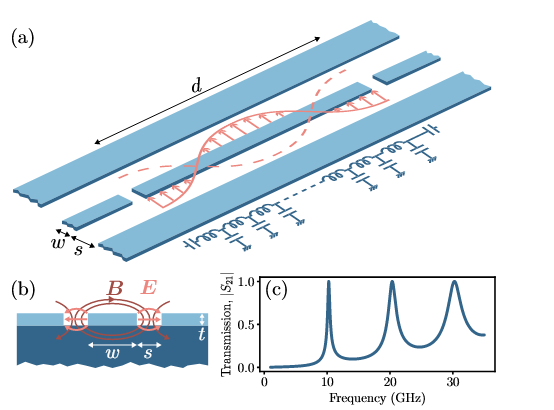
\includegraphics[width=0.8\textwidth]{img/cpw.png}
  \caption{CPW 谐振器示意图（图 2a/2b）}
\end{figure}
\subparagraph{场分布与传播模式：quasi‑TEM } 
\begin{itemize}
  \item - CPW
在平面上充当传输线，传播方式类似同轴线：把电磁场限制在中心导体与地之间的小体积。
  \item - \textbf{quasi‑TEM
模式}：场一部分在衬底介质中，一部分在衬底上方真空/空气中；但\textbf{最强集中在
gap（缝隙）区域}（这是量子比特与谐振器耦合的关键位置------量子比特通常放在此处以最大化耦合）。
  \item - \textbf{关键设计思想}：通过选择 \(w,s,t\)
及介质相关几何，使场尽量集中在中心导体与地之间，从而\textbf{减少向其他方向辐射}，并最大化与量子比特的耦合强度。

\end{itemize}
\paragraph{\texorpdfstring{5.传输线参数：用 \(l_0,c_0\)
把几何``压缩''为可计算模型}{5. 传输线参数：用 l\_0,c\_0 把几何``压缩''为可计算模型}}\label{ux4f20ux8f93ux7ebfux53c2ux6570ux7528-l_0c_0-ux628aux51e0ux4f55ux538bux7f29ux4e3aux53efux8ba1ux7b97ux6a21ux578b}

\subparagraph{5.1
两个单位长度参数}\label{ux4e24ux4e2aux5355ux4f4dux957fux5ea6ux53c2ux6570}

\begin{itemize}
\tightlist
\item
  单位长度电感 \(l_0\)（由几何和穿透深度决定）
\item
  单位长度对地电容 \(c_0\)（由几何和介电常数决定）
\end{itemize}

\subparagraph{5.2
两个最常用派生量（必须会背）}\label{ux4e24ux4e2aux6700ux5e38ux7528ux6d3eux751fux91cfux5fc5ux987bux4f1aux80cc}

\[Z_r=\sqrt{\frac{l_0}{c_0}},\qquad v_0=\frac{1}{\sqrt{l_0c_0}}\] -
典型量级（图中给出）： -
\(Z_r\sim 50~\Omega\)（与标准微波阻抗匹配，便于连接外部设备） -
\(v_0\sim 1.3\times10^8~\text{m/s}\)（约真空光速的
1/3，由有效介电常数决定）

\subparagraph{5.3
几何如何影响阻抗（工程要点）}\label{ux51e0ux4f55ux5982ux4f55ux5f71ux54cdux963bux6297ux5de5ux7a0bux8981ux70b9}

\begin{itemize}
\tightlist
\item
  改变 \(w,s,t\) 会改变 \(l_0,c_0\)，进而改变 \(Z_r\)。
\item
  \textbf{常见技巧}：让 \(w/s\)
  近似保持恒定，可在改变线宽的同时保持近似恒阻抗------便于端口做宽（易于
  bonding 和连接）、腔体内部做窄（减小模体积以增强与量子比特的耦合）。
\end{itemize}


\paragraph{ 6.``谐振腔''从哪里来：边界条件 +
有限长度}\label{ux8c10ux632fux8154ux4eceux54eaux91ccux6765ux8fb9ux754cux6761ux4ef6-ux6709ux9650ux957fux5ea6}

把长度为 \(d\)
的传输线段两端施加边界条件即可形成谐振器------相当于在传输线上形成驻波。

\subparagraph{6.1
两类边界条件}\label{ux4e24ux7c7bux8fb9ux754cux6761ux4ef6}

\begin{itemize}
\tightlist
\item
  \textbf{开路端（open）}：端点电流为零（可用中心导体做 gap 实现，gap
  形成高阻抗）
\item
  \textbf{短路端（short/grounded）}：端点电压为零（直接接地）
\end{itemize}

\subparagraph{\texorpdfstring{6.2 \(\lambda/2\) 与 \(\lambda/4\)
谐振器（频率公式必须熟）}{6.2 \textbackslash{}lambda/2 与 \textbackslash{}lambda/4 谐振器（频率公式必须熟）}}\label{lambda2-ux4e0e-lambda4-ux8c10ux632fux5668ux9891ux7387ux516cux5f0fux5fc5ux987bux719f}

\begin{itemize}
\item
  \textbf{两端开路（open-open）} → \(\lambda/2\) 谐振器：
  \[f_0=\frac{v_0}{2d},\qquad f_m=(m+1)f_0\]
  （电压驻波：两端为波腹，中间为波节）
\item
  \textbf{一端开路一端短路（open-short）} → \(\lambda/4\) 谐振器：
  \[f_0=\frac{v_0}{4d}\] （电压驻波：开路端为波腹，短路端为波节）
\end{itemize}

\subparagraph{6.3
典型频段与极端例子（图中文字给出的信息）}\label{ux5178ux578bux9891ux6bb5ux4e0eux6781ux7aefux4f8bux5b50ux56feux4e2dux6587ux5b57ux7ed9ux51faux7684ux4fe1ux606f}

\begin{itemize}
\tightlist
\item
  \textbf{典型设计}：\(d=1\) cm、\(v_0=1.3\times10^8\) m/s →
  \(f_0\approx 6.5\) GHz（处于 circuit QED 常用频段）。
\item
  \textbf{高频上限}：受超导能隙限制（超过能隙会产生准粒子损耗）；对
  \textbf{Al}，图中给出约 \textbf{82 GHz} 的量级。
\item
  \textbf{低频极端}：可通过超长蛇形线实现低频率，例如 \(d=0.68\)
  m，\(f_0=92\) MHz；但在 \(10\) mK
  下该频率的热占据数可能仍不小（图中给出基模热占据约 \(\sim 1.8\)
  的量级），因此不一定在真空态。
\item
  \textbf{circuit QED 常用频率范围}：\textbf{5--15
  GHz}（此频段兼顾了低温条件、微波电子学成熟度、以及量子比特频率设计的灵活性）。
\end{itemize}


\paragraph{\texorpdfstring{7.
耦合与损耗：\(Q_{\text{int}}, Q_{\text{ext}}, Q_L\)
一套逻辑}{7. 耦合与损耗：Q\_\{\textbackslash{}text\{int\}\}, Q\_\{\textbackslash{}text\{ext\}\}, Q\_L 一套逻辑}}\label{ux8026ux5408ux4e0eux635fux8017q_textint-q_textext-q_l-ux4e00ux5957ux903bux8f91}

\subparagraph{7.1 外耦合怎么做（图 2a \&
文字）}\label{ux5916ux8026ux5408ux600eux4e48ux505aux56fe-2a-ux6587ux5b57}

\begin{itemize}
\tightlist
\item
  输入/输出端口通常通过\textbf{电容耦合}到外部传输线（这样才能把信号送进/取出谐振器，又不至于严重破坏其量子性）。
\item
  耦合电容可由：

  \begin{itemize}
  \tightlist
  \item
    简单 gap 形成的电容
  \item
    或叉指电容（interdigitated capacitors，可精确控制电容值）
  \end{itemize}
\end{itemize}

\subparagraph{7.2
两类损耗的物理起源}\label{ux4e24ux7c7bux635fux8017ux7684ux7269ux7406ux8d77ux6e90}

\begin{itemize}
\tightlist
\item
  \textbf{内损耗（internal）}：与不可控自由度耦合导致能量耗散

  \begin{itemize}
  \tightlist
  \item
    介质与导体表面/界面损耗（主要是非晶态介质中的两能级系统 TLS）
  \item
    衬底介质损耗（如声子激发）
  \item
    非平衡准粒子（超导能隙未被完全打开的激发）
  \item
    磁通涡旋运动（若存在 trapped flux）
  \item
    \textbf{TLS（two-level systems）}
    尤为重要------它们存在于各种无序介质中（如氧化物层、表面吸附物），尤其在电场强的界面区域影响最大
  \end{itemize}
\item
  \textbf{外损耗（external）}：与输入/输出端口耦合导致能量泄露（读出/驱动需要，但会降低
  Q------这是必要的代价）
\end{itemize}

\subparagraph{7.3 总耗散率与加载
Q（必须会用）}\label{ux603bux8017ux6563ux7387ux4e0eux52a0ux8f7d-qux5fc5ux987bux4f1aux7528}

\[\kappa_m=\kappa_{\text{ext},m}+\kappa_{\text{int},m}\]
\[Q_{L,m}=\left(Q_{\text{ext},m}^{-1}+Q_{\text{int},m}^{-1}\right)^{-1}\]
- 工艺进步后，图中文字给出：\textbf{\(Q_{\text{int}}\sim 10^5\)}
已较常见。 -
\textbf{过耦合（overcoupled）}：\(Q_{\text{ext}}<Q_{\text{int}}\)（线宽主要由外耦合决定，利于``快测量''------信号能快速进出谐振器）
-
\textbf{欠耦合（undercoupled）}：\(Q_{\text{ext}}>Q_{\text{int}}\)（线宽主要由内损耗决定；若内损耗也很小，可用于长时间存储微波光子------量子存储器）


\paragraph{8. 为什么 2D CPW
容易实现强耦合：零点涨落更大}\label{ux4e3aux4ec0ux4e48-2d-cpw-ux5bb9ux6613ux5b9eux73b0ux5f3aux8026ux5408ux96f6ux70b9ux6da8ux843dux66f4ux5927}

\subparagraph{8.1
电压零点涨落（图中文字的典型数值链）}\label{ux7535ux538bux96f6ux70b9ux6da8ux843dux56feux4e2dux6587ux5b57ux7684ux5178ux578bux6570ux503cux94fe}

给一组典型参数（示例）：\(L\sim0.8\) nH、\(C\sim0.4\)
pF、\(\omega_r/2\pi\sim 8\)
GHz、\(Z_r\sim50\Omega\)，可得基态电压零点涨落量级：
\[\Delta V_0\simeq \sqrt{\frac{\hbar\omega_r}{2C}}\sim 1~\mu\text{V}\]
（推导：谐振器基态能量 \(\hbar\omega_r/2 = C(\Delta V_0)^2/2\)）

\subparagraph{8.2 横向尺寸可做得很小 →
电场零点涨落更大}\label{ux6a2aux5411ux5c3aux5bf8ux53efux505aux5f97ux5f88ux5c0f-ux7535ux573aux96f6ux70b9ux6da8ux843dux66f4ux5927}

\begin{itemize}
\tightlist
\item
  常用横向几何：\(w\sim 10~\mu\text{m}\)，\(s\sim 5~\mu\text{m}\)。
\item
  进一步缩小到亚微米时，会受超导薄膜\textbf{穿透深度}限制（图中给
  \textbf{100--200 nm}
  量级------若线宽小于穿透深度，电感会增加，阻抗变化）。
\item
  用 \(\Delta V_0\sim 1~\mu\text{V}\)、\(s\sim 5~\mu\text{m}\)
  估算电场零点涨落：
  \[\Delta E_0\approx \frac{\Delta V_0}{s}\sim 0.2~\text{V/m}\]
\item
  \textbf{图中文字结论}：这比 3D 腔 QED
  的典型零点电场强\textbf{至少大两个数量级}；配合超导人工原子的大电偶极矩（约瑟夫森结的相位涨落对应大有效电荷），形成
  circuit QED 的强光-物质耦合优势（\(g/2\pi\) 可达几十到几百 MHz，而 3D
  腔 QED 通常只有几十 kHz）。
\end{itemize}


\paragraph{9.
量子化推导主线（从``电报模型''到``模态谐振子''）}\label{ux91cfux5b50ux5316ux63a8ux5bfcux4e3bux7ebfux4eceux7535ux62a5ux6a21ux578bux5230ux6a21ux6001ux8c10ux632fux5b50}

这一部分的逻辑是：\textbf{离散电路 → 连续场 → 波动方程 → 正常模 →
每模一个谐振子 →
升格为量子算符}。这是从经典传输线到量子谐振子的标准路径。

\subparagraph{9.1
为什么要走这条路？}\label{ux4e3aux4ec0ux4e48ux8981ux8d70ux8fd9ux6761ux8def}

虽然集总 LC
谐振子可以直接量子化，但传输线谐振器是分布参数系统，有多个模式。必须通过正常模分解，才能正确写出每个模式的量子化形式。

\subparagraph{9.2 离散电报模型（图 3）与哈密顿量（式
6）}\label{ux79bbux6563ux7535ux62a5ux6a20ux578bux56fe-3ux4e0eux54c8ux5bc6ux987fux91cfux5f0f-6}

把传输线离散成 \(N\) 段（每段 \(\delta x\)）： - 串联电感
\(L_0=\delta x\,l_0\)（每段储存磁能） - 并联对地电容
\(C_0=\delta x\,c_0\)（每段储存电能） - 节点变量：磁通
\(\Phi_n\)（类比``位置''）、电荷 \(Q_n\)（类比``动量''）

经典哈密顿量（每个节点的电能 + 相邻节点间的磁能）：
\[H=\sum_{n=0}^{N-1}\left[\frac{Q_n^2}{2C_0}+\frac{(\Phi_{n+1}-\Phi_n)^2}{2L_0}\right]\]

\subparagraph{9.3 连续极限（式
7）与变量定义}\label{ux8fdeux7eedux6781ux9650ux5f0f-7ux4e0eux53d8ux91cfux5b9aux4e49}

取 \(\delta x\to 0\)，定义连续场：
\[\Phi(x_n)=\Phi_n,\qquad Q(x_n)=\frac{Q_n}{\delta x}\]
得到连续哈密顿量：
\[H=\int_0^d dx\left[\frac{Q(x,t)^2}{2c_0}+\frac{(\partial_x\Phi(x,t))^2}{2l_0}\right]\]
并有共轭关系： \[Q(x,t)=c_0\,\partial_t\Phi(x,t)\]
广义磁通与电压的关系： \[\Phi(x,t)=\int_{-\infty}^{t}dt'\,V(x,t')\]
（磁通是电压的时间积分，类比于力学中的位移是速度的时间积分）

\subparagraph{9.4 波动方程（式
8）}\label{ux6ce2ux52a8ux65b9ux7a0bux5f0f-8}

由哈密顿方程可得：
\[v_0^2\partial_x^2\Phi-\partial_t^2\Phi=0,\qquad v_0=\frac{1}{\sqrt{l_0c_0}}\]
这是一维波动方程，\(v_0\) 是波速。

\subparagraph{9.5 正常模展开（式
9--10）}\label{ux6b63ux5e38ux6a20ux5c55ux5f00ux5f0f-910}

解可写为正常模叠加（时间部分简谐振动 × 空间分布）：
\[\Phi(x,t)=\sum_{m=0}^{\infty}u_m(x)\Phi_m(t)\] 其中时间部分满足
\(\ddot{\Phi}_m=-\omega_m^2\Phi_m\)，空间模函数为：
\[u_m(x)=A_m\cos(k_m x+\varphi_m),\quad k_m=\omega_m/v_0\]
（这是波动方程的通解形式，具体由边界条件决定 \(k_m\) 和 \(\varphi_m\)）

\subparagraph{9.6 开路端边界条件（式 11）与归一化（式
12）}\label{ux5f00ux8defux7aefux8fb9ux754cux6761ux4ef6ux5f0f-11ux4e0eux5f52ux4e00ux5316ux5f0f-12}

开路端电流为零：
\[I(x)= -\frac{1}{l_0}\partial_x\Phi(x,t),\quad I(0)=I(d)=0\] 这要求
\(\partial_x\Phi(0)=\partial_x\Phi(d)=0\)，即 \(u_m'(0)=u_m'(d)=0\)。

模函数正交归一化条件（能量正交）：
\[\int_0^d dx\,u_m(x)u_{m'}(x)=\delta_{mm'}\] 图中文字给出一种结果：可取
\(A_m=\sqrt{2}\)（并指出这意味着模幅随长度按 \(\sqrt{d}\)
标度变化------腔越长，单位长度的场强越小）。

\subparagraph{9.7 模态哈密顿量（式 13）→
一组独立谐振子}\label{ux6a21ux6001ux54c8ux5bc6ux987fux91cfux5f0f-13-ux4e00ux7ec4ux72ecux7acbux8c10ux632fux5b50}

将展开代入原哈密顿量，利用正交性可得：
\[H=\sum_{m=0}^{\infty}\left[\frac{Q_m^2}{2C_r}+\frac{1}{2}C_r\omega_m^2\Phi_m^2\right]\]
其中： - \(C_r=c_0d\)（谐振器总电容） - \(Q_m=C_r\dot{\Phi}_m\)（第
\(m\) 模的广义电荷） -
\textbf{物理意义}：每个模式都是一个独立的谐振子，有自己有效的``质量''(\(C_r\))和``弹簧常数''(\(C_r\omega_m^2\))

\subparagraph{9.8 量子化（式
14--16）}\label{ux91cfux5b50ux5316ux5f0f-1416}

将 \(\Phi_m,Q_m\) 升格为算符，满足
\([\hat{\Phi}_m,\hat{Q}_{m'}]=i\hbar\delta_{mm'}\)，引入产生湮灭算符：
\[\hat{\Phi}_m=\sqrt{\frac{\hbar Z_m}{2}}(\hat a_m^\dagger+\hat a_m)\]
\[\hat{Q}_m=i\sqrt{\frac{\hbar}{2Z_m}}(\hat a_m^\dagger-\hat a_m)\]
其中模阻抗 \(Z_m=\sqrt{L_m/C_r}\)，\(L_m^{-1}=C_r\omega_m^2\)。

最终量子化哈密顿量（忽略零点能的紧凑形式）：
\[\hat H=\sum_{m=0}^{\infty}\hbar\omega_m\,\hat a_m^\dagger\hat a_m\]

\subparagraph{9.9
文中强调的``简化与扩展''}\label{ux6587ux4e2dux5f3aux8c03ux7684ux7b80ux5316ux4e0eux6269ux5c55}

\begin{itemize}
\tightlist
\item
  \textbf{简化假设}：常为简化忽略端口耦合电容对边界条件/模函数/频率的影响；但实际中耦合电容会：

  \begin{itemize}
  \tightlist
  \item
    改变边界条件（从理想开路变为电容负载）
  \item
    改变模函数形状和频率（产生频率偏移）
  \item
    引入外部耗散（决定 \(Q_{\text{ext}}\)）
  \end{itemize}
\item
  \textbf{非线性扩展}：在中心导体中嵌入约瑟夫森结可引入 \textbf{Kerr
  非线性}（\(\propto (\hat a^\dagger\hat a)^2\) 项），用于：

  \begin{itemize}
  \tightlist
  \item
    近量子极限参量放大
  \item
    分岔放大（bifurcation amplification）
  \item
    研究量子加热（quantum heating）
  \item
    产生非经典态（压缩态、猫态）
  \end{itemize}
\item
  更一般的含非均匀/嵌入结的处理有专门文献（如 Bourassa
  等），涉及如何将结作为集总非线性元件耦合到多模场中。
\end{itemize}


\paragraph{逻辑链总结}\label{ux903bux8f91ux94feux603bux7ed3}

\textbf{为什么需要} → 谐振器是 circuit QED
的核心元件（量子存储器/读出接口）

\textbf{怎么构成} → CPW 结构（中心导体 + 间隙 +
地），通过边界条件形成驻波

\textbf{用什么描述} → 单位长度参数 \(l_0,c_0\) → 特性阻抗 \(Z_r\)、波速
\(v_0\) → 频率 \(f_m\)

\textbf{如何工作} → 边界条件决定模式频率 → 品质因数 \(Q\)
描述能量保持能力 → \(Q_{\text{int}}\)（材料/工艺限制） vs
\(Q_{\text{ext}}\)（耦合设计）

\textbf{为什么强耦合} → 小横向尺寸 → 大零点电场涨落 → 强耦合强度 \(g\)

\textbf{如何量子化} → 离散电报方程 → 连续场 → 波动方程 → 正常模分解 →
每模独立谐振子 → 升格为量子算符 → 得到光子数态

\subsubsection{3D 腔 (3D Cavities)}\label{b.-3d-ux8154-3d-cavities}

\begin{itemize}
\item
  ~ \textbf{结构}: 挖空的金属块（如矩形腔、同轴腔）。
\item
  ~ \textbf{优势}: 极高的 Q 值 (\(10^6 - 10^8\))。
\item
  ~ \textbf{原因}: 电磁场主要分布在真空中，表面参与率极低，受表面 TLS
  影响小。
\item
  ~ \textbf{应用}: 作为长寿命的量子存储器。
\end{itemize}

\textbf{3. 引入非线性：约瑟夫森结 (Josephson
Junction)}
\begin{itemize}
\tightlist
\item
  ~ \textbf{为什么需要非线性？}
\end{itemize}

~ ~ * ~ LC 振荡器是\textbf{线性}的，能级间隔是等距的
(\(\hbar \omega, 2\hbar \omega, \dots\))。

~ ~ * ~ 如果你想从 \(|0\rangle\) 激发到
\(|1\rangle\)，同样的脉冲会把你激发到
\(|2\rangle, |3\rangle \dots\)。你无法单独控制 \(|0\rangle\) 和
\(|1\rangle\) 作为一个\textbf{量子比特}。

~ ~ * ~ 我们需要\textbf{非谐性}，使得 \(\omega_{01} \neq \omega_{12}\)。

\begin{itemize}
\tightlist
\item
  ~ \textbf{约瑟夫森结}:
\end{itemize}

~ ~ * ~ \textbf{结构}: 超导体-绝缘体-超导体。

~ ~ * ~ \textbf{物理}: 非耗散的非线性电感。

~ ~ * ~ \textbf{方程}: \(I = I_c \sin \varphi\)
(电流与相位的正弦关系，而非线性的 \(I \propto \Phi\))。

~ ~ * ~ \textbf{势能}: \(U(\varphi) = -E_J \cos \varphi\)
(余弦势阱，而非 LC 的抛物线势阱)。

~ ~ * ~ 正是这个余弦势阱提供了能级的不等间距，使得我们可以制造出
Transmon 等量子比特。

\subsubsection{The transmon artificial
atom}\label{c.-the-transmon-artificial-atom}


\paragraph{1. 动机：为什么需要
Transmon（非线性人工原子）？}\label{ux52a8ux673aux4e3aux4ec0ux4e48ux9700ux8981-transmonux975eux7ebfux6027ux4ebaux5de5ux539fux5b50}

\subparagraph{1.1
线性谐振子不利于编码量子信息}\label{ux7ebfux6027ux8c10ux632fux5b50ux4e0dux5229ux4e8eux7f16ux7801ux91cfux5b50ux4fe1ux606f}

即使上一节讨论的 LC 谐振器或 CPW
谐振器能被制备到量子基态，要在这类\textbf{线性系统}里实现量子信息处理仍然困难。线性谐振子的能级是等间距的：
\[E_n = \hbar\omega\left(n+\frac{1}{2}\right)\] 这意味着驱动
\(|0\rangle \rightarrow |1\rangle\) 的脉冲同样会驱动
\(|1\rangle \rightarrow |2\rangle\)、\(|2\rangle \rightarrow |3\rangle\)\ldots{}\ldots{}无法单独控制特定的两个能级作为一个量子比特。

\subparagraph{1.2
量子信息需要非线性}\label{ux91cfux5b50ux4fe1ux606fux9700ux8981ux975eux7ebfux6027}

为了在电路中编码与操控量子信息，需要\textbf{非谐性（anharmonicity）}------即能级间隔不等，使得
\(\omega_{01} \neq \omega_{12} \neq \omega_{23} \dots\)。这样我们可以用频率选择性地驱动特定跃迁，把系统近似看作一个二能级系统（量子比特）。

\subparagraph{1.3
超导的优势：引入非线性但保持低损耗}\label{ux8d85ux5bfcux7684ux4f18ux52bfux5f15ux5165ux975eux7ebfux6027ux4f46ux4fddux6301ux4f4eux635fux8017}

超导材料本身是无损耗的（直流电阻为零），但线性电感（几何电感）只能产生等间距能级。要引入非线性同时保持低损耗，关键元件是\textbf{约瑟夫森结（Josephson
junction, JJ）}。它是唯一能与高 Q
超导谐振器、毫开尔文温度兼容的非线性无源元件。

\subparagraph{1.4 历史点}\label{ux5386ux53f2ux70b9}

约瑟夫森结的物理最早由 Brian Josephson 于 1962
年理论预言，随后在实验中被证实，他也因此获得诺贝尔奖。如今，约瑟夫森结是几乎所有超导量子比特的核心元件。


\paragraph{2. Josephson
结的两条基本关系}\label{josephson-ux7ed3ux7684ux4e24ux6761ux57faux672cux5173ux7cfb}

\subparagraph{2.1 无耗散超电流关系（DC Josephson
效应）}\label{ux65e0ux8017ux6563ux8d85ux7535ux6d41ux5173ux7cfbdc-josephson-ux6548ux5e94}

两个超导电极之间隔着薄绝缘层（\textasciitilde{}1-2
nm）时，库珀对可以通过量子隧穿效应穿过绝缘层，形成无耗散的超电流：
\[I = I_c \sin\varphi\] 其中： - \(\varphi = \varphi_2 - \varphi_1\)
是两个超导电极的宏观波函数相位差 - \(I_c\)
是\textbf{临界电流}------结在库珀对被破坏前可承受的最大超电流，由结的尺寸、材料和温度决定

\textbf{物理意义}：即使结两端电压为零，也可以有持续的超电流流动（直流约瑟夫森效应）。电流与相位差的正弦关系是\textbf{非线性的根源}。

\subparagraph{2.2 相位与电压关系（AC Josephson
效应）}\label{ux76f8ux4f4dux4e0eux7535ux538bux5173ux7cfbac-josephson-ux6548ux5e94}

当结两端有电压 \(V\) 时，相位差随时间演化：
\[\frac{d\varphi}{dt} = \frac{2\pi}{\Phi_0}V\]
其中磁通量子（超导通用常数）：
\[\Phi_0 = \frac{h}{2e} \approx 2.07 \times 10^{-15} \text{ Wb}\]

\textbf{物理意义}：恒定电压会产生线性增长的相位，导致交流电流（交流约瑟夫森效应）。这类似于电感两端电压与电流的关系，但约瑟夫森结是非线性的。

常把相位与``广义磁通''\(\Phi(t)\) 联系起来：
\[\varphi(t) = \frac{2\pi}{\Phi_0}\Phi(t) \quad (\text{mod } 2\pi),\qquad \Phi(t) = \int^t dt'\,V(t')\]
但需要注意：\(\varphi\)
是\textbf{紧致变量}（\(\varphi \equiv \varphi + 2\pi\)，因为波函数的相位周期性），而
\(\Phi\) 可取任意实数。


\paragraph{3. Josephson 电感：把 JJ
看作``非线性电感''}\label{josephson-ux7535ux611fux628a-jj-ux770bux4f5cux975eux7ebfux6027ux7535ux611f}

在小信号极限下（\(I \ll I_c\)），约瑟夫森结可以看作一个非线性电感。定义\textbf{约瑟夫森电感}（式
18）：
\[L_J(\Phi) \equiv \left(\frac{\partial I}{\partial \Phi}\right)^{-1} = \frac{\Phi_0}{2\pi I_c \cos(2\pi\Phi/\Phi_0)} = \frac{L_{J0}}{\cos\varphi}\]
其中 \(L_{J0} = \Phi_0/(2\pi I_c)\) 是零偏置时的电感。

\textbf{与几何电感的关键区别}： - 几何电感 \(L\) 是常数，与电流/磁通无关
- 约瑟夫森电感 \(L_J\) \textbf{随工作点（相位/磁通/电流）变化}------当
\(\varphi \rightarrow \pi/2\)
时，\(L_J \rightarrow \infty\)（电流饱和）；当 \(\varphi > \pi/2\)
时，\(L_J\) 变为负值（对应``失稳''区域）

因此，约瑟夫森结在低于临界电流时可视为\textbf{非线性电感元件}------这正是产生非谐性的物理根源。


\paragraph{4. 能量视角：JJ
产生余弦势阱}\label{ux80fdux91cfux89c6ux89d2jj-ux4ea7ux751fux4f59ux5f26ux52bfux9631}

\subparagraph{4.1 线性电感能量 vs
约瑟夫森能量}\label{ux7ebfux6027ux7535ux611fux80fdux91cf-vs-ux7ea6ux745fux592bux68eeux80fdux91cf}

\begin{itemize}
\tightlist
\item
  \textbf{线性电感}的储能公式：\(E = \int I\,d\Phi = \frac{\Phi^2}{2L}\)，对应\textbf{抛物线势阱}。
\item
  \textbf{约瑟夫森结}的储能（式 19）：
  \[E = -\int I\,d\Phi = -\int I_c\sin\varphi \cdot \frac{\Phi_0}{2\pi}d\varphi = -E_J\cos\varphi + \text{常数}\]
  其中\textbf{约瑟夫森能量}定义为： \[E_J = \frac{\Phi_0 I_c}{2\pi}\]
\end{itemize}

\textbf{结论}：约瑟夫森结对应的是\textbf{余弦势阱}，与 LC
谐振子的二次势完全不同。图 5(a)
对比了余弦势与二次势的形状差异------余弦势在底部稍平坦，但两侧更陡，导致能级不等间距。

\subparagraph{4.2
``人工原子''的由来}\label{ux4ebaux5de5ux539fux5b50ux7684ux7531ux6765}

将 LC 谐振子的几何电感 \(L\) 替换为约瑟夫森结（图 5(b)/(c)
的思路）后，电路变为\textbf{非线性}，能级不再等间隔。如果非谐性和品质因数足够好，能谱类似原子------能级可分辨且非均匀分布，因此称为\textbf{人工原子}。

实际用作量子比特时，通常只取最低两个能级（基态 \(|g\rangle\)
与第一激发态
\(|e\rangle\)）编码量子信息，更高能级（\(|f\rangle, |h\rangle, \dots\)）可能会在门操作中引入泄漏错误，需要额外处理。


\paragraph{5. Transmon
的电路与哈密顿量（核心公式链）}\label{transmon-ux7684ux7535ux8defux4e0eux54c8ux5bc6ux987fux91cfux6838ux5fc3ux516cux5f0fux94fe}

\subparagraph{5.1
电路结构：电容分流的约瑟夫森结}\label{ux7535ux8defux7ed3ux6784ux7535ux5bb9ux5206ux6d41ux7684ux7ea6ux745fux592bux68eeux7ed3}

固定频率 transmon（图 5b）的核心结构： - 一个约瑟夫森结（参数
\(E_J\)、结电容 \(C_J\)） - 并联一个较大的分流电容 \(C_S\)

总电容： \[C_\Sigma = C_J + C_S\]

\textbf{设计思想}：通过增加 \(C_S\) 增大总电容，从而降低充电能
\(E_C\)，使系统进入 \(E_J/E_C \gg 1\) 的 transmon 区。

\subparagraph{5.2 变量定义}\label{ux53d8ux91cfux5b9aux4e49}

\begin{itemize}
\item
  \textbf{电荷数算符}（单位：库珀对数）：
  \[\hat n \equiv \frac{\hat Q}{2e}\] （\(\hat Q\) 是结上的总电荷算符）
\item
  \textbf{相位算符}：
  \[\hat\varphi \equiv \frac{2\pi}{\Phi_0}\hat\Phi \quad (\text{mod } 2\pi)\]
  （\(\hat\Phi\) 是广义磁通算符）
\item
  \textbf{充电能}（charging energy）：
  \[E_C \equiv \frac{e^2}{2C_\Sigma}\]
  这是单个电子（不是库珀对）的充电能------注意因子 2 的来源。
\item
  \textbf{偏置电荷}
  \(n_g\)：来自与外界电荷源的电容耦合（杂散电荷或外加栅压）。通常写为
  \(n_g = Q_g/(2e)\)，其中 \(Q_g\) 是栅电容 \(C_g\) 上的感应电荷。
\end{itemize}

\subparagraph{5.3 Transmon 哈密顿量（式
20）}\label{transmon-ux54c8ux5bc6ux987fux91cfux5f0f-20}

\[\hat H_T = \frac{(\hat Q - Q_g)^2}{2C_\Sigma} - E_J\cos\left(\frac{2\pi\hat\Phi}{\Phi_0}\right) = 4E_C(\hat n - n_g)^2 - E_J\cos\hat\varphi\]

\textbf{物理意义}： - 第一项
\(4E_C(\hat n - n_g)^2\)：电容的充电能，类似于动能项 - 第二项
\(-E_J\cos\hat\varphi\)：约瑟夫森结的势能项 -
两者对易关系：\([\hat\varphi, \hat n] = i\)（类似于位置与动量）

\subparagraph{5.4
能谱的一般形式}\label{ux80fdux8c31ux7684ux4e00ux822cux5f62ux5f0f}

无论参数区间如何，总能写成对角形式：
\[\hat H = \sum_j \hbar\omega_j |j\rangle\langle j|\]
常用本征态标记：\(|g\rangle,|e\rangle,|f\rangle,|h\rangle,\dots\)（有时也用
\(|0\rangle,|1\rangle,|2\rangle,\dots\)；需与谐振器 Fock
态区分时会特别说明）。


\paragraph{\texorpdfstring{6. 关键控制参量：比值 \(E_J/E_C\)
决定量子比特类型}{6. 关键控制参量：比值 E\_J/E\_C 决定量子比特类型}}\label{ux5173ux952eux63a7ux5236ux53c2ux91cfux6bd4ux503c-e_je_c-ux51b3ux5b9aux91cfux5b50ux6bd4ux7279ux7c7bux578b}

\(E_J/E_C\) 是区分不同类型超导电荷量子比特的关键参数。

\subparagraph{\texorpdfstring{6.1 小 \(E_J/E_C\)
区（充电能主导，\(E_J/E_C < 1\)）}{6.1 小 E\_J/E\_C 区（充电能主导，E\_J/E\_C \textless{} 1）}}\label{ux5c0f-e_je_c-ux533aux5145ux7535ux80fdux4e3bux5bfce_je_c-1}

\begin{itemize}
\tightlist
\item
  本征态近似是电荷数算符的本征态 \(|n\rangle\)（局域在特定电荷数）。
\item
  此时能级对 \(n_g\)
  \textbf{极度敏感}：环境中不可避免的电荷涨落会引起跃迁频率大幅波动 →
  严重的电荷噪声退相干（dephasing）。
\item
  这是早期 Cooper Pair Box 的工作区间，相干时间很短。
\end{itemize}

\subparagraph{\texorpdfstring{6.2 Transmon 区：大 \(E_J/E_C\)（典型值
20--80）}{6.2 Transmon 区：大 E\_J/E\_C（典型值 20--80）}}\label{transmon-ux533aux5927-e_je_cux5178ux578bux503c-2080}

通过增大 \(E_J/E_C\)（即增大 \(E_J\) 或减小 \(E_C\)）进入 transmon
区，电荷自由度在余弦势阱中变得\textbf{强烈离域}------波函数在相位空间扩展，电荷数不再是好量子数。

\textbf{结果}：最低几个能级的能量对 \(n_g\) 变得几乎不敏感。图 6 展示了
\(E_J/E_C = 2,10,50\) 时能级随 \(n_g\)
的起伏变化------比值越大，曲线越``平坦''。

\textbf{重要补充}：即使能级对静态 \(n_g\)
不敏感，我们仍然可以用外部交流电压源（通过电容耦合）驱动 transmon
的态间跃迁------这相当于在 \(n_g\) 上施加一个交流调制。

\subparagraph{6.3
代价与收益的权衡}\label{ux4ee3ux4ef7ux4e0eux6536ux76caux7684ux6743ux8861}

增大 \(E_J/E_C\) 带来两个相反的效果： - \textbf{收益}：电荷色散（charge
dispersion）随 \(E_J/E_C\) \textbf{指数级降低}（图中给出
\(\sim e^{-\sqrt{8E_J/E_C}}\) 量级），相干时间大幅延长 -
\textbf{代价}：非谐性（anharmonicity）随 \(E_J/E_C\)
增大而\textbf{缓慢降低}，约为 \(\sim (E_J/E_C)^{-1/2}\) 量级

\textbf{权衡结果}：选择 \(E_J/E_C \sim 20-80\)
可在相干时间（指数增益）和非谐性（幂律损失）之间取得最佳平衡。


\paragraph{7. 在 Transmon
区的近似：从余弦势到弱非简谐振子}\label{ux5728-transmon-ux533aux7684ux8fd1ux4f3cux4eceux4f59ux5f26ux52bfux5230ux5f31ux975eux7b80ux8c10ux632fux5b50}

当 \(E_J/E_C \gg 1\) 时，相位在势阱底部较局域（但不像 Cooper Pair Box
那样局域在电荷数空间），可以把余弦势在最小值附近做泰勒展开。

\subparagraph{\texorpdfstring{7.1 去掉 \(n_g\)
并重写哈密顿量}{7.1 去掉 n\_g 并重写哈密顿量}}\label{ux53bbux6389-n_g-ux5e76ux91cdux5199ux54c8ux5bc6ux987fux91cf}

在 transmon 区，相关低能级的频率对 \(n_g\) 几乎不敏感，因此常将 \(n_g\)
略去，直接写为： \[\hat H_q \approx 4E_C\hat n^2 - E_J\cos\hat\varphi\]

\subparagraph{7.2 余弦展开后的哈密顿量（式
22）}\label{ux4f59ux5f26ux5c55ux5f00ux540eux7684ux54c8ux5bc6ux987fux91cfux5f0f-22}

将 \(\cos\hat\varphi\) 在 \(\hat\varphi=0\) 附近展开到四阶：
\[\cos\hat\varphi \approx 1 - \frac{\hat\varphi^2}{2} + \frac{\hat\varphi^4}{24} + \mathcal{O}(\hat\varphi^6)\]
代入并忽略常数项，得到：
\[\hat H_q \approx 4E_C\hat n^2 + \frac{1}{2}E_J\hat\varphi^2 - \frac{1}{24}E_J\hat\varphi^4\]

\textbf{物理意义}：transmon
是一个\textbf{弱非简谐振子}------主导项是二次型（简谐振子），非线性来自
\(-\varphi^4\) 项（负号表示非谐性为负）。

\begin{quote}
\textbf{重要警告}（文中脚注）：这种截断近似会导致近似哈密顿量在数学上``下无界''（当
\(\hat\varphi\) 很大时，\(-\varphi^4\) 项会使能量趋于
\(-\infty\)），这是截断余弦级数导致的伪影。使用时应在原希尔伯特空间的\textbf{截断子空间}内谨慎应用，不能外推到高激发态。
\end{quote}

\subparagraph{7.3 引入产生湮灭算符（式
23-24）}\label{ux5f15ux5165ux4ea7ux751fux6e6eux706dux7b97ux7b26ux5f0f-23-24}

选取算符 \(\hat b, \hat b^\dagger\) 使二次部分对角化：
\[\hat\varphi = \left(\frac{2E_C}{E_J}\right)^{1/4}(\hat b^\dagger + \hat b)\]
\[\hat n = \frac{i}{2}\left(\frac{E_J}{2E_C}\right)^{1/4}(\hat b^\dagger - \hat b)\]

\textbf{重要结论}：当 \(E_J/E_C\) 增大时： - \(\hat\varphi\) 的零点涨落
\(\propto (E_C/E_J)^{1/4}\) \textbf{减小}（相位更局域） - 共轭变量
\(\hat n\) 的零点涨落 \(\propto (E_J/E_C)^{1/4}\)
\textbf{增大}（电荷涨落更大）

这正是 transmon
对电荷噪声不敏感的原因------电荷涨落大意味着电荷数不确定，因此外部电荷扰动影响小。

\subparagraph{7.4 得到 Kerr 形式的有效哈密顿量（式
25）}\label{ux5f97ux5230-kerr-ux5f62ux5f0fux7684ux6709ux6548ux54c8ux5bc6ux987fux91cfux5f0f-25}

代入并在旋转波近似下保留``数算符守恒''项（即保留
\(\hat b^\dagger\hat b^\dagger\hat b\hat b\) 形式的项，舍弃
\(\hat b^\dagger\hat b^\dagger + \hat b\hat b\) 等非能量守恒项）：
\[\hat H_q \approx \sqrt{8E_CE_J}\,\hat b^\dagger \hat b - \frac{E_C}{12}(\hat b^\dagger+\hat b)^4 \approx \hbar\omega_q\,\hat b^\dagger \hat b - \frac{E_C}{2}\hat b^\dagger\hat b^\dagger\hat b\hat b\]

其中： \[\hbar\omega_q \approx \sqrt{8E_CE_J} - E_C\]

\textbf{旋转波近似有效的条件}：\(\hbar\omega_q \gg E_C\)，这在 transmon
区（\(E_J/E_C \gg 1\)）很容易满足。

\subparagraph{7.5 三个必须记住的物理量（transmon
区）}\label{ux4e09ux4e2aux5fc5ux987bux8bb0ux4f4fux7684ux7269ux7406ux91cftransmon-ux533a}

\begin{enumerate}
\def\labelenumi{\arabic{enumi}.}
\item
  \textbf{约瑟夫森等离子体频率}（plasma frequency）：
  \[\omega_p = \frac{\sqrt{8E_CE_J}}{\hbar}\]
  对应余弦势阱底部``小振动''的角频率------即如果把余弦近似为抛物线得到的简谐振子频率。
\item
  \textbf{基态到第一激发态的跃迁频率}：
  \[\omega_{ge} \approx \omega_p - \frac{E_C}{\hbar}\]
  比等离子体频率略低，偏移量正好是 \(E_C/\hbar\)。
\item
  \textbf{非谐性}（anharmonicity）：
  \[\alpha \equiv \omega_{ef} - \omega_{ge} \approx -\frac{E_C}{\hbar}\]
  典型量级：\(E_C/h \sim 100\text{–}400\) MHz，所以
  \(\alpha/2\pi \sim -100\) 到 \(-400\) MHz。
\end{enumerate}

\subparagraph{7.6
为什么``非线性虽小但仍够用''}\label{ux4e3aux4ec0ux4e48ux975eux7ebfux6027ux867dux5c0fux4f46ux4ecdux591fux7528}

尽管 \(E_C \ll \hbar\omega_q\)（即非谐性远小于跃迁频率），但
\(|\alpha|\) 通常仍在 \(100\) MHz 量级，而量子比特的线宽 \(\gamma\)
通常在 kHz-MHz 量级。因此： \[|\alpha| \gg \gamma\]
能级不等间距仍远大于谱线宽度，从而可以用频率选择性地驱动
\(|g\rangle \leftrightarrow |e\rangle\) 跃迁而不激发到 \(|f\rangle\)。

\textbf{同时要牢记}：transmon
本质上是多能级系统，在一些高保真度门操作或特定实验中，\(|f\rangle\)
态的布居可能会成为限制因素，需要额外考虑。


\paragraph{8. Flux-tunable Transmon：用 SQUID
实现频率可调}\label{flux-tunable-transmonux7528-squid-ux5b9eux73b0ux9891ux7387ux53efux8c03}

\subparagraph{8.1 电路思想}\label{ux7535ux8defux601dux60f3}

用一个 SQUID（两个并联的约瑟夫森结）替代单个约瑟夫森结，使等效 \(E_J\)
受外加磁通 \(\Phi_x\) 控制，从而量子比特频率可调。图 5(c)
展示了这种结构。

\subparagraph{8.2 SQUID 情况的哈密顿量（式
26）}\label{squid-ux60c5ux51b5ux7684ux54c8ux5bc6ux987fux91cfux5f0f-26}

\[\hat H_T = 4E_C\hat n^2 - E_{J1}\cos\hat\varphi_1 - E_{J2}\cos\hat\varphi_2\]

外加磁通 \(\Phi_x\) 穿过 SQUID
环路，且忽略环路几何电感时（即环路电感远小于约瑟夫森电感），有磁通量子化条件：
\[\hat\varphi_1 - \hat\varphi_2 = 2\pi\frac{\Phi_x}{\Phi_0} \quad (\text{mod } 2\pi)\]

\subparagraph{8.3
约化为单结形式}\label{ux7ea6ux5316ux4e3aux5355ux7ed3ux5f62ux5f0f}

定义平均相位
\(\hat\varphi = (\hat\varphi_1 + \hat\varphi_2)/2\)，通过三角恒等式可化为（式
27）：
\[\hat H_T = 4E_C\hat n^2 - E_J(\Phi_x)\cos(\hat\varphi - \varphi_0)\]

\subparagraph{8.4 有效约瑟夫森能量（式
28）}\label{ux6709ux6548ux7ea6ux745fux592bux68eeux80fdux91cfux5f0f-28}

\[E_J(\Phi_x) = E_{J\Sigma} \cos\left(\pi\frac{\Phi_x}{\Phi_0}\right) \sqrt{1 + d^2 \tan^2\left(\pi\frac{\Phi_x}{\Phi_0}\right)}\]
其中： - \(E_{J\Sigma} = E_{J1} + E_{J2}\)（总约瑟夫森能量） -
\(d = \frac{E_{J2} - E_{J1}}{E_{J\Sigma}}\)（结的不对称度）

相位偏置 \(\varphi_0 = \arctan\!\left(d\tan(\pi\Phi_x/\Phi_0)\right)\)
对\textbf{静态磁通}通常可忽略（因仅影响波函数相位，不改变能谱）。

\textbf{对称结特例}（\(E_{J1} = E_{J2} = E_J\)，\(d=0\)）：
\[E_J(\Phi_x) = 2E_J \left|\cos\left(\pi\frac{\Phi_x}{\Phi_0}\right)\right|\]

\subparagraph{8.5
可调频率与调谐速度}\label{ux53efux8c03ux9891ux7387ux4e0eux8c03ux8c10ux901fux5ea6}

量子比特频率随磁通变化：
\[\omega_q(\Phi_x) \approx \frac{\sqrt{8E_C E_J(\Phi_x)} - E_C}{\hbar}\]

\textbf{实验参数}： - 调谐范围：约 \textbf{1-2 GHz}（典型值） -
调谐速度：可快到 \textbf{10-20 ns}（通过快速磁通脉冲） -
动态范围可通过增加磁通线带宽扩展

这种可调谐性用于多种应用： - 快速将量子比特调到与谐振器共振（实现 iSWAP
门） - 调到特定避免交叉点（实现 CZ 门） -
调到远离谐振器（减少耦合，保护相干性）

\subparagraph{8.6
代价：磁通噪声退相干}\label{ux4ee3ux4ef7ux78c1ux901aux566aux58f0ux9000ux76f8ux5e72}

额外的调谐旋钮会引入磁通噪声导致的退相干风险。磁通噪声来源包括： -
外部环境中的随机磁通涨落 - 临近涡旋的运动 - 电流源的噪声

\textbf{不对称性的权衡}： - 更大的结不对称 \(d\) →
调谐范围减小（\(E_J(\Phi_x)\) 的最小值变大） -
但也会使器件在磁通偏置点对磁通噪声\textbf{更不敏感}（因为
\(dE_J/d\Phi_x\) 更小）

这是一个典型的``可调谐性 vs 噪声敏感性''的权衡。

\subparagraph{8.7 拓展方向}\label{ux62d3ux5c55ux65b9ux5411}

文中提到实现``电压可调''的 transmon：例如用\textbf{半导体纳米线}替代
SQUID 环路，通过栅压控制结的传输特性，实现电学可调的约瑟夫森能量。


\paragraph{9. 图像与直观总结（对应图 5 与图
6）}\label{ux56feux50cfux4e0eux76f4ux89c2ux603bux7ed3ux5bf9ux5e94ux56fe-5-ux4e0eux56fe-6}

\subparagraph{图 5
的核心信息}\label{ux56fe-5-ux7684ux6838ux5fc3ux4fe1ux606f}

\begin{itemize}
\tightlist
\item
  \textbf{图 5(a)}：transmon 的余弦势阱（实线）与 LC
  的二次势（虚线）对比。余弦势底部稍平坦，但两侧更陡，导致能级
  \(|g\rangle,|e\rangle,|f\rangle,|h\rangle,\dots\)
  不等间隔，非谐性量级约为 \(-E_C\)。
\item
  \textbf{图 5(b)}：固定频率 transmon
  的电路图------单个约瑟夫森结并联分流电容。
\item
  \textbf{图 5(c)}：频率可调 transmon------用
  SQUID（两个结）替代单结，通过外磁通控制等效 \(E_J\)。
\end{itemize}

\subparagraph{图 6
的核心信息}\label{ux56fe-6-ux7684ux6838ux5fc3ux4fe1ux606f}

展示不同 \(E_J/E_C\) 比值下，最低三个能级对 offset charge \(n_g\)
的敏感性： - \(E_J/E_C = 2\)：能级剧烈振荡，对电荷噪声极度敏感（早期
Cooper Pair Box） - \(E_J/E_C = 10\)：振荡幅度显著减小 -
\(E_J/E_C = 50\)：能级几乎平坦，对 \(n_g\) 不敏感（典型 transmon 区）

\textbf{结论}：比值越大，电荷色散被压制得越彻底------这正是 transmon
获得长相干时间的关键。


\paragraph{10. Transmon
设计参数总结表}\label{transmon-ux8bbeux8ba1ux53c2ux6570ux603bux7ed3ux8868}

\begin{longtable}[]{@{}llll@{}}
\toprule
参数 & 符号 & 典型值 & 作用\tabularnewline
\midrule
\endhead
充电能 & \(E_C/h\) & 100-400 MHz & 决定非谐性
\(\alpha \approx -E_C/\hbar\)\tabularnewline
约瑟夫森能 & \(E_J/h\) & 10-30 GHz & 决定跃迁频率
\(\omega_{ge} \approx \sqrt{8E_CE_J}/\hbar\)\tabularnewline
比值 & \(E_J/E_C\) & 20-80 &
决定电荷噪声敏感性（指数级影响）\tabularnewline
跃迁频率 & \(\omega_{ge}/2\pi\) & 4-8 GHz &
量子比特的工作频率\tabularnewline
非谐性 & \(\alpha/2\pi\) & -100 到 -400 MHz &
确保能级可分辨，\(\alpha \gg \gamma\)\tabularnewline
电荷色散 & \(\epsilon\) & kHz-MHz 量级 & 随 \(E_J/E_C\)
指数减小\tabularnewline
调谐范围（可调版） & \(\Delta\omega/2\pi\) & 1-2 GHz &
通过磁通调节频率的范围\tabularnewline
\bottomrule
\end{longtable}


\subsection{逻辑链总结}\label{ux903bux8f91ux94feux603bux7ed3-1}

\textbf{为什么需要} → 线性谐振子不能做量子比特（能级等距）→ 需要非线性 →
约瑟夫森结提供非线性（余弦势）

\textbf{如何工作} → 电荷能 \(4E_C(\hat n - n_g)^2\) + 约瑟夫森能
\(-E_J\cos\hat\varphi\) → 哈密顿量

\textbf{关键参数} → \(E_J/E_C\)
比值决定量子比特类型：小比值→电荷敏感（相干差），大比值→电荷不敏感（transmon）

\textbf{transmon 区近似} → \(E_J/E_C \gg 1\) → 弱非简谐振子近似 →
\(\hat H \approx \hbar\omega_q \hat b^\dagger \hat b - (E_C/2)\hat b^\dagger\hat b^\dagger\hat b\hat b\)

\textbf{三个关键频率} →
\(\omega_p = \sqrt{8E_CE_J}/\hbar\)（等离子体频率），\(\omega_{ge} \approx \omega_p - E_C/\hbar\)（工作频率），\(\alpha \approx -E_C/\hbar\)（非谐性）

\textbf{可调版本} → SQUID 替代单结 → \(E_J(\Phi_x)\) 受磁通控制 →
频率可调，但引入磁通噪声风险

\textbf{最终结果} → transmon
实现了``长相干时间''（通过电荷噪声指数压制）与``足够非谐性''（\(|\alpha| \gg \gamma\)）的平衡，成为当前超导量子计算的主流量子比特类型

\section{\texorpdfstring{\textbf{LIGHT--MATTER INTERACTION IN
CIRCUIT
QED}}{III. LIGHT--MATTER INTERACTION IN CIRCUIT QED}}\label{iii.-lightmatter-interaction-in-circuit-qed}

（电路 QED 中的光---物质相互作用）


\subsection{A Exchange interaction between a
transmon and an
oscillator}
（transmon 与谐振子之间的交换相互作用）

\subsubsection{\texorpdfstring{\textbf{A1.
场景与耦合方式（从``经典门电压''到``量子谐振子''）}}{A1. 场景与耦合方式（从``经典门电压''到``量子谐振子''）}}\label{a1.-ux573aux666fux4e0eux8026ux5408ux65b9ux5f0fux4eceux7ecfux5178ux95e8ux7535ux538bux5230ux91cfux5b50ux8c10ux632fux5b50}

\begin{itemize}
\tightlist
\item
  前文已引入两大主角：

  \begin{enumerate}
  \def\labelenumi{\arabic{enumi})}
  \tightlist
  \item
    \textbf{量子简谐振子}（微波谐振器的模式）
  \item
    \textbf{transmon 人工原子}
  \end{enumerate}
\item
  transmon 由于需要
  \textbf{较大的电荷能（即较大电容）}，因此很自然地可通过\textbf{电容耦合}接入微波谐振器（见
  Fig.7 的示意）。
\item
  当谐振器在电路中扮演``经典电压源 \(V_g\)''的角色时，可以在 transmon
  哈密顿量中把\textbf{经典门电压}对应的 \textbf{\(n_g\)}
  替换成一个\textbf{量子化的门电荷偏置}： \[
  n_g \ \rightarrow\ -\hat n_r
  \] 其中 \(-\hat n_r\) 表示由谐振器引入、作用在 transmon
  上的量子化电荷偏置（符号正负是文献中的常用约定；文中说明采用该约定，见
  Appendix A）。
\end{itemize}

\subsubsection{\texorpdfstring{\textbf{A2. 多模情况下的总哈密顿量（Eq.
29）}}{A2. 多模情况下的总哈密顿量（Eq. 29）}}\label{a2.-ux591aux6a21ux60c5ux51b5ux4e0bux7684ux603bux54c8ux5bc6ux987fux91cfeq.-29}

耦合后的总系统哈密顿量（Blais et al., 2004）写成： \[
\hat H
=4E_C(\hat n+\hat n_r)^2
- E_J\cos\hat\phi
+\sum_m \hbar\omega_m \hat a_m^\dagger \hat a_m,
\tag{29}
\] 并给出： - \(\hat n\)：transmon 的库珀对数（电荷数）算符\\
- \(\hat\phi\)：结两端超导相位差算符\\
- \(E_C\)：充电能；\(E_J\)：约瑟夫森能\\
- 第 \(m\) 个谐振器模：频率 \(\omega_m\)，产生/湮灭算符
\(\hat a_m^\dagger,\hat a_m\) - 谐振器引入的``门电荷''项： \[
  \hat n_r=\sum_m \hat n_m,\qquad
  \hat n_m=\Big(\frac{C_g}{C_m}\Big)\frac{\hat q_m}{2e},
  \] 其中\\
- \(C_g\)：耦合电容（gate capacitance）\\
- \(C_m\)：第 \(m\) 个模式对应的``模式电容''\\
- \(\hat q_m\)：第 \(m\) 模对 transmon
产生门偏置的电荷坐标（以电荷形式出现）\\
- 文中为简化使用了假设：\\
\[
  C_g \ll C_\Sigma,\ C_m
  \] 其中 \(C_\Sigma\) 是 transmon 的总电容（有效电容）。\\
- 文中说明：对 Eq.(29) 的更完整推导（不仅是简单替换
\(n_g\to -\hat n_r\)，且不依赖上述小电容近似）可见 Appendix A（单个 LC
振子耦合 transmon 的情形）。

\subsubsection{\texorpdfstring{\textbf{A3. 单模近似与等效电路解释（Fig.7
与``black-box
quantization''）}}{A3. 单模近似与等效电路解释（Fig.7 与``black-box quantization''）}}\label{a3.-ux5355ux6a21ux8fd1ux4f3cux4e0eux7b49ux6548ux7535ux8defux89e3ux91cafig.7-ux4e0eblack-box-quantization}

\begin{itemize}
\tightlist
\item
  若 transmon
  频率更接近某一个谐振器模式而远离其他模式，满足近似条件（原文表述）：
  \[
  |\omega_0-\omega_q|\ll|\omega_m-\omega_q|\quad (m\ge 1),
  \] 则可以将 Eq.(29) 中对 \(m\)
  的求和\textbf{截断}为单一项（single-mode approximation）。
\item
  在单模近似下，总系统可视为：\textbf{频率为 \(\omega_r\) 的单一简谐振子
  + transmon}。
\item
  文中特别强调：不论这个``振子模式''在物理上来自

  \begin{itemize}
  \tightlist
  \item
    2D/3D 分布参数谐振器的某一模，或\\
  \item
    集总元件 LC\\
    都可以用\textbf{等效集总元件电路}表示：transmon 电容耦合到
    LC（Fig.7(b)）。
  \end{itemize}
\item
  这种把复杂几何结构``等效成集总元件''的形式化量子化思路，称为
  \textbf{black-box quantization}（Nigg et al., 2012），文中指出会在
  Sec. III.D 更详细讨论。
\item
  文中同时提醒：在很多实验相关情形里，忽略谐振器的\textbf{多模性}会导致不准确预测（将在
  Sec. IV.E 讨论）。
\end{itemize}

\subsubsection{\texorpdfstring{\textbf{A4.
单模下、用产生湮灭算符写出的耦合哈密顿量（Eq.
30）}}{A4. 单模下、用产生湮灭算符写出的耦合哈密顿量（Eq. 30）}}\label{a4.-ux5355ux6a21ux4e0bux7528ux4ea7ux751fux6e6eux706dux7b97ux7b26ux5199ux51faux7684ux8026ux5408ux54c8ux5bc6ux987fux91cfeq.-30}

在单模近似并引入前文的产生/湮灭算符后（谐振器用 \(\hat a\)，transmon
的弱非谐性用 \(\hat b\) 表示），得到： \[
\hat H \approx
\hbar\omega_r \hat a^\dagger\hat a
+\hbar\omega_q \hat b^\dagger\hat b
-\frac{E_C}{2}\hat b^\dagger\hat b^\dagger \hat b\hat b
-\hbar g(\hat b^\dagger-\hat b)(\hat a^\dagger-\hat a).
\tag{30}
\] - \(\omega_r\)：所选谐振器模式频率\\
- \(\omega_q\)：transmon 的（近似）本征频率\\
- \(-\frac{E_C}{2}\hat b^\dagger\hat b^\dagger \hat b\hat b\)：transmon
的 Duffing 型非线性（弱非谐性） - 最后项是``电偶极---电场''型的耦合（以
\((\hat b^\dagger-\hat b)(\hat a^\dagger-\hat a)\) 形式出现）

\textbf{脚注 3（原文要点）}\\
- 可能担心 Eq.(29) 展开后出现 \(\hat n_r^2\)
项；文中说明该项可并入谐振器模式的``充电能''从而导致谐振器频率的重整化，因此为简洁起见省略；更多细节见文中引用的附录公式（A9）、（A10）。

\subsubsection{\texorpdfstring{\textbf{A5. 旋波近似（RWA）与交换型耦合（Eq.
32）}}{A5. 旋波近似（RWA）与交换型耦合（Eq. 32）}}\label{a5.-ux65cbux6ce2ux8fd1ux4f3crwaux4e0eux4ea4ux6362ux578bux8026ux5408eq.-32}

在实验常见的弱耦合条件下： \[
|g|\ll \omega_r,\ \omega_q,
\] 采用 rotating-wave approximation（旋波近似）后，Eq.(30) 化为： \[
\hat H \approx
\hbar\omega_r \hat a^\dagger\hat a
+\hbar\omega_q \hat b^\dagger\hat b
-\frac{E_C}{2}\hat b^\dagger\hat b^\dagger \hat b\hat b
+\hbar g(\hat b^\dagger \hat a+\hat b \hat a^\dagger).
\tag{32}
\] - 最后一项 \(\hbar g(\hat b^\dagger \hat a+\hat b \hat a^\dagger)\)
明确对应``交换（exchange）相互作用''：在两系统间相干交换一个量子。

\subsubsection{\texorpdfstring{\textbf{A6. 耦合强度 \(g\) 的表达式（Eq.
31）及参数含义}}{A6. 耦合强度 g 的表达式（Eq. 31）及参数含义}}\label{a6.-ux8026ux5408ux5f3aux5ea6-g-ux7684ux8868ux8fbeux5f0feq.-31ux53caux53c2ux6570ux542bux4e49}

文中给出振子---transmon（光---物质）耦合强度： \[
g=\omega_r\frac{C_g}{C_\Sigma}\Big(\frac{E_J}{2E_C}\Big)^{1/4}\sqrt{\frac{\pi Z_r}{R_K}}.
\tag{31}
\] 各量定义： - \(Z_r\)：谐振器模式的特征阻抗（characteristic
impedance） -
\(R_K=h/e^2 \approx 25.8~\text{k}\Omega\)：电阻量子（resistance
quantum） - \(\frac{C_g}{C_\Sigma}\)：耦合``分压/分电荷''比例因子 -
\(\Big(\frac{E_J}{2E_C}\Big)^{1/4}\)：与 transmon
的电荷涨落尺度相关（文中指出可由 Eq.(24) 看出这一点）

\subsubsection{\texorpdfstring{\textbf{A7. 用``偶极矩 ×
零点电场''的物理图像理解
\(g\)}}{A7. 用``偶极矩 × 零点电场''的物理图像理解 g}}\label{a7.-ux7528ux5076ux6781ux77e9-ux96f6ux70b9ux7535ux573aux7684ux7269ux7406ux56feux50cfux7406ux89e3-g}

\begin{itemize}
\tightlist
\item
  文中引入一个长度尺度 \(l\)：表示库珀对穿越 transmon
  结隧穿时的等效距离。由此可把 Eq.(31) 诱导性地解释为： \[
  \hbar g = d_0 E_0,
  \] 其中

  \begin{itemize}
  \tightlist
  \item
    \(d_0=2el\,(E_J/32E_C)^{1/4}\)：transmon 的电偶极矩\\
  \item
    \(E_0=(\omega_r/l)(C_g/C_\Sigma)\sqrt{\hbar Z_r/2}\)：谐振器的零点电场（以
    transmon ``看到''的方式定义）
  \end{itemize}
\item
  结论：因为 \(d_0\) 与 \(E_0\) 都可以做得很大（尤其在 transmon 区域
  \(E_J/E_C\) 大时），所以电路 QED
  中的电偶极耦合强度可远大于天然原子在腔 QED 中的耦合。
\end{itemize}

\subsubsection{\texorpdfstring{\textbf{A8.
进一步写成与精细结构常数相关的形式（Eq.
33）与工程提升路径}}{A8. 进一步写成与精细结构常数相关的形式（Eq. 33）与工程提升路径}}\label{a8.-ux8fdbux4e00ux6b65ux5199ux6210ux4e0eux7cbeux7ec6ux7ed3ux6784ux5e38ux6570ux76f8ux5173ux7684ux5f62ux5f0feq.-33ux4e0eux5de5ux7a0bux63d0ux5347ux8defux5f84}

文中进一步把 Eq.(31) 改写成与精细结构常数有关的形式（Devoret et al.,
2007）： \[
g=\omega_r\frac{C_g}{C_\Sigma}\Big(\frac{E_J}{2E_C}\Big)^{1/4}
\sqrt{\frac{Z_r}{Z_{\rm vac}}}\,\sqrt{2\pi\alpha},
\tag{33}
\] 其中 - \(\alpha=Z_{\rm vac}/(2R_K)\)：精细结构常数 -
\(Z_{\rm vac}=\sqrt{\mu_0/\varepsilon_0}\approx 377~\Omega\)：真空阻抗 -
文中指出：这里``相互作用强度''被 \(\frac{Z_r}{Z_{\rm vac}}\) 与
\(\frac{C_g}{C_\Sigma}\) 这类小于 1 的因子削弱；但仍可通过增大
\(E_J/E_C\)（transmon 区域）实现很大的耦合。 - 代价：更大的 \(g\)
往往以减小 transmon
的相对非谐性为代价；文中给出相对非谐性标度（原文表达）： \[
  -\frac{E_C}{\hbar\omega_q}\sim \sqrt{\frac{E_C}{8E_J}}.
  \] - 工程上提升 \(g\) 的方式之一：\textbf{提高谐振器阻抗
\(Z_r\)}，例如用结阵列替代谐振器中心导体（Andersen and Blais, 2017;
Stockklauser et al., 2017）。 - 从 2D 到 3D：3D
谐振腔使模式体积显著变大，从而降低真空电场涨落；但可通过把 transmon
做大（增加偶极矩）在不改变 \(g\) 数量级的情况下补偿（Paik et al.,
2011）。文中形象描述：transmon 在 3D
腔中相当于``天线''，放置在合适位置可强耦合到某一腔模（Fig.7(c)）。

\subsubsection{\texorpdfstring{\textbf{A9. 两能级近似得到 Jaynes--Cummings
哈密顿量（Eq.
34）}}{A9. 两能级近似得到 Jaynes--Cummings 哈密顿量（Eq. 34）}}\label{a9.-ux4e24ux80fdux7ea7ux8fd1ux4f3cux5f97ux5230-jaynescummings-ux54c8ux5bc6ux987fux91cfeq.-34}

为了进一步强化与腔 QED 的类比，文中将 transmon 限制到前两能级
\(\{|g\rangle,|e\rangle\}\)，做替换： \[
\hat b^\dagger\rightarrow \hat\sigma_+ = |e\rangle\langle g|,\qquad
\hat b\rightarrow \hat\sigma_- = |g\rangle\langle e|.
\] 于是从 Eq.(30) 得到著名的 Jaynes--Cummings（JC）模型（Blais et al.,
2004; Haroche and Raimond, 2006）： \[
\hat H_{\rm JC}
=\hbar\omega_r\hat a^\dagger\hat a
+\frac{\hbar\omega_q}{2}\hat\sigma_z
+\hbar g(\hat a^\dagger\hat\sigma_-+\hat a\hat\sigma_+),
\tag{34}
\] 其中采用 \[
\hat\sigma_z=|e\rangle\langle e|-|g\rangle\langle g|.
\] - 最后一项描述``单量子''的相干交换：一个谐振器光子 ↔ transmon
的一个激发。


\subsection{\texorpdfstring{\textbf{B. The Jaynes--Cummings
spectrum}}{B. The Jaynes--Cummings spectrum}}\label{b.-the-jaynescummings-spectrum}

（Jaynes--Cummings 能谱）

\subsubsection{\texorpdfstring{\textbf{B1.
模型地位与适用性（文中评价）}}{B1. 模型地位与适用性（文中评价）}}\label{b1.-ux6a21ux578bux5730ux4f4dux4e0eux9002ux7528ux6027ux6587ux4e2dux8bc4ux4ef7}

\begin{itemize}
\tightlist
\item
  JC
  哈密顿量是\textbf{可精确求解}的模型，能准确描述许多情形：把（天然或人工）原子当作两能级系统，与电磁场的单一模式相互作用。
\item
  在只关心 transmon 前两能级 \(|\sigma\rangle=\{|g\rangle,|e\rangle\}\)
  的实验里，JC 模型常能给出\textbf{定性一致}的结果。
\item
  但文中也强调：要达到\textbf{定量一致}，通常必须考虑

  \begin{enumerate}
  \def\labelenumi{\arabic{enumi})}
  \tightlist
  \item
    transmon 的更高能级\\
  \item
    场的多模性\\
    这点在电路 QED 中经常很关键。尽管如此，JC
    模型仍提供大量重要物理直觉，因此接下来聚焦其谱结构。
  \end{enumerate}
\end{itemize}

\subsubsection{\texorpdfstring{\textbf{B2. 裸态（bare
states）与``总激发数''守恒结构}}{B2. 裸态（bare states）与``总激发数''守恒结构}}\label{b2.-ux88f8ux6001bare-statesux4e0eux603bux6fc0ux53d1ux6570ux5b88ux6052ux7ed3ux6784}

\begin{itemize}
\tightlist
\item
  当 \(g=0\)（无耦合）时，qubit--field 系统的裸态标记为
  \(|\sigma,n\rangle\)，其中

  \begin{itemize}
  \tightlist
  \item
    \(\sigma\in\{g,e\}\) 表示两能级系统状态\\
  \item
    \(n\) 表示谐振器的光子数
  \end{itemize}
\item
  JC 模型具有按``总激发数''分块对角的结构（下文引入算符 \(\hat N_T\)）。
\end{itemize}

\subsubsection{\texorpdfstring{\textbf{B3. 用 Bogoliubov-like
幺正变换对角化（Eq.
35--37）}}{B3. 用 Bogoliubov-like 幺正变换对角化（Eq. 35--37）}}\label{b3.-ux7528-bogoliubov-like-ux5e7aux6b63ux53d8ux6362ux5bf9ux89d2ux5316eq.-3537}

文中给出 dressed 态可由幺正变换从裸态获得： \[
|\overline{\sigma,n}\rangle=\hat U^\dagger|\sigma,n\rangle,
\] 其中变换取（Boissonneault et al., 2009; Carbonaro et al., 1979）： \[
\hat U=\exp\!\Big[\Lambda(\hat N_T)\big(\hat a^\dagger\hat\sigma_- - \hat a\hat\sigma_+\big)\Big],
\tag{35}
\] 并定义 \[
\Lambda(\hat N_T)=\frac{\arctan\!\big(2\lambda\sqrt{\hat N_T}\big)}{2\sqrt{\hat N_T}}.
\tag{36}
\] 这里 - \[
  \hat N_T=\hat a^\dagger\hat a+\hat\sigma_+\hat\sigma_-
  \] 是\textbf{总激发数算符}；文中指出它与 \(\hat H_{\rm JC}\) 对易。 -
\[
  \lambda=\frac{g}{\Delta},\qquad \Delta=\omega_q-\omega_r
  \] 其中 \(\Delta\) 是 qubit--resonator 失谐（detuning）。

对角化后： \[
\hat H_D=\hat U^\dagger \hat H_{\rm JC}\hat U
=\hbar\omega_r\hat a^\dagger\hat a
+\frac{\hbar\omega_q}{2}\hat\sigma_z
-\frac{\hbar\Delta}{2}\Big(1-\sqrt{1+4\lambda^2\hat N_T}\Big)\hat\sigma_z.
\tag{37}
\]

\subsubsection{\texorpdfstring{\textbf{B4. JC
能谱的``双态（doublets）''结构与本征能量（Eq.
38）}}{B4. JC 能谱的``双态（doublets）''结构与本征能量（Eq. 38）}}\label{b4.-jc-ux80fdux8c31ux7684ux53ccux6001doubletsux7ed3ux6784ux4e0eux672cux5f81ux80fdux91cfeq.-38}

由 Eq.(37) 可直接读出 dressed 态能量；JC
谱由固定激发数的双重态（doublet） \(\{|g,n\rangle,\ |e,n-1\rangle\}\)
构成（文中脚注 4 说明：推导中给 \(\hat H_D\) 加了 \(\hbar\omega_r/2\)
的整体能量平移，这不影响物理结论）。

能量为： \[
E_{g,n}=n\hbar\omega_r-\frac{\hbar}{2}\sqrt{\Delta^2+4g^2n},
\qquad
E_{e,n-1}=n\hbar\omega_r+\frac{\hbar}{2}\sqrt{\Delta^2+4g^2n}.
\tag{38}
\] 并给出基态 \(|g,0\rangle\) 的能量： \[
E_{g,0}=-\frac{\hbar\omega_q}{2}.
\]

\subsubsection{\texorpdfstring{\textbf{B5. dressed 本征态（混合角形式，Eq.
39）}}{B5. dressed 本征态（混合角形式，Eq. 39）}}\label{b5.-dressed-ux672cux5f81ux6001ux6df7ux5408ux89d2ux5f62ux5f0feq.-39}

对应的激发态 dressed 态为： \[
|\overline{g,n}\rangle=\cos(\theta_n/2)|g,n\rangle-\sin(\theta_n/2)|e,n-1\rangle,
\] \[
|\overline{e,n-1}\rangle=\sin(\theta_n/2)|g,n\rangle+\cos(\theta_n/2)|e,n-1\rangle,
\tag{39}
\] 其中混合角 \[
\theta_n=\arctan\!\Big(\frac{2g\sqrt n}{\Delta}\Big).
\]

\subsubsection{\texorpdfstring{\textbf{B6. 共振时的 \(\sqrt n\)
分裂与实验意义（结合 Fig.8
的说明）}}{B6. 共振时的 \textbackslash{}sqrt n 分裂与实验意义（结合 Fig.8 的说明）}}\label{b6.-ux5171ux632fux65f6ux7684-sqrt-n-ux5206ux88c2ux4e0eux5b9eux9a8cux610fux4e49ux7ed3ux5408-fig.8-ux7684ux8bf4ux660e}

\begin{itemize}
\tightlist
\item
  能谱的关键特征是对光子数 \(n\)
  的标度：在\textbf{零失谐}（共振）\(\Delta=0\) 时，

  \begin{itemize}
  \tightlist
  \item
    doublet 能级分裂为 \[
    2g\sqrt n.
    \]
  \end{itemize}
\item
  文中强调：这不同于两个耦合的\textbf{谐振子}（harmonic
  oscillators），后者的分裂与 \(n\) 无关；因此 \textbf{\(2g\sqrt n\)} 是
  JC 量子特征之一。
\item
  实验上测量该谱可用于评估耦合系统的量子性质（Carmichael et al., 1996;
  Fink et al., 2008）；文中指出将于 Sec. VI.A 回到相关讨论。
\item
  Fig.8（文中描述要点）：

  \begin{itemize}
  \tightlist
  \item
    灰线：uncoupled（未耦合）能级\\
  \item
    蓝线：dressed（耦合后）能级\\
  \item
    在 \(\Delta=0\) 时，\(|g\rangle,|e\rangle\) 与光子数
    \(n=0,1,2,\dots\) 形成的简并被 \(2g\sqrt n\) 劈裂
  \item
    图外浅蓝线标出 transmon 的第三激发态 \(|f\rangle\)（虽未纳入 JC
    两能级模型）；文中指出即便未显式画出，该能级的存在会在 \(n\ge 2\) 的
    manifold 中引起 dressed 态能量位移（Fink et al.,
    2008）------这是``必须考虑 transmon 多能级性''的直接提示。
  \end{itemize}
\end{itemize}


\textbf{\textbf{整体逻辑总结}}{整体逻辑总结} \\
\textbf{III.A 部分} 从物理图像和形式推导两个层面，建立了 transmon
与谐振器之间交换相互作用的完整描述。\\
- 首先，将经典门电压替换为谐振器量子化电荷偏置，得到多模耦合哈密顿量
(29)。\\
- 然后通过单模近似和旋波近似，简化得到交换型哈密顿量
(32)，并给出耦合强度 \(g\) 的表达式
(31)，展示了其与电路参数（阻抗、电容比、\(E_J/E_C\) 等）的关系。\\
- 进一步通过偶极矩-零点电场图像 (A7) 和精细结构常数形式 (33)，揭示了电路
QED 可实现超强耦合的物理根源及工程提升途径。\\
- 最后，将 transmon 截断为两能级系统，得到 Jaynes-Cummings 模型
(34)，为后续能谱分析奠定基础。

\textbf{III.B 部分} 则聚焦于 JC 模型的能谱。\\
- 首先指出 JC 模型的适用性和局限性，强调在电路 QED
中需考虑多能级和多模效应才能达到定量一致。\\
- 接着利用总激发数守恒，通过幺正变换 (35)-(37) 对角化哈密顿量，得到
dressed 态能量 (38) 和本征态 (39)。\\
- 重点分析了共振时的 \(\sqrt{n}\) 依赖的能级分裂，这是 JC
模型区别于耦合谐振子的关键量子特征，也是实验上检验系统量子行为的重要依据。\\
- 最后结合 Fig.8 的说明，指出了更高能级（如
\(|f\rangle\)）存在所带来的影响，为后续讨论更精确的模型埋下伏笔。

整体上，III.A 完成了从实际电路到抽象 JC 模型的映射，III.B 则深入剖析了
JC 模型的能谱结构，两者共同构成了电路 QED 中光-物质相互作用的理论基础。

\subsection{C Dispersive
regime（色散/非共振工作区）}
\begin{quote}
核心思想：当 qubit--resonator
\textbf{失谐足够大}、交换过程不再共振时，光子与人工原子主要通过\textbf{虚跃迁}相互作用，表现为``频率拉拽/状态依赖频移''、以及更高阶的
Kerr 非线性。
\end{quote}

\subsubsection{\texorpdfstring{\textbf{C0.
进入色散区的条件与物理图像（承接前文）}}{C0. 进入色散区的条件与物理图像（承接前文）}}\label{c0.-ux8fdbux5165ux8272ux6563ux533aux7684ux6761ux4ef6ux4e0eux7269ux7406ux56feux50cfux627fux63a5ux524dux6587}

\begin{itemize}
\tightlist
\item
  色散条件（前文已给出）：\\
  \[
  |\lambda|=\left|\frac{g}{\Delta}\right|\ll 1,\qquad \Delta=\omega_q-\omega_r
  \]
\item
  此时 Eq.(32)
  的交换项（\(\hbar g(\hat b^\dagger\hat a+\hat b\hat a^\dagger)\)）不再导致真实能量交换，耦合主要通过\textbf{虚光子过程}产生能级位移（Lamb
  shift）与腔频拉拽（dispersive shift）。
\end{itemize}


\subsubsection{\texorpdfstring{\textbf{C1.
Schrieffer--Wolff（SW）方法得到的一般色散哈密顿量（Eq.
40--41，承接你上一张图的末尾）}}{C1. Schrieffer--Wolff（SW）方法得到的一般色散哈密顿量（Eq. 40--41，承接你上一张图的末尾）}}\label{c1.-schriefferwolffswux65b9ux6cd5ux5f97ux5230ux7684ux4e00ux822cux8272ux6563ux54c8ux5bc6ux987fux91cfeq.-4041ux627fux63a5ux4f60ux4e0aux4e00ux5f20ux56feux7684ux672bux5c3e}

从 Duffing 形式的 transmon--resonator 哈密顿量 Eq.(32)
出发，在色散极限做二阶 SW 变换，得到（文中给出的近似形式）： \[
\hat H_{\rm disp}\approx 
\hbar\omega_r\hat a^\dagger\hat a
+\hbar\omega_q\hat b^\dagger\hat b
-\frac{E_C}{2}\hat b^\dagger\hat b^\dagger\hat b\hat b
+\sum_{j=0}^{\infty}\hbar\left(\Lambda_j+\chi_j\hat a^\dagger\hat a\right)|j\rangle\langle j|,
\tag{40}
\] 其中 \(|j\rangle\) 为 transmon 的能级本征态标记（此处在 Eq.(25)
的近似下，可视作 \(\hat b^\dagger\hat b\) 的数态本征态）。

系数关系（原文 Eq. 41a,b）： \[
\Lambda_j=\chi_{j-1,j},
\qquad
\chi_j=\chi_{j-1,j}-\chi_{j,j+1},
\tag{41a}
\] \[
\chi_{j-1,j}=\frac{jg^2}{\Delta-(j-1)E_C/\hbar}.
\tag{41b}
\]

补充说明（你给的 C 开头那段文字）： - 对 \(j>0\)：\(\Lambda_0=0\)，且
\(\chi_0=-g^2/\Delta\)。 - \(\chi_j\) 通常称为 \textbf{dispersive
shifts（色散位移）}。 - \(\Lambda_j\) 称为 \textbf{Lamb
shifts}，体现真空涨落效应（Bethe 1947；Fragner 2008；Lamb \& Retherford
1947）。


\subsubsection{\texorpdfstring{\textbf{C2. 截断到两能级 →
标准两能级色散哈密顿量（Eq.
42）}}{C2. 截断到两能级 → 标准两能级色散哈密顿量（Eq. 42）}}\label{c2.-ux622aux65adux5230ux4e24ux80fdux7ea7-ux6807ux51c6ux4e24ux80fdux7ea7ux8272ux6563ux54c8ux5bc6ux987fux91cfeq.-42}

把 Eq.(40) 截断到 transmon
前两能级（\(|g\rangle,|e\rangle\)）得到更常见的形式（Blais et al.,
2004）： \[
\hat H_{\rm disp}\approx
\hbar\omega_r'\hat a^\dagger\hat a
+\frac{\hbar\omega_q'}{2}\hat\sigma_z
+\hbar\chi\,\hat a^\dagger\hat a\,\hat\sigma_z.
\tag{42}
\] - \(\chi\)：qubit 状态依赖的腔频移动（cavity
pull），决定读出时腔响应随 qubit 态变化的差异。


\subsubsection{\texorpdfstring{\textbf{C3.
色散区中``可观测的''重整化频率与 \(\chi\)（Eq.
43）}}{C3. 色散区中``可观测的''重整化频率与 \textbackslash{}chi（Eq. 43）}}\label{c3.-ux8272ux6563ux533aux4e2dux53efux89c2ux6d4bux7684ux91cdux6574ux5316ux9891ux7387ux4e0e-chieq.-43}

Eq.(42) 中参数由（Koch et al., 2007）： \[
\omega_r'=\omega_r-\frac{g^2}{\Delta-E_C/\hbar},
\qquad
\omega_q'=\omega_q+\frac{g^2}{\Delta},
\tag{43a}
\] \[
\chi=-\frac{g^2(E_C/\hbar)}{\Delta(\Delta-E_C/\hbar)}.
\tag{43b}
\]

原文强调的实验含义： - \textbf{色散区实验测到的是
dressed（重整化）频率}（即 \(\omega_r',\omega_q'\) 以及由 \(\chi\)
导致的拉拽）。 - 但 Eq.(43) 右端出现的 \(\omega_r,\omega_q\) 是
\textbf{bare（裸）频率}。

\begin{quote}
\textbf{Fig.9（原文图注要点）} - 灰线：未耦合能级；蓝线：色散区 dressed
能级。 - qubit 的 \(|g\rangle\leftrightarrow|e\rangle\) 过渡在腔内光子数
\(n\) 下被 Lamb shift 并进一步被 \(\omega_q+\chi n\) ``拉拽''。 -
腔频率也被 qubit 态拉拽为 \(\omega_r\pm\chi\)（态依赖）。
\end{quote}


\subsubsection{\texorpdfstring{\textbf{C4. 更高阶效应：自
Kerr（self-Kerr）与四阶非线性}}{C4. 更高阶效应：自 Kerr（self-Kerr）与四阶非线性}}\label{c4.-ux66f4ux9ad8ux9636ux6548ux5e94ux81ea-kerrself-kerrux4e0eux56dbux9636ux975eux7ebfux6027}

\begin{itemize}
\tightlist
\item
  原文指出：SW 变换不仅给出 Eq.(42)/(43) 的频移，还会在\textbf{四阶}产生

  \begin{itemize}
  \tightlist
  \item
    resonator self-Kerr\\
  \item
    qubit self-Kerr\\
    等非线性（Zhu et al., 2013）。
  \end{itemize}
\end{itemize}


\subsubsection{\texorpdfstring{\textbf{C5.
近似有效性的更精确判据：临界光子数 \(n_{\rm crit}\)（Eq.
44）}}{C5. 近似有效性的更精确判据：临界光子数 n\_\{\textbackslash{}rm crit\}（Eq. 44）}}\label{c5.-ux8fd1ux4f3cux6709ux6548ux6027ux7684ux66f4ux7cbeux786eux5224ux636eux4e34ux754cux5149ux5b50ux6570-n_rm-criteq.-44}

虽然常用条件是
\(|g/\Delta|\ll 1\)，但由于耦合矩阵元会随腔内光子数、qubit
激发数增长，文中给出更精确（更保守）的有效性界： \[
\bar n \ll n_{\rm crit}
=\frac{1}{2j+1}\left(\frac{|\Delta-jE_C/\hbar|^2}{4g^2}-j\right),
\tag{44}
\] - 这里 \(j=0,1,\dots\) 按原文``指代 qubit
状态''（在该推导中用于得到不同的界）。 - 当 \(j=0\) 时，恢复 JC
模型常见的结果： \[
  n_{\rm crit}=\left(\frac{\Delta}{2g}\right)^2.
  \] - 文中说 \(j=1\) 会给出更保守的估计。 -
同时强调：该条件只是粗略估计，用于判断何时高阶效应开始重要。


\subsubsection{\texorpdfstring{\textbf{C6. 与两能级 JC
色散结果的对比：\(\chi=g^2/\Delta\)
何时成立？}}{C6. 与两能级 JC 色散结果的对比：\textbackslash{}chi=g\^{}2/\textbackslash{}Delta 何时成立？}}\label{c6.-ux4e0eux4e24ux80fdux7ea7-jc-ux8272ux6563ux7ed3ux679cux7684ux5bf9ux6bd4chig2delta-ux4f55ux65f6ux6210ux7acb}

\begin{itemize}
\tightlist
\item
  对 JC 两能级模型做色散近似会得到： \[
  \chi=\frac{g^2}{\Delta}.
  \]
\item
  文中指出：

  \begin{itemize}
  \tightlist
  \item
    在某些极限下该结果与上面对 transmon 的结果一致；
  \item
    并且在很多 transmon 实验里，由于 \(E_C/h\) 往往相对 \(\Delta\)
    较小，JC 两能级的 \(\chi=g^2/\Delta\) 在实践中常能给出不错预测。
  \end{itemize}
\item
  关键物理直觉：\\
  \textbf{\(E_C\)} 决定 transmon 的非谐性。若
  \(E_C\to 0\)，系统趋向两个耦合谐振子，只能产生\textbf{与状态无关}的频移，因此
  \textbf{色散的``态依赖频移''必须消失}。
\end{itemize}


\subsubsection{\texorpdfstring{\textbf{C7. Bogoliubov 方法（文中 2.
Bogoliubov
approach）：更``省事''的推导路线（Eq.45--51）}}{C7. Bogoliubov 方法（文中 2. Bogoliubov approach）：更``省事''的推导路线（Eq.45--51）}}\label{c7.-bogoliubov-ux65b9ux6cd5ux6587ux4e2d-2.-bogoliubov-approachux66f4ux7701ux4e8bux7684ux63a8ux5bfcux8defux7ebfeq.4551}

文中给出一种在电路 QED 文献中常用、比 SW 更直接的推导方式。

\paragraph{\texorpdfstring{\textbf{C7.1 把 Eq.(32) 拆成线性 +
非线性（Eq.45--46）}}{C7.1 把 Eq.(32) 拆成线性 + 非线性（Eq.45--46）}}\label{c7.1-ux628a-eq.32-ux62c6ux6210ux7ebfux6027-ux975eux7ebfux6027eq.4546}

把哈密顿量写成 \(\hat H=\hat H_L+\hat H_{NL}\)： \[
\hat H_L=\hbar\omega_r\hat a^\dagger\hat a+\hbar\omega_q\hat b^\dagger\hat b
+\hbar g(\hat b^\dagger\hat a+\hat b\hat a^\dagger),
\tag{45}
\] \[
\hat H_{NL}=-\frac{E_C}{2}\hat b^\dagger\hat b^\dagger\hat b\hat b.
\tag{46}
\]

\paragraph{\texorpdfstring{\textbf{C7.2 用 Bogoliubov
变换精确对角化线性部分（Eq.47--49）}}{C7.2 用 Bogoliubov 变换精确对角化线性部分（Eq.47--49）}}\label{c7.2-ux7528-bogoliubov-ux53d8ux6362ux7cbeux786eux5bf9ux89d2ux5316ux7ebfux6027ux90e8ux5206eq.4749}

幺正变换： \[
\hat U_{\rm disp}=\exp\!\left[\Lambda(\hat a^\dagger\hat b-\hat a\hat b^\dagger)\right],
\tag{47}
\] 在该变换下（原文给出）湮灭算符混合： - \(\hat a\) 与 \(\hat b\) 发生
\(\cos\Lambda,\sin\Lambda\) 的线性旋转。 - 取 \[
  \Lambda=\frac12\arctan(2\lambda),\qquad \lambda=\frac{g}{\Delta},
  \] 可使 \(\hat H_L\) 完全对角化： \[
\hat U_{\rm disp}^\dagger \hat H_L \hat U_{\rm disp}
=\hbar\bar\omega_r\hat a^\dagger\hat a+\hbar\bar\omega_q\hat b^\dagger\hat b.
\tag{48}
\] 对应 dressed（混合后）线性本征频率： \[
\bar\omega_r=\frac12\left(\omega_r+\omega_q-\sqrt{\Delta^2+4g^2}\right),
\tag{49a}
\] \[
\bar\omega_q=\frac12\left(\omega_r+\omega_q+\sqrt{\Delta^2+4g^2}\right).
\tag{49b}
\]

\paragraph{\texorpdfstring{\textbf{C7.3 作用到非线性项并在色散区展开 →
Kerr 与
cross-Kerr（Eq.50--51）}}{C7.3 作用到非线性项并在色散区展开 → Kerr 与 cross-Kerr（Eq.50--51）}}\label{c7.3-ux4f5cux7528ux5230ux975eux7ebfux6027ux9879ux5e76ux5728ux8272ux6563ux533aux5c55ux5f00-kerr-ux4e0e-cross-kerreq.5051}

对 \(\hat H_{NL}\) 做同样变换，在色散区按 \(\Lambda\) 展开（细节见
Appendix B.3），得到： \[
\hat H_{\rm disp}\approx
\hbar\bar\omega_r\hat a^\dagger\hat a+\hbar\bar\omega_q\hat b^\dagger\hat b
+\frac{\hbar K_a}{2}\hat a^\dagger\hat a^\dagger\hat a\hat a
+\frac{\hbar K_b}{2}\hat b^\dagger\hat b^\dagger\hat b\hat b
+\hbar\chi_{ab}\hat a^\dagger\hat a\,\hat b^\dagger\hat b.
\tag{50}
\] 并给出近似表达式： \[
K_a\approx -\frac{E_C}{2\hbar}\left(\frac{g}{\Delta}\right)^4,\qquad
K_b\approx -\frac{E_C}{\hbar},
\tag{51a}
\] \[
\chi_{ab}\approx -2\frac{g^2(E_C/\hbar)}{\Delta(\Delta-E_C/\hbar)}.
\tag{51b}
\]

解释与备注（按原文要点）： - \(K_a\)：resonator
self-Kerr；\(K_b\)：transmon self-Kerr；\(\chi_{ab}\)：cross-Kerr。 -
在通常色散区这三者为负。 - \(\chi_{ab}\) 的表达式来自进一步 SW 消去
\(\propto \hat b^\dagger\hat b^\dagger\hat a\hat b\) 的项；以及把随频率
\(\sim\Delta\) 或更快振荡的高阶项丢弃（文中指出这些项写在 Eq.(B32)）。 -
把 Eq.(50) 截断到 transmon 两能级，能正确回到 Eq.(42) 与 Eq.(43)。

\paragraph{\texorpdfstring{\textbf{C7.4
这些色散公式何时失效？``straddling
regime''}}{C7.4 这些色散公式何时失效？``straddling regime''}}\label{c7.4-ux8fd9ux4e9bux8272ux6563ux516cux5f0fux4f55ux65f6ux5931ux6548straddling-regime}

文中强调 Eq.(50)/(51) \textbf{不适用}的典型情形： - resonator 或
transmon 的激发数过大； - 或 \(|\Delta|\sim E_C/\hbar\)
等导致近似不可靠。 - 特别地，若 \[
  0<\Delta<E_C
  \] 称为 \textbf{straddling regime}，与通常色散区性质不同： -
\(K_a\)、\(\chi_{ab}\) 可为正； - 更适合用 Eq.(29)
的\textbf{精确数值对角化}处理（Koch et al., 2007）。

\paragraph{\texorpdfstring{\textbf{C7.5 强色散与大非线性：电路 QED
的``优势区''}}{C7.5 强色散与大非线性：电路 QED 的``优势区''}}\label{c7.5-ux5f3aux8272ux6563ux4e0eux5927ux975eux7ebfux6027ux7535ux8def-qed-ux7684ux4f18ux52bfux533a}

文中给出的结论性描述： - 电路 QED 在色散区可实现非常大的非线性与频移： -
\(\chi\) 可大于腔或 qubit 的线宽（\(\chi>\kappa,\gamma\)）→
\textbf{strong dispersive coupling}（Gambetta 2006；Schuster 2007）。 -
甚至可以实现 resonator 的大 self-Kerr：\(K_a>\kappa\)。 -
非线性可通过在谐振器中心导体嵌入 Josephson 结增强（Bourassa 2012；Ong
2013），用于量子极限参量放大器、制备微波场量子态等应用。


\subsection{D Josephson junctions embedded
in multimode electromagnetic
environments}
（多模电磁环境中的 Josephson 结）

\begin{quote}
目标：从``单模耦合''推广到更一般的情形：一个（或多个）结处在复杂的线性电磁环境中（如
3D 腔），需要系统地得到多模频移与 Kerr / cross-Kerr。
\end{quote}

\subsubsection{\texorpdfstring{\textbf{D1. 问题设置：结 +
任意线性环境（Fig.10a）}}{D1. 问题设置：结 + 任意线性环境（Fig.10a）}}\label{d1.-ux95eeux9898ux8bbeux7f6eux7ed3-ux4efbux610fux7ebfux6027ux73afux5883fig.10a}

\begin{itemize}
\tightlist
\item
  之前主要讨论 transmon 与单模谐振子耦合。
\item
  许多实验中，需要考虑 transmon（甚至多个
  transmon）嵌入复杂几何的电磁环境（例如 3D cavity），可用一个等效的
  \textbf{阻抗 \(Z(\omega)\)} 来表征环境（Fig.10a）。
\end{itemize}

\subsubsection{\texorpdfstring{\textbf{D2.
结的线性化分解（Fig.10b）与总哈密顿量拆分}}{D2. 结的线性化分解（Fig.10b）与总哈密顿量拆分}}\label{d2.-ux7ed3ux7684ux7ebfux6027ux5316ux5206ux89e3fig.10bux4e0eux603bux54c8ux5bc6ux987fux91cfux62c6ux5206}

\begin{itemize}
\tightlist
\item
  一个电容分流（capacitively shunted）的 Josephson 结可以分解为：

  \begin{itemize}
  \tightlist
  \item
    线性电容（结电容 + 分流电容的并联）：\(C_\Sigma=C_S+C_J\)
  \item
    线性电感：\\
    \[
    L_J=E_J^{-1}\left(\frac{\Phi_0}{2\pi}\right)^2
    \]
  \item
    以及一个``纯非线性元件''（Fig.10(b) 的蜘蛛符号）
  \end{itemize}
\item
  假设外部电磁环境是 \textbf{线性、非磁性、无自由电荷与电流}。
\item
  将线性部分（含 \(C_\Sigma,L_J\) 与环境）合并为
  \(\hat H_L\)，剩余非线性为 \(\hat H_{NL}\)。非线性项写成： \[
  \hat H_{NL}=-E_J\left(\cos\hat\phi+\frac12\hat\phi^2\right),
  \tag{52}
  \] 其中 \(\frac12\hat\phi^2\) 表示把二次项从 \(\cos\hat\phi\)
  中剥离出去并已归入线性部分（与前文对 \(\cos\)
  展开/线性化的思想一致）。
\end{itemize}

\subsubsection{\texorpdfstring{\textbf{D3.
模展开量子化：从电磁场本征模得到
\(\hat H_L\)（Eq.53--54）}}{D3. 模展开量子化：从电磁场本征模得到 \textbackslash{}hat H\_L（Eq.53--54）}}\label{d3.-ux6a21ux5c55ux5f00ux91cfux5b50ux5316ux4eceux7535ux78c1ux573aux672cux5f81ux6a21ux5f97ux5230-hat-h_leq.5354}

选用电磁环境的正则场变量（文中选取）： - 电位移场
\(\hat{\mathbf D}(\mathbf x)\) 与磁场 \(\hat{\mathbf B}(\mathbf x)\)：
\[
\hat{\mathbf D}(\mathbf x)=\sum_m\left[\mathbf D_m(\mathbf x)\hat a_m+H.c.\right],
\tag{53a}
\] \[
\hat{\mathbf B}(\mathbf x)=\sum_m\left[\mathbf B_m(\mathbf x)\hat a_m+H.c.\right],
\tag{53b}
\] 且 \([\hat a_m,\hat a_n^\dagger]=\delta_{mn}\)。 -
通过选择满足正交与归一化条件的模函数，可使线性哈密顿量成为： \[
\hat H_L=\sum_m \hbar\omega_m \hat a_m^\dagger \hat a_m.
\tag{54}
\] -
默认假设本征模是离散谱；若存在连续谱（如开放波导），求和需替换为对频率范围的积分。

\begin{quote}
原文强调：求模函数 \(\{\mathbf D_m,\mathbf B_m\}\)
本质是\textbf{经典电磁本征模问题}，可用有限元等数值软件求解（Minev
2019）。文中后续将只讨论离散谱。
\end{quote}

\subsubsection{\texorpdfstring{\textbf{D4.
结相位算符的模分解（Eq.55）}}{D4. 结相位算符的模分解（Eq.55）}}\label{d4.-ux7ed3ux76f8ux4f4dux7b97ux7b26ux7684ux6a21ux5206ux89e3eq.55}

线性部分对角化后，结两端相位差 \(\hat\phi\) 可写成线性叠加： \[
\hat\phi=\sum_m\left[\varphi_m \hat a_m+H.c.\right],
\tag{55}
\] - \(\varphi_m\)：第 \(m\)
个模在结处``看到的''\textbf{零点涨落幅度}（dimensionless magnitude of
zero-point fluctuations），由模函数与边界条件决定（Fig.10(a)
给出结的位置与积分路径标记）。

\subsubsection{\texorpdfstring{\textbf{D5. 多模色散区的 Kerr /
cross-Kerr
结构（Eq.56--58）}}{D5. 多模色散区的 Kerr / cross-Kerr 结构（Eq.56--58）}}\label{d5.-ux591aux6a21ux8272ux6563ux533aux7684-kerr-cross-kerr-ux7ed3ux6784eq.5658}

\begin{itemize}
\tightlist
\item
  将 Eq.(55) 代入 Eq.(52)，在 transmon 区（小非谐性）把 \(\cos\)
  展开到四阶，类比前文做法。
\item
  在``各本征频率充分分离''的色散条件下，忽略快旋项（类比 Sec.
  III.C），得到： \[
  \hat H_{NL}\approx
  \sum_m \hbar\Delta_m \hat a_m^\dagger\hat a_m
  +\frac12\sum_m \hbar K_m(\hat a_m^\dagger\hat a_m)^2
  +\sum_{m>n}\hbar\chi_{mn}\hat a_m^\dagger\hat a_m\,\hat a_n^\dagger\hat a_n,
  \tag{56}
  \] 并定义（原文紧随其后）：
\item
  \(\Delta_m=\frac12\sum_n \chi_{mn}\)（频率位移）
\item
  \(K_m=\chi_{mm}\)（self-Kerr）
\item
  以及 \[
  \hbar\chi_{mn}=-E_J\varphi_m^2\varphi_n^2.
  \tag{57}
  \]
\end{itemize}

进一步引入 \textbf{能量参与比（energy participation ratio）} \(p_m\)：第
\(m\) 模的总电感能中存储在结中的比例。定义满足 \[
p_m=\left(\frac{2E_J}{\hbar\omega_m}\right)\varphi_m^2 \quad \text{(Minev 2019)},
\] 从而得到更``工程化''的 Kerr/cross-Kerr： \[
\chi_{mn}=-\frac{\hbar\omega_m\omega_n}{4E_J}p_m p_n.
\tag{58}
\]

\begin{quote}
关键结论（原文总结语气）：求非线性哈密顿量可归结为求系统本征模与结处零点涨落（或
\(p_m\)）。这在复杂几何中可能麻烦，但本质仍是经典电磁学问题。
\end{quote}

\subsubsection{\texorpdfstring{\textbf{D6. 用阻抗 \(Z(\omega)\)
表示线性环境（Fig.10c）：等效 LC
串联模展开}}{D6. 用阻抗 Z(\textbackslash{}omega) 表示线性环境（Fig.10c）：等效 LC 串联模展开}}\label{d6.-ux7528ux963bux6297-zomega-ux8868ux793aux7ebfux6027ux73afux5883fig.10cux7b49ux6548-lc-ux4e32ux8054ux6a21ux5c55ux5f00}

\begin{itemize}
\tightlist
\item
  文中给出替代路线：把纯非线性元件``看到的''线性环境用一个阻抗
  \(Z(\omega)\) 表示（Fig.10c）。
\item
  忽略损耗时，任意这样的阻抗可等效为\textbf{（可能无限多个）串联的 LC
  振子链}。
\item
  本征频率 \(\omega_m\) 可由导纳 \[
  Y(\omega)=Z^{-1}(\omega)
  \] 的零点（更准确地说与其零/极结构相联系）得到；每个模的有效阻抗也可由
  \(Y(\omega)\) 在零点附近的性质确定。
\item
  文中还给出与零点涨落相关的``有效阻抗''表达式（你截图里出现的等式）：
  \[
  Z_m^{\rm eff}=2\left(\frac{\Phi_0}{2\pi}\right)^2\frac{\varphi_m^2}{\hbar}
  =\frac{R_K}{4\pi}\varphi_m^2.
  \]
\item
  结论：量子化步骤在这种表述下，归结为确定 \(Z(\omega)\)
  随频率的函数形式。
\end{itemize}


\subsection{E Beyond the transmon:
multilevel artificial
atom}
（超越 transmon 近似：一般多能级人工原子）

\begin{quote}
动机：前文多次提到两点------(i) transmon 实际是多能级；(ii) \(\cos\)
势能的微扰展开依赖
\(E_J/E_C\gg 1\)。本节给出不依赖``近谐振子近似''的更一般写法。
\end{quote}

\subsubsection{\texorpdfstring{\textbf{E1.
从``\(\cos\)''势的微扰展开转向精确对角化}}{E1. 从``\textbackslash{}cos''势的微扰展开转向精确对角化}}\label{e1.-ux4ececosux52bfux7684ux5faeux6270ux5c55ux5f00ux8f6cux5411ux7cbeux786eux5bf9ux89d2ux5316}

\begin{itemize}
\tightlist
\item
  之前在 transmon 区（\(E_J/E_C\gg 1\)）用 \(\cos\) 势的微扰展开得到
  Duffing 模型。
\item
  若要超越该近似，需要对 transmon 哈密顿量做\textbf{精确数值对角化}。
\end{itemize}

\subsubsection{\texorpdfstring{\textbf{E2. 把 full transmon--resonator
哈密顿量写成``多能级原子 + 腔模 +
一般耦合''（Eq.59--60）}}{E2. 把 full transmon--resonator 哈密顿量写成``多能级原子 + 腔模 + 一般耦合''（Eq.59--60）}}\label{e2.-ux628a-full-transmonresonator-ux54c8ux5bc6ux987fux91cfux5199ux6210ux591aux80fdux7ea7ux539fux5b50-ux8154ux6a21-ux4e00ux822cux8026ux5408eq.5960}

回到完整的 Eq.(29)（Koch et al., 2007），可写为（文中写法）： \[
\hat H
=4E_C\hat n^2-E_J\cos\hat\phi+\hbar\omega_r\hat a^\dagger\hat a+8E_C\hat n\hat n_r
\] 并在 bare transmon 本征态 \(|j\rangle\)（由
\(\hat H_T=4E_C\hat n^2-E_J\cos\hat\phi\) 数值对角化得到）基底下写成：
\[
\hat H
=\sum_j \hbar\omega_j |j\rangle\langle j|
+\hbar\omega_r\hat a^\dagger\hat a
+i\sum_{ij}\hbar g_{ij}|i\rangle\langle j|(\hat a^\dagger-\hat a),
\tag{59}
\] 其中耦合矩阵元定义为： \[
\hbar g_{ij}=2e\frac{C_g}{C_\Sigma}Q_{\rm zpf}\langle i|\hat n|j\rangle.
\tag{60}
\] - \(\omega_j\)、\(\langle i|\hat n|j\rangle\)： -
可在电荷基底中数值计算； - 也可利用相位表象下出现的 Mathieu
方程结构（Eq.(20) 的形式）得到（文中提及：Mathieu 方程有已知精确解，见
Cotlet 2002；Koch 2007）。

\begin{quote}
原文强调：Eq.(59)
这种``按能级写出''的形式非常一般，可描述\textbf{任意多能级人工原子}与腔模的电容耦合。
\end{quote}

\subsubsection{\texorpdfstring{\textbf{E3.
一般多能级系统的色散近似（Eq.61--62）}}{E3. 一般多能级系统的色散近似（Eq.61--62）}}\label{e3.-ux4e00ux822cux591aux80fdux7ea7ux7cfbux7edfux7684ux8272ux6563ux8fd1ux4f3ceq.6162}

在色散区，若对所有相关跃迁 \(i\neq j\) 满足
\(|g_{ij}|\sqrt{n+1}\ll |\omega_{ij}-\omega_r|\)（文中口头描述：对所有相关原子跃迁与光子数都应远失谐），可做
SW 变换二阶近似对角化（Zhu et al., 2013）得到： \[
\hat H\approx
\sum_j \hbar(\omega_j+\Lambda_j)|j\rangle\langle j|
+\hbar\omega_r\hat a^\dagger\hat a
+\sum_j \hbar\chi_j \hat a^\dagger\hat a\,|j\rangle\langle j|.
\tag{61}
\] 其中 \[
\Lambda_j=\sum_i\frac{|g_{ij}|^2}{\omega_j-\omega_i-\omega_r},
\tag{62a}
\] \[
\chi_j=\sum_i |g_{ij}|^2\left(
\frac{1}{\omega_j-\omega_i-\omega_r}
-\frac{1}{\omega_i-\omega_j-\omega_r}
\right).
\tag{62b}
\] - \(\Lambda_j\)：多能级的一般 Lamb shift。 - \(\chi_j\)：处于
\(|j\rangle\) 时腔频的状态依赖位移（读出所用的``cavity
pull''在多能级下的推广）。

原文补充：该结果相当一般，可用于多种人工原子在色散极限下与谐振器耦合的情形；更高阶表达式可见
Boissonneault 2010；Zhu 2013。


\subsection{F Alternative coupling
schemes}
（其它耦合方案）

\begin{quote}
本节强调：电路 QED
中``光---物质耦合''不只限于电偶极（电容）耦合，还可以通过磁耦合、以及纵向耦合等实现新的物理与应用。
\end{quote}

\subsubsection{\texorpdfstring{\textbf{F1. 磁耦合：利用互感将 flux qubit
与谐振器耦合}}{F1. 磁耦合：利用互感将 flux qubit 与谐振器耦合}}\label{f1.-ux78c1ux8026ux5408ux5229ux7528ux4e92ux611fux5c06-flux-qubit-ux4e0eux8c10ux632fux5668ux8026ux5408}

\begin{itemize}
\tightlist
\item
  常见耦合：qubit 电偶极矩与腔的零点电场耦合（前文主线）。
\item
  另一类：利用 \textbf{flux qubit}
  与谐振器中心导体之间的\textbf{互感}，使 qubit
  的磁偶极与谐振器零点磁场耦合。
\item
  更强耦合可通过把 flux qubit
  \textbf{galvanically}（直流电连接）到传输线谐振器中心导体来实现（Bourassa
  et al., 2009）。
\item
  这种情况下耦合强度可以做到与系统频率同量级甚至更大，从而进入
  \textbf{ultrastrong coupling regime}（文中指向 Sec. VI.C）。
\end{itemize}

\subsubsection{\texorpdfstring{\textbf{F2.
纵向（longitudinal）耦合：只移频、不翻转（Eq.63）}}{F2. 纵向（longitudinal）耦合：只移频、不翻转（Eq.63）}}\label{f2.-ux7eb5ux5411longitudinalux8026ux5408ux53eaux79fbux9891ux4e0dux7ffbux8f6ceq.63}

另一种思路：设计耦合使得腔场不引起 qubit 的跃迁，只让 qubit
频率随腔场位移而变------即纵向耦合（Billangeon 2015；Didier 2015；Kerman
2013；Richer \& DiVincenzo 2016 等）。哈密顿量写为： \[
\hat H_z=
\hbar\omega_r\hat a^\dagger\hat a
+\frac{\hbar\omega_q}{2}\hat\sigma_z
+\hbar g_z(\hat a^\dagger+\hat a)\hat\sigma_z.
\tag{63}
\] - 与 JC（横向耦合，\(\propto \sigma_x\)）不同，这里相互作用
\(\propto \sigma_z\)。 - 原文指出的重要差异：由于耦合与 \(\sigma_z\)
成正比，纵向相互作用\textbf{不会像 Sec. III.B 那样导致腔场对 qubit 的
dressing}（以及相应的 JC 混合结构）。 - 与读出相关的后果（尤其是 qubit
readout）在 Sec. V.C.3 讨论。


\subsubsection{\texorpdfstring{\textbf{整体逻辑总结}}{整体逻辑总结}}\label{ux6574ux4f53ux903bux8f91ux603bux7ed3-1}

\textbf{III.C 部分} 系统阐述了电路 QED
中最重要的色散区物理。首先给出色散条件，然后通过两种方法（Schrieffer--Wolff
和 Bogoliubov
变换）推导出色散哈密顿量，得到重整化的频率、态依赖的腔频位移
\(\chi\)、以及高阶 Kerr 非线性。特别强调了临界光子数 \(n_{\rm crit}\)
作为近似有效性的判据，并指出 straddling regime
等失效情形。最后展示了电路 QED
在色散区可实现强非线性和强色散耦合的优势。

\textbf{III.D 部分} 将分析推广到多模电磁环境。通过将 Josephson
结的线性部分与外部环境合并，将非线性部分展开，并引入能量参与比
\(p_m\)，得到了多模 Kerr 和 cross-Kerr
的简洁表达式。这为处理复杂几何（如 3D 腔）中的多模效应提供了系统方法。

\textbf{III.E 部分} 超越 transmon 的 Duffing
近似，回到更一般的多能级人工原子描述。通过数值对角化 transmon
哈密顿量得到本征态和耦合矩阵元，将系统哈密顿量写成一般形式，并给出了多能级色散近似的
Lamb shift 和 cavity pull 表达式，为处理任意多能级系统提供了统一框架。

\textbf{III.F 部分}
简要介绍了除电容耦合以外的两种耦合方案：磁耦合（可实现超强耦合）和纵向耦合（只移频不翻转），为后续讨论更丰富的物理和应用埋下伏笔。

整体而言，第三章从最简单的交换相互作用开始，逐步深入到色散区、多模环境、多能级系统以及替代耦合方案，构建了电路
QED 中光-物质相互作用的完整理论体系。
\iffalse
\section{IV. 与外界耦合：环境的作用（Coupling to the outside world: the
role of the
environment）}\label{iv.-ux4e0eux5916ux754cux8026ux5408ux73afux5883ux7684ux4f5cux7528coupling-to-the-outside-world-the-role-of-the-environment}

到目前为止讨论的是\textbf{孤立量子系统}。但对量子电路的完整描述必须包含系统如何与环境耦合（测量装置、控制线路等）。环境在量子技术中具有双重角色：
~

\begin{itemize}
\item
  \textbf{不可避免性}：完全隔离不现实，因为总会存在非期望的环境自由度耦合。
  ~
\item
  \textbf{必要性}：完全隔离也``没用''，因为我们将无法控制、驱动或测量系统。
  ~
\end{itemize}

因此本节考虑：量子系统与\textbf{外部传输线}耦合，并引入对电路QED读出至关重要的\textbf{输入-输出理论（input-output
theory）}。


\subsection{A. 用传输线连接量子系统（Wiring up quantum systems with
transmission
lines）}\label{a.-ux7528ux4f20ux8f93ux7ebfux8fdeux63a5ux91cfux5b50ux7cfbux7edfwiring-up-quantum-systems-with-transmission-lines}

\subsubsection{A.1
传输线作为环境：连续谱极限}\label{a.1-ux4f20ux8f93ux7ebfux4f5cux4e3aux73afux5883ux8fdeux7eedux8c31ux6781ux9650}

考虑单个量子系统（示例：LC振子）通过电容耦合到一根\textbf{半无限}传输线（如共面波导，CPW）。
~

\begin{itemize}
\item
  传输线长度 \(d\to \infty\)
  时，模频率变得\textbf{极其稠密}，需视为\textbf{连续谱（continuum）}。
\item
  传输线哈密顿量写为连续模积分形式：
\end{itemize}

\$\$

\hat H\_\{\mathrm{tml}\}=\int\emph{0\textsuperscript{\infty d\omega,\hbar\omega,\hat b\_\omega}\dagger \hat b}\omega .

\tag{64}

\$\$

其中 \(\hat b_\omega\) 为频率为 \(\omega\)
的传输线模湮灭算符，并满足连续模对易关系（文中随后用到）

\$\$

{[}\hat b\_\omega,\hat b\_\{\omega'\}\^{}\dagger{]}=\delta(\omega-\omega')
.

\$\$


\subsubsection{A.2
传输线的场变量（通量与电荷）的连续模展开}\label{a.2-ux4f20ux8f93ux7ebfux7684ux573aux53d8ux91cfux901aux91cfux4e0eux7535ux8377ux7684ux8fdeux7eedux6a21ux5c55ux5f00}

传输线在位置 \(x\)
处的通量与电荷算符（与离散模展开类似，在连续极限下）为：

\$\$

\hat\Phi\_\{\mathrm{tml}\}(x)=\int\_0\^{}\infty d\omega,

\sqrt{\frac{\hbar}{\pi\omega c v}},

\cos!\left(\frac{\omega x}{v}\right),(\hat b\_\omega\^{}\dagger+\hat b\_\omega),

\tag{65a}

\$\$

\$\$

\hat Q\_\{\mathrm{tml}\}(x)= i\int\_0\^{}\infty d\omega,

\sqrt{\frac{\hbar\omega c}{\pi v}},

\cos!\left(\frac{\omega x}{v}\right),(\hat b\_\omega\^{}\dagger-\hat b\_\omega).

\tag{65b}

\$\$

\begin{itemize}
\item
  这里 \(v=1/\sqrt{lc}\) 为传输线相速度；\(l,c\)
  分别是单位长度电感、电容（注意与后文的耦合电容符号区分）。 ~
\item
  在海森堡绘景下，\(\hat\Phi_{\mathrm{tml}}(x,t)=e^{i\hat H_{\mathrm{tml}}t/\hbar}\hat\Phi_{\mathrm{tml}}(x)e^{-i\hat H_{\mathrm{tml}}t/\hbar}\)（\(\hat Q\)
  同理）。
\end{itemize}


\subsubsection{A.3
通过电容将传输线耦合到谐振子（LC）}\label{a.3-ux901aux8fc7ux7535ux5bb9ux5c06ux4f20ux8f93ux7ebfux8026ux5408ux5230ux8c10ux632fux5b50lc}

考虑 LC 振子（系统）在 \(x=0\) 端与传输线通过耦合电容 \(C_k\)
相连（图11）。系统哈密顿量为

\$\$

\hat H\_S=\hbar\omega\_r \hat a\^{}\dagger \hat a ,

\$\$

其中 \(\hat a\) 为谐振子湮灭算符，\(\omega_r\) 为共振频率。

在小耦合近似下，耦合后的总哈密顿量为（系统 + 传输线 + 相互作用）：

\$\$

\hat H=\hat H\_S+\hat H\_\{\mathrm{tml}\}

-\hbar\int\emph{0\textsuperscript{\infty d\omega,\lambda(\omega),(\hat b\_\omega}\dagger-\hat b}\omega)(\hat a\^{}\dagger-\hat a).

\tag{66}

\$\$

耦合强度的频率依赖形式为

\$\$

\lambda(\omega)=\left(\frac{C_k}{\sqrt{C_r C_t}}\right)\sqrt{\frac{\omega_r}{2\pi}\,\omega},

\$\$

其中：

\begin{itemize}
\item
  \(C_r\) 为谐振子电容；
\item
  \(C_t\) 为传输线等效电容（文中以``归一化/有效电容''方式出现）；
\item
  这些表达式可视作因耦合导致的电容小重整化（附录A讨论）。
\end{itemize}


\subsubsection{A.4
窄带/高Q与旋转波近似：得到标准系统-浴耦合形式}\label{a.4-ux7a84ux5e26ux9ad8qux4e0eux65cbux8f6cux6ce2ux8fd1ux4f3cux5f97ux5230ux6807ux51c6ux7cfbux7edf-ux6d74ux8026ux5408ux5f62ux5f0f}

假设 \(\lambda(\omega)\) 在 \(\omega_r\)
附近变化缓慢且相对小，可当作微扰；系统 \(Q\) 因子大，主要只响应
\(\omega\approx\omega_r\) 的窄带频率。于是取近似
\(\lambda(\omega)\simeq \lambda(\omega_r)\)
并丢弃快速振荡项，得到（Gardiner \& Zoller 1999）：

\$\$

\hat H \approx \hat H\_S+\hat H\_\{\mathrm{tml}\}

+\hbar\int\emph{0\textsuperscript{\infty d\omega,\lambda(\omega\emph{r),(\hat a\hat b}\omega}\dagger-\hat a\^{}\dagger\hat b}\omega).

\tag{67}

\$\$

这就是典型的``能量守恒型''（RWA）耦合：系统放光到浴 / 从浴吸收。


\subsubsection{A.5 Born--Markov 近似：Lindblad
主方程（谐振子衰减与热激发）}\label{a.5-bornmarkov-ux8fd1ux4f3clindblad-ux4e3bux65b9ux7a0bux8c10ux632fux5b50ux8870ux51cfux4e0eux70edux6fc0ux53d1}

在标准 Born--Markov 近似下，由式(67)可得系统密度矩阵 \(\rho\) 的
Markovian 主方程（Lindblad 形式）：

\$\$

\dot\rho=-i{[}\hat H\_S,\rho{]}+\kappa(\bar n\_\kappa+1)\mathcal D{[}\hat a{]}\rho

+\kappa\bar n\_\kappa,\mathcal D{[}\hat a\^{}\dagger{]}\rho.

\tag{68}

\$\$

\begin{itemize}
\tightlist
\item
  \(\kappa\)：谐振子的能量衰减率（线宽）。文中给出
\end{itemize}

\$\$

\kappa=2\pi\lambda(\omega\_r)\^{}2

= Z\_\{\mathrm{tml}\}\omega\_r\^{}2\frac{C_k^2}{C_r},

\$\$

其中 \(Z_{\mathrm{tml}}\) 为传输线特性阻抗。 ~

\begin{itemize}
\tightlist
\item
  \(\bar n_\kappa=\bar n_\kappa(\omega_r)\)：传输线在频率 \(\omega_r\)
  处的热光子数（Bose--Einstein 分布给出），并满足浴相关函数
\end{itemize}

\$\$

\langle \hat b\_\omega\^{}\dagger \hat b\_\{\omega`\}\rangle=\bar n\_\kappa(\omega)\delta(\omega-\omega').

\$\$

耗散超算符定义为

\$\$

\mathcal D{[}\hat O{]}\rho=\hat O\rho\hat O\textsuperscript{\dagger-\frac12\{\hat O}\dagger\hat O,\rho\},

\tag{69}

\$\$

其中 \(\{\cdot,\cdot\}\) 为反对易子。

\textbf{物理解释（对应式(68)两项耗散）：}

\begin{itemize}
\item
  \(\mathcal D[\hat a]\) 项：对应\textbf{光子损失}（衰减）。当作用在数态
  \(\lvert n\rangle\)
  上，\(\hat a\lvert n\rangle=\sqrt n\lvert n-1\rangle\)，体现
  \(n\to n-1\) 的跃迁。
\item
  \(\mathcal D[\hat a^\dagger]\)
  项：对应从热浴\textbf{吸收光子}导致的激发。
\item
  \(T\to 0\)（稀释制冷极低温）常取
  \(\bar n_\kappa\to 0\)，但实际可能因室温线缆热辐射等导致残余热占据，需要工程抑制（吸收器、滤波、隔离等）。
\end{itemize}


\subsection{B. 电网络中的输入-输出理论（Input-output theory in
electrical
networks）}\label{b.-ux7535ux7f51ux7edcux4e2dux7684ux8f93ux5165-ux8f93ux51faux7406ux8bbainput-output-theory-in-electrical-networks}

\subsubsection{B.1
为什么需要输入-输出理论}\label{b.1-ux4e3aux4ec0ux4e48ux9700ux8981ux8f93ux5165-ux8f93ux51faux7406ux8bba}

主方程（如式(68)）描述系统的阻尼动力学，但\textbf{不直接给出系统向外辐射的场}。实验中可测量的正是这些辐射/反射信号，因此需要输入-输出理论来连接：

\begin{itemize}
\item
  传输线上的输入场（噪声/驱动）
\item
  系统动力学
\item
  输出场（可测读出的信号）
\end{itemize}

本节介绍一种常用推导路线：将传输线模分解为\textbf{左行（输入）}与\textbf{右行（输出）}辐射场，并用
\(x=0\) 处边界条件联系二者。


\subsubsection{B.2
左/右行场与端口电压算符}\label{b.2-ux5de6ux53f3ux884cux573aux4e0eux7aefux53e3ux7535ux538bux7b97ux7b26}

在 \(x=0\)（系统端口位置）处，将电压分为输入与输出贡献：

\$\$

\hat V(x=0,t)=\hat V\_\{\mathrm{in}\}(t)+\hat V\_\{\mathrm{out}\}(t).

\$\$

文中给出端口输入/输出电压的模展开（用左右行模算符
\(\hat b_{L/R,\omega}\) 表示）：

\$\$

\hat V\_\{\mathrm{in/out}\}(t)=

i\int\_0\^{}\infty d\omega,

\sqrt{\frac{\hbar\omega}{4\pi c v}},

e\^{}\{-i\omega t\},\hat b\_\{L/R,\omega\}+ \mathrm{H.c.}

\tag{70}

\$\$


\subsubsection{B.3 边界条件（Kirchhoff
定律）与端口电流}\label{b.3-ux8fb9ux754cux6761ux4ef6kirchhoff-ux5b9aux5f8bux4e0eux7aefux53e3ux7535ux6d41}

端口处满足 Kirchhoff 电流定律给出的边界条件：

\$\$

\hat I(t)=\frac{\hat V_{\mathrm{out}}(t)-\hat V_{\mathrm{in}}(t)}{Z_{\mathrm{tml}}},

\tag{71}

\$\$

其中左侧 \(\hat I(t)\) 是由样品注入传输线的电流。文中说明该电流可写为

\$\$

\hat I(t)=\left(\frac{C_r}{C_k}\right)\dot{\hat Q}\_r(t),

\$\$

\(\hat Q_r\) 为谐振子电荷（细节见附录C的推导）。


\subsubsection{B.4
标准输入-输出关系与输入/输出场定义}\label{b.4-ux6807ux51c6ux8f93ux5165-ux8f93ux51faux5173ux7cfbux4e0eux8f93ux5165ux8f93ux51faux573aux5b9aux4e49}

通过对相关算符做模展开并采用前述近似（系统仅响应
\(\omega\approx\omega_r\)，忽略快速旋转项，可将积分范围扩展到
\((-\infty,\infty)\)），得到\textbf{标准输入-输出关系}：

\$\$

\hat b\_\{\mathrm{out}\}(t)-\hat b\_\{\mathrm{in}\}(t)=\sqrt{\kappa},\hat a(t).

\tag{72}

\$\$

输入/输出场算符定义为（以频率相对系统频率的失谐表示）：

\$\$

\hat b\_\{\mathrm{in}\}(t)=

\frac{-i}{\sqrt{2\pi}}\int\emph{\{-\infty\}\^{}\{\infty\}
d\omega,\hat b}\{L,\omega\},e\^{}\{-i(\omega-\omega\_r)t\},

\tag{73}

\$\$

\$\$

\hat b\_\{\mathrm{out}\}(t)=

\frac{-i}{\sqrt{2\pi}}\int\emph{\{-\infty\}\^{}\{\infty\}
d\omega,\hat b}\{R,\omega\},e\^{}\{-i(\omega-\omega\_r)t\},

\tag{74}

\$\$

并满足白噪声型对易关系

\$\$

{[}\hat b\_\{\mathrm{in}\}(t),\hat b\_\{\mathrm{in}\}\^{}\dagger(t'){]}=

{[}\hat b\_\{\mathrm{out}\}(t),\hat b\_\{\mathrm{out}\}\^{}\dagger(t'){]}=\delta(t-t').

\$\$

\begin{quote}
关键近似：丢弃 \(\pm\omega_r\)
的快速旋转项（RWA/窄带），并假设相关频率都靠近 \(\omega_r\)，从而得到
Markov 极限的 \(\delta(t-t')\) 关联。
\end{quote}


\subsubsection{\texorpdfstring{B.5
海森堡-朗之万方程：谐振子由输入场驱动并以 \(\kappa\)
衰减}{B.5 海森堡-朗之万方程：谐振子由输入场驱动并以 \textbackslash{}kappa 衰减}}\label{b.5-ux6d77ux68eeux5821-ux6717ux4e4bux4e07ux65b9ux7a0bux8c10ux632fux5b50ux7531ux8f93ux5165ux573aux9a71ux52a8ux5e76ux4ee5-kappa-ux8870ux51cf}

使用同样的近似，可得到谐振子场算符的运动方程（海森堡绘景）：

\$\$

\dot{\hat a}(t)=i{[}\hat H\_S,\hat a(t){]}-\frac{\kappa}{2}\hat a(t)+\sqrt{\kappa},\hat b\_\{\mathrm{in}\}(t).

\tag{75}

\$\$

含义：

\begin{itemize}
\item
  \(-\kappa\hat a/2\)：辐射阻尼（能量泄露到线中）
\item
  \(\sqrt{\kappa}\hat b_{\mathrm{in}}\)：输入场（噪声/外加驱动）对系统的驱动
\item
  结合(72)可由输入与系统动力学预测输出，从而与实验可测信号建立联系。
\end{itemize}


\subsubsection{B.6
传输线中某位置的电压（可测信号表达式）}\label{b.6-ux4f20ux8f93ux7ebfux4e2dux67d0ux4f4dux7f6eux7684ux7535ux538bux53efux6d4bux4fe1ux53f7ux8868ux8fbeux5f0f}

文中指出：可在 \(x>0\)
处测量电压以探测输出场。在上述近似下，电压算符可写为

\$\$

\hat V(x,t)\simeq

\sqrt{\frac{\hbar\omega_r Z_{\mathrm{tml}}}{2}}

\Big[

e^{i\omega_r x/v-i\omega_r t}\hat b_{\mathrm{out}}(t)

+

e^{-i\omega_r x/v-i\omega_r t}\hat b_{\mathrm{in}}(t)

+\mathrm{H.c.}

\Big].

\tag{76}

\$\$

并强调：该表达式假设相关频率都在 \(\omega_r\)
附近，同时忽略非Markov时间延迟效应。


\subsubsection{B.7
扩展性：从单端口到量子网络}\label{b.7-ux6269ux5c55ux6027ux4eceux5355ux7aefux53e3ux5230ux91cfux5b50ux7f51ux7edc}

本节主要讨论单个系统连接半无限传输线端点的简单情形。更一般地：

\begin{itemize}
\item
  多个系统可耦合到同一条线形成网络；
\item
  多条线可作为多个端口。
\end{itemize}

这些更复杂结构可用 \textbf{SLH 形式化}系统化处理（文中提及 Combes、Gough
\& James 等）。


\subsection{C. 量子比特的弛豫与退相干（Qubit relaxation and
dephasing）}\label{c.-ux91cfux5b50ux6bd4ux7279ux7684ux5f1bux8c6bux4e0eux9000ux76f8ux5e72qubit-relaxation-and-dephasing}

\subsubsection{C.1
从谐振子到一般量子系统：主方程的普适性}\label{c.1-ux4eceux8c10ux632fux5b50ux5230ux4e00ux822cux91cfux5b50ux7cfbux7edfux4e3bux65b9ux7a0bux7684ux666eux9002ux6027}

式(68)虽由``谐振子-传输线''模型推得，但式(66)本质是非常通用的系统-浴哈密顿量，可用来描述多种噪声源导致的耗散（如
Caldeira--Leggett 思路）。 ~

对任意量子系统，只需将式(66)中的 \(\hat a\)
替换为与浴耦合的系统算符即可。


\subsubsection{C.2 Transmon
的能量弛豫（连接传输线导致的衰减）}\label{c.2-transmon-ux7684ux80fdux91cfux5f1bux8c6bux8fdeux63a5ux4f20ux8f93ux7ebfux5bfcux81f4ux7684ux8870ux51cf}

对 transmon（图12）： ~

\begin{itemize}
\item
  将式(68)中 \(\hat H_S\) 替换为 transmon 哈密顿量
  \(\hat H_q\)（文中指向前面 Eq.(25)）。 ~
\item
  并将耗散算符替换为 transmon 的跃迁算符：
\end{itemize}

~ - \(\mathcal D[\hat a]\to \mathcal D[\hat b]\)

~ - \(\mathcal D[\hat a^\dagger]\to \mathcal D[\hat b^\dagger]\)

\begin{itemize}
\tightlist
\item
  同时将 \(\kappa\to\gamma\)，其中
\end{itemize}

\$\$

\gamma=2\pi\lambda(\omega\_q)\^{}2

\$\$

为在量子比特频率 \(\omega_q\) 处评估的弛豫率（与耦合强度相关）。

得到量子比特（与环境交换能量）主方程：

\$\$

\dot\rho=-i{[}\hat H\_q,\rho{]}+\gamma(\bar n\_\gamma+1)\mathcal D{[}\hat b{]}\rho

+\gamma\bar n\_\gamma,\mathcal D{[}\hat b\^{}\dagger{]}\rho,

\tag{77}

\$\$

其中：

\begin{itemize}
\item
  \(\rho\) 现在是 transmon 的密度矩阵；
\item
  \(\bar n_\gamma\) 是量子比特环境在 \(\omega_q\) 处的热占据数。常取
  \(\bar n_\gamma\to 0\)，但实验上也常观察到残余热激发。
\end{itemize}


\subsubsection{C.3 纯退相干（pure
dephasing）的表型模型}\label{c.3-ux7eafux9000ux76f8ux5e72pure-dephasingux7684ux8868ux578bux6a21ux578b}

超导量子电路除了能量弛豫，还会因参数涨落（如通量噪声、色散耦合导致的频率抖动等）产生退相干。对
transmon，可在主方程中加入表型纯退相干项：

\$\$

2\gamma\_\phi,\mathcal D{[}\hat b\^{}\dagger \hat b{]}\rho,

\tag{78}

\$\$

其中 \(\gamma_\phi\) 为纯退相干率。文中讨论要点：

\begin{itemize}
\item
  对 0--1 跃迁的 transmon，因其对电荷噪声不敏感，\(\gamma_\phi\)
  往往较小；但高能级因电荷色散随能级数增长而变得更明显，可能出现更强退相干。
\item
  另一个退相干来源：与读出谐振子色散耦合时，谐振子中残余热光子数的涨落会引起量子比特频率抖动（``光子数涨落退相干''）。在这种情况下，也可在谐振子主方程中加入类似式(78)但以
  \(\hat a^\dagger \hat a\) 替代的项；通常该贡献较小而常被忽略。
\item
  还存在材料/界面双能级系统（TLS）、准粒子、红外与电离辐射等引起的弛豫与退相干来源。
\end{itemize}


\subsubsection{\texorpdfstring{C.4 合并后（取 \(\bar n_\gamma\to 0\)）的
transmon
主方程}{C.4 合并后（取 \textbackslash{}bar n\_\textbackslash{}gamma\textbackslash{}to 0）的 transmon 主方程}}\label{c.4-ux5408ux5e76ux540eux53d6-bar-n_gammato-0ux7684-transmon-ux4e3bux65b9ux7a0b}

将能量弛豫（零温极限）与纯退相干合并：

\$\$

\dot\rho=-i{[}\hat H\_q,\rho{]}+\gamma\mathcal D{[}\hat b{]}\rho

+2\gamma\_\phi,\mathcal D{[}\hat b\^{}\dagger \hat b{]}\rho.

\tag{79}

\$\$

常将其化为两能级近似形式：令

\$\$

\hat H\_q \to \hbar\omega\_q\frac{\hat\sigma_z}{2},\quad

\hat b\^{}\dagger \to \hat\sigma\_+,\quad

\hat b \to \hat\sigma\_-.

\$\$


\subsubsection{\texorpdfstring{C.5 \(T_1\) 与
\(T_2\)：弛豫与相干时间}{C.5 T\_1 与 T\_2：弛豫与相干时间}}\label{c.5-t_1-ux4e0e-t_2ux5f1bux8c6bux4e0eux76f8ux5e72ux65f6ux95f4}

文中给出与实验常用指标的关系：

\begin{itemize}
\tightlist
\item
  纵向弛豫时间（能量弛豫）：
\end{itemize}

\$\$

T\_1=\frac{1}{\gamma_1}=\frac{1}{\gamma_\downarrow+\gamma_\uparrow}\simeq \frac{1}{\gamma},

\tag{80a}

\$\$

其中在有限温度时
\(\gamma_\downarrow=(\bar n_\gamma+1)\gamma\)、\(\gamma_\uparrow=\bar n_\gamma\gamma\)；零温近似下
\(T_1\simeq 1/\gamma\)。

\begin{itemize}
\tightlist
\item
  横向退相干时间（相干寿命）：
\end{itemize}

\$\$

T\_2=\frac{1}{\gamma_2}=\left(\frac{\gamma_1}{2}+\gamma\_\phi\right)\^{}\{-1\}.

\tag{80b}

\$\$

并进一步指出实验典型量级与材料体系相关（文中列举了多种器件的大致范围），同时强调：

\begin{itemize}
\item
  \textbf{能量弛豫}过程往往可较好地用 Markov 主方程描述；
\item
  \textbf{退相干}（尤其由低频噪声导致）常具有显著非Markov特征，Markov
  处理对退相干只是某种``粗略近似''，但在预测稳态响应等场景仍常有效。
\end{itemize}


\subsection{D. 色散区的耗散（Dissipation in the dispersive
regime）}\label{d.-ux8272ux6563ux533aux7684ux8017ux6563dissipation-in-the-dispersive-regime}

本节讨论 \textbf{transmon--谐振子} 在色散耦合区（dispersive
regime）下的耗散描述。关键点：在色散区里，系统的本征态是\textbf{穿衣态（dressed
states）}，比特与腔并非真正独立；因此即使耗散通道看似``分别作用在比特/腔''，穿衣结构也会导致\textbf{交叉耗散效应}（例如
Purcell 衰减、dressed dephasing）。

\subsubsection{D.1 ``独立浴''近似下的复合系统主方程（bare basis
的直觉式）}\label{d.1-ux72ecux7acbux6d74ux8fd1ux4f3cux4e0bux7684ux590dux5408ux7cfbux7edfux4e3bux65b9ux7a0bbare-basis-ux7684ux76f4ux89c9ux5f0f}

假设 transmon 与谐振子分别耦合到独立环境（图13示意），并取
\(\bar n\to 0\)（为简化），可写复合系统（比特+谐振子）的主方程为

\$\$

\dot\rho = -i{[}\hat H,\rho{]} + \kappa\mathcal D{[}\hat a{]}\rho +
\gamma \mathcal D{[}\hat b{]}\rho +
2\gamma\_\phi \mathcal D{[}\hat b\^{}\dagger \hat b{]}\rho .

\tag{81}

\$\$

\begin{itemize}
\item
  \(\rho\)：\textbf{总系统}密度矩阵 ~
\item
  \(\hat H\)：耦合的 transmon--谐振子哈密顿量（文中指向前面 Eq.(32)） ~
\item
  \(\kappa\)：腔衰减率（光子泄露） ~
\item
  \(\gamma\)：比特能量弛豫率 ~
\item
  \(\gamma_\phi\)：比特纯退相干率 ~
\item
  \(\hat a\)：谐振子湮灭算符；\(\hat b\)：transmon
  的跃迁/降低算符（在弱非简谐下近似类振子）
\end{itemize}

\textbf{重要限制/提醒}：式(81)只对 \(\omega_q/\omega_r\)
的小值区间有效。更本质的原因是：真实能量衰减发生在\textbf{系统本征态之间}的跃迁；而式(81)的耗散子更像是在未耦合的``裸态''（bare
states）之间写跃迁，因而不是在任意耦合强度/任意频率比下都可靠。（文中提到一般推导可见
Beaudoin et al.~2011）


\subsubsection{D.2
穿衣态导致的交叉耗散：色散变换后的主方程}\label{d.2-ux7a7fux8863ux6001ux5bfcux81f4ux7684ux4ea4ux53c9ux8017ux6563ux8272ux6563ux53d8ux6362ux540eux7684ux4e3bux65b9ux7a0b}

乍看式(81)似乎表示腔耗散与比特耗散彼此独立。但在色散区，由于穿衣态将
\(|e,0\rangle\) 与 \(|g,1\rangle\)
混合（图13），腔的阻尼可能诱导比特跃迁，反之亦然。

对系统做色散区的幺正变换（文中指向 Eq.(47)
的色散变换），不仅哈密顿量变换，主方程也会变换。忽略快振荡项并保留到
\(\lambda\) 的二阶修正（其中 \(\lambda\sim g/\Delta\)，并与
\(\kappa,\gamma,\gamma_\phi\) 同阶，即
\(\kappa,\gamma,\gamma_\phi = O(E_C g^2/\Delta^2)\)
的量级一致），得到色散表象下主方程（Boissonneault et al.~2009）：

\$\$\$\$

\dot\rho\_\{\mathrm{disp}\}

= -i{[}\hat H\_\{\mathrm{disp}\},\rho\_\{\mathrm{disp}\}{]}

+(\kappa+\kappa\emph{\gamma)\mathcal D{[}\hat a{]}\rho}\{\mathrm{disp}\}

+(\gamma+\gamma\emph{\kappa)\mathcal D{[}\hat b{]}\rho}\{\mathrm{disp}\}

+2\gamma\emph{\phi \mathcal D{[}\hat b\^{}\dagger\hat b{]}\rho}\{\mathrm{disp}\}

+\gamma\emph{\Delta \mathcal D{[}\hat a\^{}\dagger\hat a,\hat b{]}\rho}\{\mathrm{disp}\}

+\gamma\emph{\Delta \mathcal D{[}\hat a\textsuperscript{\dagger\hat a,\hat b}\dagger{]}\rho}\{\mathrm{disp}\}
.

\$\$\$\$

\$\$

\tag{82}

\$\$

其中
\(\rho_{\mathrm{disp}} = \hat U_{\mathrm{disp}}^\dagger\,\rho\,\hat U_{\mathrm{disp}}\)。

\paragraph{D.2.1
新出现的三类修正速率（Purcell/反向Purcell/测量诱导跃迁）}\label{d.2.1-ux65b0ux51faux73b0ux7684ux4e09ux7c7bux4feeux6b63ux901fux7387purcellux53cdux5411purcellux6d4bux91cfux8bf1ux5bfcux8dc3ux8fc1}

式(82)中出现三种``交叉''速率（文中首先给出白噪声近似下的简单形式）：

\$\$

\kappa\_\gamma=\left(\frac{g}{\Delta}\right)\^{}2\kappa,\qquad

\gamma\_\kappa=\left(\frac{g}{\Delta}\right)\^{}2\gamma,\qquad

\gamma\emph{\Delta=2\left(\frac{g}{\Delta}\right)\^{}2\gamma}\phi .

\tag{83}

\$\$

并且文中强调式(82)``有三个新速率''，其中第一个是 \textbf{Purcell
衰减率}：

\begin{itemize}
\tightlist
\item
  \textbf{Purcell 衰减率 \(\gamma_\kappa\)}：腔的损耗 \(\kappa\)
  通过穿衣态混合导致比特弛豫。直觉图像：穿衣激发态近似为
\end{itemize}

~ \$\$

~ \textbar{}e,0\rangle ~\to~\textbar{}e,0\rangle +
\left(\frac{g}{\Delta}\right)\textbar{}g,1\rangle,

~ \$\$

~ 即主要是比特激发，但含有小概率 \(\left(\frac{g}{\Delta}\right)^2\)
的``腔中有一个光子、比特在基态''的分量；该光子以速率 \(\kappa\)
泄露，从而把系统带到 \(|g,0\rangle\)，表现为比特弛豫。

\begin{itemize}
\item
  \textbf{反向效应
  \(\kappa_\gamma\)}：同理，比特的衰减通道也会导致腔的有效衰减修正（图13亦标注为
  inverse Purcell）。
\item
  \textbf{最后一行（含 \(\gamma_\Delta\)
  的两项）更微妙}：它们对应由比特退相干噪声在色散耦合下``上/下变频''，从而诱导比特在读出时发生非预期跃迁的过程（见下）。
\end{itemize}


\subsubsection{D.3 消去腔自由度得到``dressed
dephasing''（读出引发的伪跃迁）}\label{d.3-ux6d88ux53bbux8154ux81eaux7531ux5ea6ux5f97ux5230dressed-dephasingux8bfbux51faux5f15ux53d1ux7684ux4f2aux8dc3ux8fc1}

按 Boissonneault et al.~(2008, 2009)
的处理，从式(82)可通过近似消去谐振子自由度得到只对 transmon
的有效主方程。其结果：比特的弛豫与激发速率会额外得到与腔内平均光子数
\(\bar n\) 成正比的贡献，量级约为

\begin{itemize}
\tightlist
\item
  弛豫/激发速率 \(\sim \bar n\,\gamma_\Delta\)
\end{itemize}

这在实验上常表现为量子比特测量期间的\textbf{非期望状态跃迁}，可解释为：退相干噪声在失谐频率
\(\Delta\) 处被读出光子上/下变频，导致``dressed dephasing''并引发跃迁。


\subsubsection{D.4
更精细推导：耗散率的频率依赖与``噪声谱''视角}\label{d.4-ux66f4ux7cbeux7ec6ux63a8ux5bfcux8017ux6563ux7387ux7684ux9891ux7387ux4f9dux8d56ux4e0eux566aux58f0ux8c31ux89c6ux89d2}

文中指出：上面对式(82)的``直接把色散变换作用到主方程''的捷径忽略了耗散率的频率依赖。更严格的做法是对\textbf{系统+浴的哈密顿量}先做色散变换，再推导主方程（Boissonneault
et
al.~2009）。这样得到的形式仍类似式(82)，但速率表达式会改变，并显示出``在不同频率探测环境''的物理：

\begin{itemize}
\tightlist
\item
  记 \(\kappa=\kappa(\omega_r)\)，\(\gamma=\gamma(\omega_q)\)，强调：
\end{itemize}

~ - 腔光子弛豫``探测''环境在 \(\omega_r\) 处的噪声/阻抗

~ - 比特弛豫``探测''环境在 \(\omega_q\) 处的噪声/阻抗

更严格推导下，前两项修正速率变为

\$\$

\gamma\_\kappa=\left(\frac{g}{\Delta}\right)\^{}2\kappa(\omega\_q),\qquad

\kappa\_\gamma=\left(\frac{g}{\Delta}\right)\^{}2\gamma(\omega\_r).

\$\$

从而更清楚地看到：\textbf{Purcell 衰减是``在比特频率 \(\omega_q\)
处发射一个光子''，而不是在腔频率 \(\omega_r\)
处}（这也解释了白噪声近似可能造成的概念混淆）。

同样，对退相干率写成
\(\gamma_\phi=\gamma_\phi(\omega\to 0)\)，突出低频噪声的重要性。此时式(82)最后两项对应的速率可记为（文中给出）

\$\$

\gamma\emph{\{\Delta-\}=2\left(\frac{g}{\Delta}\right)\^{}2\gamma}\phi(-\Delta),\qquad

\gamma\emph{\{\Delta+\}=2\left(\frac{g}{\Delta}\right)\^{}2\gamma}\phi(\Delta),

\$\$

并总结为：

\begin{quote}
\textbf{dressed dephasing 实际上在探测 transmon--谐振子失谐频率
\(\Delta\) 处的噪声。}
\end{quote}

文中提到该效应已被用于在 GHz 频段探测相关噪声（Slichter et al.~2012）。


\subsubsection{D.5 与纵向耦合（longitudinal
coupling）的对比}\label{d.5-ux4e0eux7eb5ux5411ux8026ux5408longitudinal-couplingux7684ux5bf9ux6bd4}

本节结论依赖于 Jaynes--Cummings
型电偶极耦合导致的穿衣（dressing）。若将相互作用替换为纵向耦合（文中指向
Eq.(63) 形式），则不会产生同样的光-物质穿衣，因此：

\begin{itemize}
\item
  \textbf{无 Purcell 衰减}
\item
  \textbf{无 dressed dephasing}
\end{itemize}

这也是纵向耦合方案的一个优势（Billangeon et al.~2015a; Kerman 2013）。


\subsection{E. 多模 Purcell 效应与 Purcell 滤波器（Multi-mode Purcell
effect and Purcell
filters）}\label{e.-ux591aux6a21-purcell-ux6548ux5e94ux4e0e-purcell-ux6ee4ux6ce2ux5668multi-mode-purcell-effect-and-purcell-filters}

\subsubsection{E.1 从单模到多模：Purcell
率的求和与发散问题}\label{e.1-ux4eceux5355ux6a21ux5230ux591aux6a21purcell-ux7387ux7684ux6c42ux548cux4e0eux53d1ux6563ux95eeux9898}

前面讨论的是比特色散耦合到\textbf{单模}谐振子。若谐振子是多模结构（多模腔/传输线谐振器），则``对各模的
dressing''会带来 Purcell 率的多模累加。朴素类比会得到修正速率形如

\$\$

\sum\_m \left(\frac{g_m}{\Delta_m}\right)\^{}2 \kappa\_m,

\$\$

其中 \(m\) 为模编号。

然而若进一步考虑 \(f_m\)、\(g_m\)、\(\Delta_m\)
的频率依赖，该求和在某些模型下会出现\textbf{发散}（Houck et
al.~2008）。因此需要更精细的模型（考虑 transmon
的有限尺寸、谐振子输入/输出电容的频率依赖阻抗等；Bourassa 2012;
Malekakhlagh 2017）以得到物理上良好的结果。


\subsubsection{E.2 用``环境导纳''计算
Purcell：工程视角更直接}\label{e.2-ux7528ux73afux5883ux5bfcux7eb3ux8ba1ux7b97-purcellux5de5ux7a0bux89c6ux89d2ux66f4ux76f4ux63a5}

文中给出一个更简洁且工程上常用的表达：在量子电路中阻尼率由经典参数决定，可证明

\$\$

\gamma\_\kappa=\mathrm{Re}{[}Y(\omega\_q){]},\frac{C_\Sigma}{C_s},

\$\$

其中

\begin{itemize}
\item
  \(Y(\omega)=1/Z(\omega)\) 为 transmon ``看到的''电磁环境的导纳
\item
  \(C_\Sigma\)、\(C_s\)
  为与器件电容相关的参数（文中给出该形式以强调比例关系与``探测环境''的思想）
\end{itemize}

该表达再次强调：弛豫在系统频率处探测环境（导纳的实部决定耗散）。同时它也指向一个工程策略：

\begin{quote}
通过设计 \(Y(\omega)\) 使其在 \(\omega_q\)
附近尽可能``纯反应性''（\(\mathrm{Re}\,Y(\omega_q)\approx 0\)），可以抑制
Purcell 衰减。
\end{quote}


\subsubsection{E.3 Purcell 滤波器（Purcell
filter）的思想与实现}\label{e.3-purcell-ux6ee4ux6ce2ux5668purcell-filterux7684ux601dux60f3ux4e0eux5b9eux73b0}

一种常见做法是在谐振子的输出端加入合适长度并在开路端终止的传输线支节（transmission-line
stub），使得在比特频率处形成抑制辐射的响应。这种结构称为 \textbf{Purcell
filter}（Reed et al.~2010b）。

其效果（与图13文字一致）：

\begin{itemize}
\item
  在不显著牺牲读出需要的腔耗散/带宽的情况下，
\item
  \textbf{降低比特频率处的``腔穿衣态密度''与环境耦合}，
\item
  从而抑制 Purcell 衰减。
\end{itemize}

并指出：由于可优化参数更多（一定程度上把``读出所需的
\(\kappa\)''与``比特弛豫''解耦），各种 Purcell filter
在实验中很常见（Bonn et al.~2015; Jeffrey et al.~2014; Walter et
al.~2017）。


\subsection{F. 用微波驱动控制量子系统（Controlling quantum systems with
microwave
drives）}\label{f.-ux7528ux5faeux6ce2ux9a71ux52a8ux63a7ux5236ux91cfux5b50ux7cfbux7edfcontrolling-quantum-systems-with-microwave-drives}

连接到传输线会引入损耗，但对控制与测量是必要的。本节用输入-输出框架描述经典微波驱动。

\subsubsection{\texorpdfstring{F.1
连续波驱动的输入场建模：\(b_{\mathrm{in}}(t)\)
加上经典部分}{F.1 连续波驱动的输入场建模：b\_\{\textbackslash{}mathrm\{in\}\}(t) 加上经典部分}}\label{f.1-ux8fdeux7eedux6ce2ux9a71ux52a8ux7684ux8f93ux5165ux573aux5efaux6a21b_mathrmint-ux52a0ux4e0aux7ecfux5178ux90e8ux5206}

考虑对谐振子输入端施加频率 \(\omega_d\)、相位 \(\phi_d\) 的连续微波。用
IV.B 的输入-输出观点，可通过将式(75)中的输入场替换为

\$\$

\hat b\_\{\mathrm{in}\}(t)~\to~\hat b\_\{\mathrm{in}\}(t)+\beta(t),

\$\$

其中经典驱动（输入场的经典部分）

\$\$

\beta(t)=A(t),e\^{}\{-i\omega\_d t-i\phi\_d\},

\$\$

\(A(t)\) 是（可随时间变化的）驱动幅度。

这样在朗之万方程中会出现 \(\sqrt{\kappa}\beta(t)\)
的经典驱动项，并可等效吸收到系统哈密顿量中：\(\hat H_S\to \hat H_S+\hat H_d\)。


\subsubsection{F.2
驱动哈密顿量形式}\label{f.2-ux9a71ux52a8ux54c8ux5bc6ux987fux91cfux5f62ux5f0f}

驱动对应的哈密顿量为（文中给出）

\$\$

\hat H\_d=\hbar\Big[\epsilon(t)\hat a^\dagger e^{-i\omega_d t-i\phi_d}

+\epsilon^*(t)\hat a\, e^{i\omega_d t+i\phi_d}\Big],

\tag{84}

\$\$

其中

\$\$

\epsilon(t)= i\sqrt{\kappa},A(t)

\$\$

是谐振子``看到的''驱动强度（可随时间变）。

\begin{itemize}
\tightlist
\item
  推广到多个驱动、或直接驱动
  transmon，在形式上是直接的（更换相应算符与端口耦合）。
\end{itemize}


\subsubsection{F.3
驱动产生相空间位移：相干态与位移算符}\label{f.3-ux9a71ux52a8ux4ea7ux751fux76f8ux7a7aux95f4ux4f4dux79fbux76f8ux5e72ux6001ux4e0eux4f4dux79fbux7b97ux7b26}

\(\hat H_d\)
本质上是谐振子相空间中的\textbf{位移（displacement）}生成元。适当选择驱动参数可将谐振子态从真空制备到任意相干态（Carmichael
2002; Gardiner \& Zoller 1999）：

\$\$

\textbar{}\alpha\rangle=\hat D(\alpha)\textbar{}0\rangle

=
e\textsuperscript{\{-\textbar{}\alpha\textbar{}}2/2\}\sum\_\{n=0\}\^{}\infty \frac{\alpha^n}{\sqrt{n!}}\textbar{}n\rangle.

\tag{85}

\$\$

位移算符为

\$\$

\hat D(\alpha)=e\textsuperscript{\{\alpha \hat a}\dagger-\alpha\^{}*\hat a\}.

\tag{86}

\$\$

文中提示：相干态在下一节的电路 QED
读出中起关键作用（例如读出腔在驱动下建立不同的指针态）。


\subsubsection{F.4 近似来源与适用性：驱动项来自
RWA，大振幅时会偏离}\label{f.4-ux8fd1ux4f3cux6765ux6e90ux4e0eux9002ux7528ux6027ux9a71ux52a8ux9879ux6765ux81ea-rwaux5927ux632fux5e45ux65f6ux4f1aux504fux79bb}

文中强调：\(\hat H_d\) 的写法来自旋转波近似（RWA），可从类似 Eq.(20)
的形式理解；在该近似下驱动常写成

\$\$

i\hbar,\epsilon(t)\cos(\omega\_d t+\phi\_d),(\hat a\^{}\dagger-\hat a).

\$\$

对多数常见实验参数足够好，但当驱动幅度很大时，可能观察到偏离式(84)预测的效应（Pietikäinen
et al.~2017; Verney et al.~2019）。


\fi


\subsection{测量章节信息笔记（Circuit
QED）}\label{ux6d4bux91cfux7ae0ux8282ux4fe1ux606fux7b14ux8bb0circuit-qed}

\begin{quote}
覆盖范围：相干态/位移算符的承接内容 + \textbf{V. Measurements in circuit
QED} 中的 \textbf{A. Microwave field detection} 与 \textbf{B.
Phase-space representations\ldots{}}（含图 14--16 与式 (87)--(102)
等）。
\end{quote}



\subsubsection{V. CIRCUIT QED 中的测量（Measurements in circuit
QED）}\label{v.-circuit-qed-ux4e2dux7684ux6d4bux91cfmeasurements-in-circuit-qed}

\paragraph{1) circuit QED 出现前的测量困难与 circuit QED
的优势}\label{circuit-qed-ux51faux73b0ux524dux7684ux6d4bux91cfux56f0ux96beux4e0e-circuit-qed-ux7684ux4f18ux52bf}

\begin{itemize}
\tightlist
\item
  早期：用外加的测量器件（例如单电子晶体管）靠近超导量子比特测量。
\item
  核心挑战：读出电路在测量时要\textbf{强耦合}以快速提取信息（时间尺度小于
  \(T_1\)），但测量关闭时又要与量子比特\textbf{良好退耦}以避免回馈（back-action）。
\item
  测量通常涉及耗散（dissipation），同时满足上述两点困难。
\item
  circuit QED 的优势（文中点出）：

  \begin{enumerate}
  \def\labelenumi{\arabic{enumi}.}
  \tightlist
  \item
    读出通过测量与量子比特耦合的\textbf{谐振腔上探测信号（probe
    tone）的散射}实现；读出开/关比（on/off
    ratio）更好（只有在探测信号存在时才发生读出）。
  \item
    必要耗散可发生在远离量子比特处（例如室温电压表/电子学），而不是靠近芯片处。
  \item
    在\textbf{色散（dispersive）}工作区，量子比特有效不吸收探测光子；对量子比特的回馈主要趋向于不可避免的退相干
    → 接近 \textbf{QND（quantum non-demolition）} 读出理想。
  \end{enumerate}
\end{itemize}

\paragraph{2)
微波频段测量的现实条件}\label{ux5faeux6ce2ux9891ux6bb5ux6d4bux91cfux7684ux73b0ux5b9eux6761ux4ef6}

\begin{itemize}
\tightlist
\item
  微波光子能量小，单光子探测器仍在发展中。
\item
  因此 circuit QED
  中常用策略：先用\textbf{近量子极限放大器}对弱微波信号放大，再用\textbf{外差/同相（heterodyne/homodyne）}方式测量场正交分量。
\end{itemize}


\subsubsection{A. Microwave field
detection（微波场探测）}\label{a.-microwave-field-detectionux5faeux6ce2ux573aux63a2ux6d4b}

\paragraph{A1. 典型测量链路（图
14）}\label{a1.-ux5178ux578bux6d4bux91cfux94feux8defux56fe-14}

\textbf{链路结构（从信号源到数字处理）} - 室温微波源产生 RF 信号 →
经多级衰减器（Att.）进入低温腔输入端。 -
衰减器作用：吸收从室温沿线路向样品传播的\textbf{热噪声}（thermal
noise），并实现热锚定（不同温区分段衰减）。 -
腔输出场先经过\textbf{环行器（circulator）}再进入放大链： -
环行器：只允许信号正向传输，强烈抑制反向传播（来自放大器的噪声回灌到腔/样品）。
-
工程限制：环行器常依赖永磁体，体积大、难片上集成，还引入插入损耗与片外损耗；目前有研发超导片上环行器的努力。
- 第一极：接近量子极限的低温放大（如 JPA/TWPA 等）。 - 后续：HEMT
放大（低温高电子迁移率晶体管放大器）。 - 然后与本振 LO 在 \textbf{IQ
mixer} 混频，下变频到 IF。 - IF 信号由 ADC 采样，再由 FPGA
实时处理/记录。


\paragraph{A2. 有限带宽下的``滤波输出场''（式
(87)）}\label{a2.-ux6709ux9650ux5e26ux5bbdux4e0bux7684ux6ee4ux6ce2ux8f93ux51faux573aux5f0f-87}

\begin{itemize}
\tightlist
\item
  实际测量链路与电缆具有有限带宽。为简化讨论，引入滤波后的输出场模式
  \(\hat{a}_f(t)\)： \[
  \hat{a}_f(t)=(f*\hat{b}_{out})(t)
  =\int_{-\infty}^{\infty}d\tau\, f(t-\tau)\hat{b}_{out}(\tau)
  =\int_{-\infty}^{\infty}d\tau\, f(t-\tau)\big[\sqrt{\kappa}\hat{a}(\tau)+\hat{b}_{in}(\tau)\big].
  \]

  \begin{itemize}
  \tightlist
  \item
    最后一行使用输入-输出边界条件（文中引用此前方程）。
  \item
    归一化条件（确保为规范玻色模）： \[
    \int_{-\infty}^{\infty}dt\,|f(t)|^2=1 \quad\Rightarrow\quad [\hat{a}_f(t),\hat{a}_f^\dagger(t)]=1 .
    \]
  \end{itemize}
\item
  滤波函数的用途：

  \begin{itemize}
  \tightlist
  \item
    表征测量带宽；
  \item
    在读出中可用来优化不同量子比特态的可区分性（distinguishability）。
  \end{itemize}
\end{itemize}


\paragraph{A3. 放大：相位保持放大器的输入输出关系（式
(88)）}\label{a3.-ux653eux5927ux76f8ux4f4dux4fddux6301ux653eux5927ux5668ux7684ux8f93ux5165ux8f93ux51faux5173ux7cfbux5f0f-88}

\begin{itemize}
\tightlist
\item
  忽略环行器并假设第一极为\textbf{相位保持（phase-preserving）}放大器（两个正交分量等增益）。
\item
  放大变换（式 (88)）： \[
  \hat{a}_{amp}=\sqrt{G}\,\hat{a}_f+\sqrt{G-1}\,\hat{h}^\dagger ,
  \]

  \begin{itemize}
  \tightlist
  \item
    \(G\)：功率增益（power gain）。
  \item
    \(\hat{h}^\dagger\)：放大器引入的附加噪声（用``idler mode''表征）。
  \end{itemize}
\item
  物理含义：

  \begin{itemize}
  \tightlist
  \item
    理想相位保持放大器是对``信号模 + idler 模''的 Bogoliubov 变换。
  \item
    为保持输出算符满足玻色对易关系
    \([\hat{a}_{amp},\hat{a}_{amp}^\dagger]=1\)，必须引入附加噪声项。
  \item
    ``无附加噪声地同时放大两个正交分量''会与海森堡不确定性矛盾。
  \end{itemize}
\end{itemize}

\textbf{典型增益/噪声（文中给出量级）} - 近量子极限放大器：常见
\(\sim 20\ \mathrm{dB}\) 增益。 - 后接 HEMT：进一步放大
\(\sim 30\text{–}40\ \mathrm{dB}\)，但附加噪声更大。 - 低温 HEMT（4--8
GHz）噪声数可低至
\(\langle \hat{h}^\dagger\hat{h}\rangle\sim 5\text{–}10\)。 -
注意：前级到后级之间的衰减会显著恶化有效噪声表现。


\paragraph{A4. 含衰减与多级放大的总附加噪声（图 15 与式
(89)）}\label{a4.-ux542bux8870ux51cfux4e0eux591aux7ea7ux653eux5927ux7684ux603bux9644ux52a0ux566aux58f0ux56fe-15-ux4e0eux5f0f-89}

\begin{itemize}
\tightlist
\item
  用透过率为 \(\eta_1,\eta_2\) 的``分束器（beam
  splitter）''来建模链路中的衰减（等效为与真空端口耦合引入真空噪声），随后串接两级放大器增益
  \(G_1,G_2\)，噪声模占据数
  \(N_i=\langle \hat{h}_i^\dagger\hat{h}_i\rangle\)（\(i=1,2\)），总等效噪声数为
  \(N_T=\langle \hat{h}_T^\dagger\hat{h}_T\rangle\)。
\item
  总附加噪声（式 (89)）： \[
  N_T=\frac{1}{G_T}\left[
  \frac{1}{\eta_1}(G_1-1)G_2(N_1+1)+(G_2-1)(N_2+1)
  \right]-1
  \approx \frac{1}{\eta_1}\left[1+N_1+\frac{N_2}{\eta_2G_1}\right]-1 .
  \]

  \begin{itemize}
  \tightlist
  \item
    \(G_T=\eta_1\eta_2G_1G_2\)（总增益，文中在式后给出这一含义）。
  \item
    近似式对应``大增益极限''下的主导项分析。
  \end{itemize}
\item
  结论（文中强调）：

  \begin{itemize}
  \tightlist
  \item
    若第一极增益 \(G_1\) 足够大，总噪声主要由第一极噪声 \(N_1\) 决定；
  \item
    因此必须在链路第一极使用近量子极限低噪声放大器。
  \end{itemize}
\end{itemize}

\textbf{量子效率（quantum efficiency）定义} - 常用定义： \[
  \eta=\frac{1}{N_T+1},
  \] 理想情况 \(N_T=0 \Rightarrow \eta=1\)。


\paragraph{A5. 量子效率的另一种等效定义（图 15(b)，式
(90)--(92)）}\label{a5.-ux91cfux5b50ux6548ux7387ux7684ux53e6ux4e00ux79cdux7b49ux6548ux5b9aux4e49ux56fe-15bux5f0f-9092}

\begin{itemize}
\tightlist
\item
  另一种模型：把``有噪声放大器（增益 \(G\)）''等效成

  \begin{itemize}
  \tightlist
  \item
    一个``无噪声放大器（增益 \(G/\bar{\eta}\)）''
  \item
    前接一个虚拟分束器（透过率
    \(\bar{\eta}\)），通过向输入端注入真空噪声来等效附加噪声。
  \end{itemize}
\item
  该网络输出（文中给出）可写为：
  \[\hat{a}_{amp}=\sqrt{G/\bar{\eta}}\big(\sqrt{\bar{\eta}}\hat{a}_f+\sqrt{1-\bar{\eta}}\hat{v}\big)\]
  （\(\hat{v}\) 为真空模）。
\item
  输出幅度平方期望（式 (90)）： \[
  \langle |\hat{a}_{amp}|^2\rangle
  =\frac{G}{\bar{\eta}}\left[\left(1-\bar{\eta}^{-1}\right)\frac{1}{2}+\bar{\eta}\langle |\hat{a}_f|^2\rangle\right],
  \] 其中 \[
  \langle |O|^2\rangle=\frac{\langle \{O^\dagger,O\}\rangle}{2}
  \] 为对称化涨落（symmetrized fluctuations）。
\item
  同一结果也可写为（式 (91)）： \[
  \langle |\hat{a}_{amp}|^2\rangle = G\big(A+\langle |\hat{a}_f|^2\rangle\big),
  \] 并定义附加噪声（式 (92)）： \[
  A=\left(\frac{G-1}{G}\right)\left(\langle \hat{h}^\dagger\hat{h}\rangle+\frac{1}{2}\right).
  \]
\item
  低噪声且大增益极限：

  \begin{itemize}
  \tightlist
  \item
    当 \(\langle \hat{h}^\dagger\hat{h}\rangle\to 0\) 且 \(G\gg 1\) 时，
    \[
    A\ge \frac{1-G^{-1}}{2}\approx \frac{1}{2},
    \] 即相位保持放大器的附加噪声下界对应``半个光子''的噪声（文中引用
    Caves 结果）。
  \end{itemize}
\item
  由该定义得到量子效率（文中给出）： \[
  \bar{\eta}=\frac{1}{2A+1}\le \frac{1}{2},
  \] 且理想情况下上界为 \(1/2\)。
\item
  文中强调：量子效率概念不仅适用于放大器，也可扩展到整条测量链路（如图
  14）。
\end{itemize}


\paragraph{A6. 放大后的电压表达式（式
(93)）}\label{a6.-ux653eux5927ux540eux7684ux7535ux538bux8868ux8fbeux5f0fux5f0f-93}

\begin{itemize}
\tightlist
\item
  结合此前关系（文中引用式 (76) 与 (88)），放大后电压可写为（式 (93)）：
  \[
  \hat{V}_{amp}(t)\simeq \sqrt{\frac{\hbar\omega_{RF}Z_{tm}}{2}}
  \left[e^{-i\omega_{RF}t}\hat{a}_{amp}+\mathrm{H.c.}\right].
  \]

  \begin{itemize}
  \tightlist
  \item
    \(\omega_{RF}\)：信号频率。
  \item
    文中说明：为简化，忽略有限电缆长度相关相位；并忽略朝向放大器反向传播输入场的贡献（该贡献未被放大，通常较小）。
  \end{itemize}
\end{itemize}


\paragraph{A7. IQ 混频与外差检测（图 16，式
(94)--(96)）}\label{a7.-iq-ux6df7ux9891ux4e0eux5916ux5deeux68c0ux6d4bux56fe-16ux5f0f-9496}

\begin{itemize}
\tightlist
\item
  下一阶段使用 IQ mixer 从放大后的 RF 信号提取信息。
\item
  IQ mixer 结构要点（图 16）：

  \begin{itemize}
  \tightlist
  \item
    先经功分（power divider；图中以分束器示意）→ 两路；
  \item
    两路分别与 LO 混频，其中一路 LO 相位移 \(\pi/2\)；
  \item
    同时获得两正交分量的测量（I/Q）。
  \end{itemize}
\item
  本振（LO）电压（式 (94)）： \[
  V_{LO}(t)=A_{LO}\cos(\omega_{LO}t-\phi_{LO}).
  \]
\item
  单个混频器输出（式 (95)）： \[
  V_{mixer}(t)=K V_{RF}(t)V_{LO}(t)
  =\frac{1}{2}KA_{LO}A_{RF}\Big[
  \cos((\omega_{LO}-\omega_{RF})t-\phi_{LO})
  +\cos((\omega_{LO}+\omega_{RF})t-\phi_{LO})
  \Big],
  \]

  \begin{itemize}
  \tightlist
  \item
    \(K\)：电压转换损耗系数（conversion losses）。
  \item
    低通滤波去除高频项，保留中频 \(\omega_{IF}=\omega_{LO}-\omega_{RF}\)
    → \textbf{heterodyne detection（外差）}。
  \end{itemize}
\item
  选择 \(\omega_{IF}\)：

  \begin{itemize}
  \tightlist
  \item
    实验上通常为几十到几百 MHz；
  \item
    数字化由 ADC 采样率与 IF 频带设置决定；带宽在 circuit QED 中常为
    MHz--几十 MHz（由信号带宽、腔线宽 \(\kappa/2\pi\) 等决定）。
  \item
    信号随后可做平均、实时 FPGA 分析或离线处理。
  \end{itemize}
\end{itemize}

\textbf{量子形式的 I/Q 输出（式 (96a)(96b)）} - 合并式 (93) 与
(95)，并令 I 路 \(\phi_{LO}=0\)、Q 路 \(\phi_{LO}=\pi/2\)，得到： \[
  \hat{V}_I(t)=V_{IF}\Big[\hat{X}_f(t)\cos(\omega_{IF}t)-\hat{P}_f(t)\sin(\omega_{IF}t)\Big]+\hat{V}_{noise,I}(t),
  \] \[
  \hat{V}_Q(t)= -V_{IF}\Big[\hat{P}_f(t)\cos(\omega_{IF}t)+\hat{X}_f(t)\sin(\omega_{IF}t)\Big]+\hat{V}_{noise,Q}(t),
  \] 其中 \[
  V_{IF}=KA_{LO}\sqrt{\frac{GZ_{tm}\hbar\omega_{RF}}{2}},
  \] 而 \(\hat{V}_{noise,I/Q}(t)\) 汇集放大器噪声及其它附加噪声贡献。


\paragraph{A8. 场正交分量与旋转参考系（式
(97)--(98)）}\label{a8.-ux573aux6b63ux4ea4ux5206ux91cfux4e0eux65cbux8f6cux53c2ux8003ux7cfbux5f0f-9798}

\begin{itemize}
\tightlist
\item
  定义输出（滤波）模式的两正交分量（式 (97)）： \[
  \hat{X}_f=\frac{\hat{a}_f^\dagger+\hat{a}_f}{2},\qquad
  \hat{P}_f=i\frac{\hat{a}_f^\dagger-\hat{a}_f}{2},
  \] 并满足对易关系 \([\hat{X}_f,\hat{P}_f]=i/2\)。
\item
  物理含义：

  \begin{itemize}
  \tightlist
  \item
    \(\hat{V}_I(t),\hat{V}_Q(t)\) 随时间描绘在 \(x_f\text{–}p_f\)
    平面上的轨迹并携带两正交分量信息。
  \item
    可通过数模/数字处理将信号变换到``静止（stationary）''参考系。
  \end{itemize}
\item
  旋转矩阵（式 (98)）： \[
  R(t)=
  \begin{pmatrix}
  \cos(\omega_{IF}t) & -\sin(\omega_{IF}t)\\
  \sin(\omega_{IF}t) & \cos(\omega_{IF}t)
  \end{pmatrix}.
  \]
\end{itemize}


\paragraph{A9. 同相（homodyne）检测作为特例（式
(99)）}\label{a9.-ux540cux76f8homodyneux68c0ux6d4bux4f5cux4e3aux7279ux4f8bux5f0f-99}

\begin{itemize}
\tightlist
\item
  当 \(\omega_{IF}=0\) 时称为 \textbf{homodyne detection（同相检测）}。
\item
  某一路 IQ 输出与下式成正比（式 (99)）： \[
  \hat{X}_{f,\phi_{LO}}=
  \frac{\hat{a}_f^\dagger e^{i\phi_{LO}}+\hat{a}_f e^{-i\phi_{LO}}}{2}
  =\hat{X}_f\cos\phi_{LO}+\hat{P}_f\sin\phi_{LO}.
  \]
\item
  文中指出的利弊：

  \begin{itemize}
  \tightlist
  \item
    表面更简单、似乎更有优势；
  \item
    但因为同相信号在直流（DC），更易受 \(1/f\) 噪声与漂移影响；
  \item
    与光学中可无噪声同相探测不同：此处在放大器与 IQ mixer
    的噪声端口处引入噪声。
  \end{itemize}
\end{itemize}


\subsubsection{B. Phase-space representations and their relation to
field
detection}\label{b.-phase-space-representations-and-their-relation-to-field-detection}

（相空间表象及其与场探测的关系）

\paragraph{B1.
为什么引入相空间表象}\label{b1.-ux4e3aux4ec0ux4e48ux5f15ux5165ux76f8ux7a7aux95f4ux8868ux8c61}

\begin{itemize}
\tightlist
\item
  在场探测语境中，用相空间表示电磁场量子态特别方便。
\item
  文中聚焦两类表象：\textbf{Wigner 函数} 与 \textbf{Husimi-Q
  分布}（此处先展开 Wigner 的定义）。
\end{itemize}

\paragraph{B2. Wigner 函数与特征函数（式
(100)--(101)）}\label{b2.-wigner-ux51fdux6570ux4e0eux7279ux5f81ux51fdux6570ux5f0f-100101}

\begin{itemize}
\tightlist
\item
  Wigner 函数是准概率分布，可由特征函数的傅里叶变换给出（式 (100)）： \[
  W_\rho(x,p)=\frac{1}{\pi^2}\iint_{-\infty}^{\infty}dx'\,dp'\,
  C_\rho(x',p')\,e^{2i(px'-x p')}.
  \]
\item
  特征函数定义为（式 (101)）： \[
  C_\rho(x,p)=\mathrm{Tr}\Big\{\rho\,e^{2i(p\hat{X}-x\hat{P})}\Big\}.
  \]
\end{itemize}

\paragraph{B3. 与位移算符的联系（式
(102)）}\label{b3.-ux4e0eux4f4dux79fbux7b97ux7b26ux7684ux8054ux7cfbux5f0f-102}

\begin{itemize}
\tightlist
\item
  对电磁场态 \(\rho\)，特征函数可理解为位移算符的期望值。
\item
  位移算符的相空间形式（式 (102)）： \[
  \hat{D}(\alpha)=e^{2i(p\hat{X}-x\hat{P})}=e^{\alpha\hat{a}^\dagger-\alpha^*\hat{a}},
  \qquad \alpha=x+ip.
  \]
\item
  文中连接点：

  \begin{itemize}
  \tightlist
  \item
    这与前述相干态（式 (85)）一致：相干态具有特别简单的 Wigner
    函数结构（后续图 17 与后文将继续展开）。
  \end{itemize}
\end{itemize}


\subsubsection{图示要点速记}\label{ux56feux793aux8981ux70b9ux901fux8bb0}

\begin{itemize}
\tightlist
\item
  \textbf{图
  14}：完整微波测量链路（衰减器、环行器、低温近量子极限放大、HEMT、IQ
  mixer、ADC/FPGA），并标注不同温区（室温/4K/10mK）工作位置。
\item
  \textbf{图 15(a)}：两级放大 + 两段衰减的链路模型，用分束器透过率
  \(\eta_1,\eta_2\) 等效衰减并引入真空噪声端口。
\item
  \textbf{图 15(b)}：把``有噪声放大器''改写成``无噪声放大器 +
  等效输入损耗（虚拟分束器）''，引出另一种量子效率定义与 \(\le 1/2\)
  的上界。
\item
  \textbf{图 16}：IQ mixer 原理：RF 经功分后与 LO 混频，其中一路 LO 移相
  \(\pi/2\)，从而同时测得 I/Q 两路（两正交分量）。
\end{itemize}


好的，我已将您提供的续篇笔记内容中的数学环境修正为正确的 LaTeX
格式，并统一了排版风格。


\subsection{测量章节信息笔记（续）}\label{ux6d4bux91cfux7ae0ux8282ux4fe1ux606fux7b14ux8bb0ux7eed}

\begin{quote}
覆盖范围：图 17--19；式 (103)--(120)；小节 \textbf{B} 的延续（Wigner/Q
与检测的关系）、小节 \textbf{C. Dispersive qubit
readout}（含稳态腔场、SNR/保真度、其它方案），以及 \textbf{VI.
Qubit-resonator coupling regimes} 的开头。
\end{quote}


\subsubsection{B. Phase-space representations and their relation to
field
detection（续）}\label{b.-phase-space-representations-and-their-relation-to-field-detectionux7eed}

\paragraph{B4. 相干态的 Wigner 函数（图 17，式
(103)）}\label{b4.-ux76f8ux5e72ux6001ux7684-wigner-ux51fdux6570ux56fe-17ux5f0f-103}

\begin{itemize}
\tightlist
\item
  图 17：示意相干态在相空间中的分布，以及沿旋转正交分量轴
  \(\hat{X}_\phi\) 的边缘分布（marginal）。
\item
  相干态 \(\lvert \beta\rangle\) 的 Wigner 函数为以 \(\beta\)
  为中心的高斯（式 (103)）： \[
  W_{\lvert \beta\rangle}(\alpha)=\frac{2}{\pi}e^{-2|\alpha-\beta|^2}.
  \]
\item
  高斯宽度 \(1/\sqrt{2}\) 是量子真空噪声的特征；相干态饱和海森堡不等式：
  \[
  \Delta X\,\Delta P=\frac{1}{2},\qquad
  \Delta O^2=\langle \hat{O}^2\rangle-\langle \hat{O}\rangle^2 .
  \]
\item
  与相干态不同：\textbf{非经典态}的 Wigner 函数可取负值（Wigner
  negativity）。
\end{itemize}

\paragraph{B5. Wigner 边缘分布与正交分量测量（式
(104a)(104b)）}\label{b5.-wigner-ux8fb9ux7f18ux5206ux5e03ux4e0eux6b63ux4ea4ux5206ux91cfux6d4bux91cfux5f0f-104a104b}

\begin{itemize}
\tightlist
\item
  在色散读出等场测量语境中，Wigner
  函数与理想正交分量测量结果概率分布直接相关。
\item
  对应两条边缘分布（式 (104)）： \[
  P(x)=\int_{-\infty}^{\infty}dp\,W_\rho(x,p)=\langle x\lvert\rho\rvert x\rangle,
  \qquad (104a)
  \] \[
  P(p)=\int_{-\infty}^{\infty}dx\,W_\rho(x,p)=\langle p\lvert\rho\rvert p\rangle.
  \qquad (104b)
  \]
\item
  因而理想 homodyne 测量某个旋转正交分量 \(\hat{X}_\phi\) 的结果分布
  \(P(X_\phi)\)，可视为对 \(W_\rho\) 沿正交轴 \(\hat{X}_{\phi+\pi/2}\)
  积分得到（图 17 直观展示）。
\end{itemize}

\paragraph{B6. Husimi-Q 分布与异频（heterodyne）检测（式
(105)--(106)）}\label{b6.-husimi-q-ux5206ux5e03ux4e0eux5f02ux9891heterodyneux68c0ux6d4bux5f0f-105106}

\begin{itemize}
\tightlist
\item
  Husimi-Q 分布定义（式 (105)）： \[
  Q_\rho(\alpha)=\frac{1}{\pi}\langle \alpha\lvert\rho\rvert \alpha\rangle .
  \]

  \begin{itemize}
  \tightlist
  \item
    物理含义：在相干态 POVM 下``得到结果为 \(\alpha\)''的概率分布。
  \item
    性质：与 Wigner 函数不同，\(Q_\rho(\alpha)\) \textbf{总为非负}。
  \end{itemize}
\item
  Q 与 Wigner 的关系（式 (106)）： \[
  Q_\rho(\alpha)=\frac{2}{\pi}\int_{-\infty}^{\infty}d^2\beta\,
  W_\rho(\beta)e^{-2|\alpha-\beta|^2}
  =W_\rho(\alpha)*W_{\lvert 0\rangle}(\alpha).
  \]

  \begin{itemize}
  \tightlist
  \item
    结论：Q 分布是 Wigner 与高斯核（真空态
    Wigner）的卷积，因此更``平滑''；可理解为在 Wigner
    的基础上加入真空噪声。
  \end{itemize}
\item
  与 IQ 异频检测的关键联系：

  \begin{itemize}
  \tightlist
  \item
    IQ mixer 的 heterodyne 检测在测量前等效加入（理想）真空噪声；
  \item
    因此``同时测两条正交分量''的统计分布，与其说对应 Wigner
    的边缘，不如说对应 \textbf{Husimi-Q
    分布的边缘}（文中据此得出结论）。
  \end{itemize}
\end{itemize}


\subsubsection{C. Dispersive qubit
readout（色散量子比特读出）}\label{c.-dispersive-qubit-readoutux8272ux6563ux91cfux5b50ux6bd4ux7279ux8bfbux51fa}

\paragraph{C1. 稳态腔内场（Steady-state intra-cavity
field）}\label{c1.-ux7a33ux6001ux8154ux5185ux573asteady-state-intra-cavity-field}

\subparagraph{C1.1 色散哈密顿量与``指针态''（式
(107)--(108)）}\label{c1.1-ux8272ux6563ux54c8ux5bc6ux987fux91cfux4e0eux6307ux9488ux6001ux5f0f-107108}

\begin{itemize}
\tightlist
\item
  色散区（dispersive regime）下，transmon--resonator
  哈密顿量可近似为（式 (107)）： \[
  \hat{H}_{disp}\approx \hbar(\omega_r+\chi\hat{\sigma}_z)\hat{a}^\dagger\hat{a}
  +\frac{\hbar\omega_q}{2}\hat{\sigma}_z .
  \] 文中说明的近似/截断：

  \begin{itemize}
  \tightlist
  \item
    将 transmon 截断为两能级；
  \item
    吸收了频率的 Lamb shift；
  \item
    忽略了腔的 transmon 诱导非线性（Kerr 非线性 \(K\)，此前在式 (50)
    讨论过）。
  \end{itemize}
\item
  物理结论：腔频率随量子比特态改变

  \begin{itemize}
  \tightlist
  \item
    若比特在 \(\lvert g\rangle\)，则
    \(\langle \hat{\sigma}_z\rangle=-1\)，腔频率为 \(\omega_r-\chi\)；
  \item
    若在 \(\lvert e\rangle\)，则
    \(\langle \hat{\sigma}_z\rangle=+1\)，腔频率为 \(\omega_r+\chi\)。
  \end{itemize}
\item
  因此驱动腔会产生与比特态相关的相干态（指针态）\(\lvert \alpha_g\rangle,\lvert\alpha_e\rangle\)；若比特初态为叠加
  \(c_g\lvert g\rangle+c_e\lvert e\rangle\)，系统演化为纠缠态（式
  (108)）： \[
  c_g\lvert g,\alpha_g\rangle+c_e\lvert e,\alpha_e\rangle .
  \]
\item
  文中用 Stern--Gerlach
  类比解释``测量如何发生''：通过与可观测量相关的场态分离，将``自旋信息''映射为可读出的连续变量分布。
\end{itemize}

\subparagraph{C1.2 腔内相干幅度的动力学（式 (109a)(109b)，图
18）}\label{c1.2-ux8154ux5185ux76f8ux5e72ux5e45ux5ea6ux7684ux52a8ux529bux5b66ux5f0f-109a109bux56fe-18}

\begin{itemize}
\tightlist
\item
  在 Langevin 方程框架下（文中引用先前式 (75)），腔内复振幅
  \(\alpha_\sigma(t)\)（\(\sigma=g,e\)）满足（式 (109)）： \[
  \dot{\alpha}_e(t)=-i\varepsilon(t)-(\delta_r+\chi)\alpha_e(t)-\frac{\kappa}{2}\alpha_e(t),
  \qquad (109a)
  \] \[
  \dot{\alpha}_g(t)=-i\varepsilon(t)-(\delta_r-\chi)\alpha_g(t)-\frac{\kappa}{2}\alpha_g(t),
  \qquad (109b)
  \] 其中 \(\delta_r=\omega_r-\omega_d\)
  为测量驱动相对``裸腔频率''的失谐，\(\kappa\)
  为腔能量衰减率，\(\varepsilon(t)\) 为驱动幅度（复包络）。
\item
  图 18（a--c）：展示在相空间中从初态到稳态的轨迹；并对比不同
  \(2\chi/\kappa\) 时两指针态的分离与边缘分布的重叠（圈半径
  \(1/\sqrt{2}\) 表示真空噪声尺度）。
\end{itemize}

\subparagraph{C1.3 稳态解与稳态正交分量（式
(110)--(113)）}\label{c1.3-ux7a33ux6001ux89e3ux4e0eux7a33ux6001ux6b63ux4ea4ux5206ux91cfux5f0f-110113}

\begin{itemize}
\tightlist
\item
  在稳态（\(\dot{\alpha}_\sigma=0\)）且驱动恒定时（式 (110)）： \[
  \alpha^{s}_{e/g}=\frac{-\varepsilon}{(\delta_r\pm\chi)-i\kappa/2},
  \qquad (110)
  \] 其中对 \(e\) 取 \(+\)、对 \(g\) 取 \(-\)。
\item
  对应稳态腔内正交分量期望（式 (111)）： \[
  \langle \hat{X}\rangle^{s}_{e/g}=
  \frac{\varepsilon(\delta_r\pm\chi)}{(\delta_r\pm\chi)^2+(\kappa/2)^2},
  \qquad (111a)
  \] \[
  \langle \hat{P}\rangle^{s}_{e/g}=
  \frac{\varepsilon\,\kappa/2}{(\delta_r\pm\chi)^2+(\kappa/2)^2}.
  \qquad (111b)
  \]
\item
  当驱动在裸腔频率（\(\delta_r=0\)）时，文中指出：关于比特的信息只在
  \(X\) 正交分量中（图 18(a--c) 的结论）。
\item
  定义稳态幅度（式 (112)）： \[
  A^s_{e/g}=\sqrt{\langle \hat{X}\rangle_{e/g}^2+\langle \hat{P}\rangle_{e/g}^2}
  =\frac{2\varepsilon}{\sqrt{(\kappa/2)^2+(\delta_r\pm\chi)^2}} .
  \]
\item
  定义稳态相位（式 (113)）： \[
  \phi^s_{e/g}=\arctan\!\left(\frac{\langle \hat{X}\rangle^s_{e/g}}{\langle \hat{P}\rangle^s_{e/g}}\right)
  =\arctan\!\left(\frac{\delta_r\pm\chi}{\kappa/2}\right).
  \]
\item
  图
  19：给出两比特态下的透射谱（虚线）与相移（实线）。驱动频率靠近``被拉移的共振频率''时，响应强烈依赖比特态；由此可通过透射/反射信号的幅度与/或相位实现读出。
\end{itemize}

\subparagraph{C1.4
实验上测``外部场''与端口耦合结构的要点（文字总结段落）}\label{c1.4-ux5b9eux9a8cux4e0aux6d4bux5916ux90e8ux573aux4e0eux7aefux53e3ux8026ux5408ux7ed3ux6784ux7684ux8981ux70b9ux6587ux5b57ux603bux7ed3ux6bb5ux843d}

\begin{itemize}
\tightlist
\item
  以上用腔内场幅相表述；实际通常测量耦合到谐振腔的\textbf{外部传输线中的场}（透射或反射），其与腔内场的关系由
  input--output 理论给出（文中指向 Sec. IV 与附录）。
\item
  非对称腔（一个端口强耦合、另一端口弱耦合）：

  \begin{itemize}
  \tightlist
  \item
    若从弱端口驱动，关于比特态的大部分信息在强端口辐射出的场中；
  \item
    若从强端口驱动，输出为``直接反射的驱动 +
    腔辐射''的叠加；扫频穿过共振时相位演化特性不同（文中指出一类情况相移为
    \(\pi\)，另一类为 \(2\pi\)），影响对色散频移的敏感度。
  \end{itemize}
\item
  对称腔：比特信息被``分到两个端口''，导致该构型读出效率不佳。
\end{itemize}


\paragraph{C2. 信噪比与测量保真度（Signal-to-noise ratio and measurement
fidelity）}\label{c2.-ux4fe1ux566aux6bd4ux4e0eux6d4bux91cfux4fddux771fux5ea6signal-to-noise-ratio-and-measurement-fidelity}

\subparagraph{C2.1 积分测量算符与权重函数（式
(114)）}\label{c2.1-ux79efux5206ux6d4bux91cfux7b97ux7b26ux4e0eux6743ux91cdux51fdux6570ux5f0f-114}

\begin{itemize}
\tightlist
\item
  IQ 异频得到 \(\hat{X}_f(t),\hat{P}_f(t)\)
  后，考虑对测量记录积分（积分时间 \(\tau_m\)），定义测量算符（式
  (114)）： \[
  \hat{M}(\tau_m)=\int_0^{\tau_m}dt\,\Big\{
  w_X(t)\big[V_{IF}\hat{X}_f(t)+\hat{V}_{noise,X}(t)\big]
  +w_P(t)\big[V_{IF}\hat{P}_f(t)+\hat{V}_{noise,P}(t)\big]
  \Big\}.
  \]
\item
  权重函数选择（文中给出常用选法与物理理由）： \[
  w_X(t)=\langle \hat{X}_f\rangle_e-\langle \hat{X}_f\rangle_g,\qquad
  w_P(t)=\langle \hat{P}_f\rangle_e-\langle \hat{P}_f\rangle_g,
  \] 用于增强两态可区分性。

  \begin{itemize}
  \tightlist
  \item
    直观解释：由于能量弛豫，长时间处权重应更小（晚时刻更倾向于读到基态信息）。
  \item
    对图 18 所示情形：\(P\) 正交分量不含比特信息，因此取
    \(w_P(t)=0\)，避免把该正交分量的噪声积分进来。
  \end{itemize}
\end{itemize}

\subparagraph{C2.2 SNR 定义（式
(115)）与``高斯近似''}\label{c2.2-snr-ux5b9aux4e49ux5f0f-115ux4e0eux9ad8ux65afux8fd1ux4f3c}

\begin{itemize}
\tightlist
\item
  文中指出：结合前述 A、B 小节，\(\hat{M}(\tau_m)\)
  多次重复测量的结果分布可视为高斯分布，并可由腔场 Q 分布的边缘刻画。
\item
  定义信噪比（式 (115)）： \[
  \mathrm{SNR}^2(t)=
  \frac{\big|\langle \hat{M}(t)\rangle_e-\langle \hat{M}(t)\rangle_g\big|^2}
  {\langle \hat{M}_N^2(t)\rangle_e+\langle \hat{M}_N^2(t)\rangle_g},
  \] 其中 \(\langle \hat{M}\rangle_\sigma\) 表示量子比特在态 \(\sigma\)
  时的平均积分信号， \[
  \hat{M}_N=\hat{M}-\langle \hat{M}\rangle
  \] 为噪声算符（包含附加噪声与量子真空噪声贡献）。
\end{itemize}

\subparagraph{C2.3 测量保真度（式 (116)）与与 SNR
的关系}\label{c2.3-ux6d4bux91cfux4fddux771fux5ea6ux5f0f-116ux4e0eux4e0e-snr-ux7684ux5173ux7cfb}

\begin{itemize}
\tightlist
\item
  定义测量保真度（式 (116)）： \[
  F_m=1-\big[P(e\lvert g)+P(g\lvert e)\big]=1-E_m .
  \] 其中 \(P(\sigma\lvert \sigma')\) 表示真实态为 \(\sigma'\) 却判为
  \(\sigma\) 的概率；\(E_m\) 为测量误差。
\item
  文中说明：对图 18(a) 的几何解释，\(E_m\) 可视为两态分布（对应两条 Q
  分布边缘）的重叠面积（并提到可通过选择 LO 相位最小化）。
\item
  若边缘分布为高斯，则保真度与 SNR 的关系为（文中给出）： \[
  F_m=1-\mathrm{erfc}\!\left(\frac{\mathrm{SNR}}{2}\right),
  \] 其中 \(\mathrm{erfc}\) 为互补误差函数。
\item
  重要限定：该结论仅在分布近似高斯时成立；实际中量子比特弛豫、色散哈密顿量高阶项、以及
  Kerr 非线性等会导致指针态畸变并产生非高斯边缘。文中指出 circuit QED 中
  Kerr 非线性可将相干态拉伸成``香蕉形''（bananaization）。
\end{itemize}

\begin{quote}
旁注（脚注给出的另一种定义）：常见的 \emph{assignment fidelity} 定义为\\
\[
F_a = 1-\frac{1}{2}\big[P(e\lvert g)+P(g\lvert e)\big],
\] 其取值在 \([0,1]\)，而上面的 \(F_m\) 形式上可在 \([-1,1]\)。
\end{quote}

\subparagraph{C2.4 长时间极限的 SNR 标度与参数优化（式 (117)
及随后的讨论）}\label{c2.4-ux957fux65f6ux95f4ux6781ux9650ux7684-snr-ux6807ux5ea6ux4e0eux53c2ux6570ux4f18ux5316ux5f0f-117-ux53caux968fux540eux7684ux8ba8ux8bba}

\begin{itemize}
\tightlist
\item
  在 \(\delta_r=0\) 且忽略增益/混频等前因子时，长时间极限的 SNR（式
  (117)）： \[
  \mathrm{SNR}(\tau_m\rightarrow\infty)\propto
  \left(\frac{2\varepsilon}{\kappa}\right)\sqrt{2\kappa\tau_m}\,|\sin 2\phi|,
  \] 其中 \(\phi\) 由式 (113) 给出。
\item
  由此可见：

  \begin{itemize}
  \tightlist
  \item
    \(\mathrm{SNR}\propto \sqrt{\tau_m}\)
    是``相干态读出''的标准量子极限标度；
  \item
    选择 \(\chi/\kappa=1/2\) 可最大化该长时间极限
    SNR（文中指出实验上常用该比值；但对有限测量时间并非总最优，图 18(d)
    展示了最优点会随积分时间偏移）。
  \end{itemize}
\item
  小 \(\chi\) 极限下，文中将前因子 \(2\varepsilon/\kappa\)
  解释为与稳态平均测量光子数（腔内测量光子数）相关的量，从而提示：增大测量光子数可提高
  SNR。
\end{itemize}

\subparagraph{C2.5 测量光子数的上限：色散近似失效与非
QND}\label{c2.5-ux6d4bux91cfux5149ux5b50ux6570ux7684ux4e0aux9650ux8272ux6563ux8fd1ux4f3cux5931ux6548ux4e0eux975e-qnd}

\begin{itemize}
\tightlist
\item
  文中强调：提高测量光子数 \(\bar{n}\)
  不能无限进行，因为会破坏用于推导色散哈密顿量式 (107) 的近似。
\item
  色散近似的关键小参数并非 \(g/\Delta\)，而是
  \(\bar{n}/n_{crit}\)（此前定义过临界光子数 \(n_{crit}\)）。
\item
  在到达 \(\bar{n}/n_{crit}\sim 1\)
  之前，高阶项可能已显著，且实验上常见色散测量在
  \(\bar{n}\sim 1\text{–}10\) 就出现 QND
  特性下降与``虚假翻转''（spurious flips）。
\item
  文中提到：由``dressed dephasing''对 \(\bar{n}\ll n_{crit}\) 的非 QND
  预期与实验并不总一致；另指出在 \(\bar{n}\sim n_{crit}\)
  的跃迁可能与系统中的偶然共振有关（引用相关工作）。
\end{itemize}

\subparagraph{C2.6 读出速度与 Purcell
衰减的约束；最优参数的受限性}\label{c2.6-ux8bfbux51faux901fux5ea6ux4e0e-purcell-ux8870ux51cfux7684ux7ea6ux675fux6700ux4f18ux53c2ux6570ux7684ux53d7ux9650ux6027}

\begin{itemize}
\tightlist
\item
  读出需尽量快于 \(T_1\)。
\item
  加快读出的一种策略：增大 \(\kappa\)（低 Q
  腔），使测量光子更快泄露到可检测端口；但需避免 Purcell
  效应导致的量子比特额外衰减。
\item
  解决手段：在谐振腔输出端加入 Purcell filter（文中引用相关实现）。
\item
  在固定 \(\kappa\) 并取最优 \(\chi/\kappa\)
  时，文中指出达到稳态响应的时间尺度为 \(1/\chi\)。
\item
  增大 \(\chi\) 的途径：更大耦合与更大非简谐性（如更大充电能
  \(E_C\)）；但不能无限增大，因为色散与去相干会随 \(E_C\) 增强而恶化。
\end{itemize}

\subparagraph{C2.7 实验水平与放大器的重要性；量子效率与退相干的联系（式
(118)）}\label{c2.7-ux5b9eux9a8cux6c34ux5e73ux4e0eux653eux5927ux5668ux7684ux91cdux8981ux6027ux91cfux5b50ux6548ux7387ux4e0eux9000ux76f8ux5e72ux7684ux8054ux7cfbux5f0f-118}

\begin{itemize}
\tightlist
\item
  文中给出当代实验（示例）：

  \begin{itemize}
  \tightlist
  \item
    在最小化读出时间时，\(\tau_m=48\,\mathrm{ns}\) 可达
    \(F_m\approx 98.25\%\)；
  \item
    在最大化保真度时，\(\tau_m=88\,\mathrm{ns}\) 可达
    \(F_m\approx 99.2\%\)；
  \item
    两者均使用约 \(\bar{n}\approx 2.5\)
    的腔内测量光子数（并指出主要限制来自相对较短的 \(T_1\)，如
    \(7.6\,\mu\mathrm{s}\) 的量级）。
  \end{itemize}
\item
  强调近量子极限放大器的重要性：其出现使单次（single-shot /
  projective）读出成为可能，并可观测到 transmon 的量子跃迁（quantum
  jumps）。
\item
  整条测量链路的量子效率可由 SNR 提取（式 (118)）： \[
  \eta=\frac{\mathrm{SNR}^2}{4\beta_m},
  \] 其中 \[
  \beta_m=2\chi\int_0^{\tau_m}dt\,\mathrm{Im}\!\Big[\alpha_g(t)\alpha_e(t)^*\Big]
  \] 与测量诱导退相干（measurement-induced dephasing）相关。
\item
  物理意义：体现``信息获取速率''与``不可避免的回馈（退相干）''之间的基本联系。
\end{itemize}


\paragraph{C3. 其它读出方案（Other
approaches）}\label{c3.-ux5176ux5b83ux8bfbux51faux65b9ux6848other-approaches}

\subparagraph{C3.1 Josephson Bifurcation
Amplifier（JBA）}\label{c3.1-josephson-bifurcation-amplifierjba}

\begin{itemize}
\tightlist
\item
  方案：使用含 Josephson 结的非线性 transmission-line resonator（Kerr
  非线性，文中举例量级 \(\sim -500\,\mathrm{kHz}\)）。
\item
  在合适幅度/频率的相干驱动下系统发生分岔（bifurcation），从低光子数态跃迁到高光子数态。
\item
  通过色散耦合使分岔阈值/动力学依赖量子比特态，从而读出比特。
\end{itemize}

\subparagraph{C3.2 高功率读出与量子比特 ``punch
out''}\label{c3.2-ux9ad8ux529fux7387ux8bfbux51faux4e0eux91cfux5b50ux6bd4ux7279-punch-out}

\begin{itemize}
\tightlist
\item
  现象：在中等测量光子数下，读出非 QND
  会损害保真度；但在非常大的测量功率极限，反而可恢复快速且高保真的单次读出。
\item
  直观解释（来自 Jaynes--Cummings 图景）：当 \(\bar{n}\gg n_{crit}\)
  时，腔对驱动的响应趋向于裸腔频率
  \(\omega_r\)，仿佛``把量子比特打穿/打出去（punching out）''。
\item
  对多能级 transmon：该``量子到经典''的过渡功率依赖于 transmon
  状态，可用于高保真测量；但代价是完全失去色散读出的 QND 性质。
\end{itemize}

\subparagraph{C3.3 Squeezing（压缩）以提升 SNR
标度}\label{c3.3-squeezingux538bux7f29ux4ee5ux63d0ux5347-snr-ux6807ux5ea6}

\begin{itemize}
\tightlist
\item
  文中指出 \(\mathrm{SNR}\propto \sqrt{\tau_m}\)
  的标度对应``相干态读出''的标准量子极限；若使用压缩输入（squeezed
  input），可在理想情况下达到更优的（Heisenberg-limited）标度，使 SNR
  随测量光子数线性增长。
\item
  困难点：在高保真色散读出所需的强色散耦合下，指针态从相空间中心向稳态演化时会导致压缩角显著旋转；从而反压缩（anti-squeezed）正交分量的噪声会被混入，等效噪声增加。
\item
  文中提到可借助``两模压缩 / quantum-mechanics-free
  subsystem''等思路在特定方案中逼近 Heisenberg
  标度；也提到``强驱动色散耦合腔''作为实现路径之一。
\end{itemize}

\subparagraph{C3.4 Longitudinal readout（纵向读出）与合成纵向耦合（式
(119)--(120)）}\label{c3.4-longitudinal-readoutux7eb5ux5411ux8bfbux51faux4e0eux5408ux6210ux7eb5ux5411ux8026ux5408ux5f0f-119120}

\begin{itemize}
\tightlist
\item
  纵向读出基于纵向耦合哈密顿量（文中引用此前的式 (63) 形式）：

  \begin{itemize}
  \tightlist
  \item
    与色散耦合导致的``相空间旋转''不同，纵向耦合导致\textbf{与比特态条件相关的线性位移}，可更快产生指针态分离。
  \end{itemize}
\item
  文中强调其优点：

  \begin{itemize}
  \tightlist
  \item
    \([\hat{H}_z,\hat{\sigma}_z]=0\)，对应 QND；
  \item
    不受色散近似失效与 \(n_{crit}\)
    限制的同类问题影响，因此原则上可用更大的测量光子数。
  \end{itemize}
\item
  但若 \(\omega_r\gg g_z\)，由纵向耦合产生的稳态位移（文中指向式 (110)
  类比）很小，难以用于实际读出；因此需要``激活/增强''纵向耦合。
\item
  一种增强方式：调制耦合强度
  \(g_z(t)=\tilde{g}_z\cos(\omega_r t)\)，在旋转参考系并略去快速振荡项后得到（式
  (119)）： \[
  \hat{H}_z=\frac{\hbar\tilde{g}_z}{2}\,(\hat{a}^\dagger+\hat{a})\hat{\sigma}_z .
  \] 此时稳态位移变为
  \(\pm \tilde{g}_z/\kappa\)，可在中等调制幅度下变得显著。
\item
  另一种``合成纵向耦合''思路：强驱动色散耦合腔产生大位移
  \(\hat{a}\rightarrow \hat{a}+\alpha\)。代入色散项并取 \(\alpha\)
  为实，得到（式 (120) 的结构）： \[
  \chi \hat{a}^\dagger\hat{a}\hat{\sigma}_z
  \rightarrow
  \chi \hat{a}^\dagger\hat{a}\hat{\sigma}_z
  +\chi\alpha(\hat{a}^\dagger+\hat{a})\hat{\sigma}_z
  +\chi\alpha^2\hat{\sigma}_z .
  \]

  \begin{itemize}
  \tightlist
  \item
    中间项等效纵向耦合，幅度 \(g_z=\alpha\chi\)；
  \item
    在 \(\chi\) 小但驱动强导致 \(\alpha\) 大的极限，可使 \(\alpha\chi\)
    保持常数，从而得到有效纵向读出；
  \item
    文中给出直观解释：强驱动下指针态在相空间中旋转的圆半径很大，短时间内运动近似线性位移。
  \end{itemize}
\item
  文中还提到一种更``微妙''的合成方式：对量子比特以 Rabi 频率
  \(\Omega_R\) 驱动，同时在谐振腔的边带频率 \(\omega_r\pm\Omega_R\)
  驱动，从而得到期望的纵向相互作用；但由于仍基于色散框架，仍会受到
  Purcell 衰减与非 QND 的影响。
\end{itemize}




\section{VI. Qubit--Resonator Coupling Regimes（耦合区概述：只作承上启下）}
在电路 QED 中，量子比特（qubit）与谐振腔（resonator/oscillator）的耦合会呈现不同的可达工作区（coupling regimes），并且这些工作区可通过实验探测（如腔的透射/反射谱、时域动力学等）加以区分。
本节先讨论\textbf{共振区（resonant regime）}：量子比特频率调到与腔频率共振；随后才转向\textbf{色散区（dispersive regime）}（大失谐）。
此外，尽管许多实验最关注强耦合（strong coupling），也需讨论历史上与混合量子系统相关的\textbf{坏腔极限（bad-cavity limit）}和\textbf{坏比特极限（bad-qubit limit）}；并最终可拓展到\textbf{超强耦合（ultrastrong coupling）}（此处不在 VI.A 重点内）。
为简化讨论，在本节中将“人工原子”视为\textbf{理想二能级系统}。

\section{A. Resonant regime（共振区）}

\subsection{A.1 Jaynes--Cummings 模型在共振时的低能本征态（dressed states）}
在 Jaynes--Cummings（JC）模型中，当量子比特与谐振腔\textbf{共振}（bare detuning $\Delta\equiv \omega_q-\omega_r=0$）时，最低两条激发态由基态 $\ket{g,0}$ 与第一激发流形（$\ket{g,1}$、$\ket{e,0}$）构成。

在共振下，$\ket{g,1}$ 与 $\ket{e,0}$ 混合形成一对“穿戴态/缀饰态”（dressed eigenstates）：
\begin{equation}
\ket{g,1}=\frac{\ket{g,1}-\ket{e,0}}{\sqrt{2}},\qquad
\ket{e,0}=\frac{\ket{g,1}+\ket{e,0}}{\sqrt{2}},
\tag{121}
\end{equation}
它们在频率上发生分裂，分裂量为 $2g$（$g$ 为 qubit--resonator 耦合强度）。
这对双峰结构在透射/反射谱中对应真空拉比分裂（vacuum Rabi splitting）的核心物理来源。

\subsection{A.2 实验探测思路：驱动腔并测量透射/反射}
在色散读出（dispersive readout）中，常通过对谐振腔输入端口施加相干微波驱动，并测量透射或反射信号来表征耦合系统。
在共振区也可以采取类似方式，通过驱动腔并扫描探测频率，获得频谱响应并据此区分不同耦合/耗散极限。

\subsection{A.3 在驱动下的运动方程（旋转坐标系）}
考虑对谐振腔输入端口施加频率为 $\omega_d$、幅度为 $\varepsilon$ 的相干驱动。定义腔与比特相对驱动的失谐：
\[
\delta_r=\omega_r-\omega_d,\qquad \delta_q=\omega_q-\omega_d.
\]
在以驱动频率 $\omega_d$ 旋转的参考系中，腔湮灭算符 $\hat a$ 与比特降算符 $\hat\sigma_-$ 的期望值满足（在文中所采用的近似与主方程推导下）：
$$
\begin{aligned}
\expval{\dot{\hat a}}
&=
-\left(\frac{\kappa}{2}+i\delta_r\right)\expval{\hat a}
-i g \expval{\hat\sigma_-}
-i\varepsilon,
\\
\expval{\dot{\hat\sigma}_-}
&=
-\left(\gamma_2+i\delta_q\right)\expval{\hat\sigma_-}
+i g \expval{\hat a\,\hat\sigma_z}.
\end{aligned}
$$
其中
\begin{itemize}
\item $\kappa$：腔能量衰减率（cavity decay rate / linewidth）；
\item $\gamma_2$：比特相干退相干率（dephasing-inclusive linewidth），通常可写为
$\gamma_2=\gamma_1/2+\gamma_\varphi$（文中提示其定义见前文 Eq.(80b)）；
\item $\gamma_1$：比特能量弛豫率（relaxation）；
\item $\gamma_\varphi$：纯退相干率（pure dephasing）；
\item $\hat\sigma_z$：比特反转算符。
\end{itemize}
这些方程对应于在零温、二能级近似下，从主方程得到的平均值动力学（文中亦指出可将其视作从主方程对算符求迹得到）。

\subsection{A.4 低激发功率极限：截断希尔伯特空间与稳态透射}
当驱动很弱（低激发功率）时，可将系统希尔伯特空间截断到最低三能级（$\ket{g,0}$、$\ket{g,1}$、$\ket{e,0}$）。在此截断下，$\hat a\hat\sigma_z\simeq -\hat a$（该近似在比特主要处于基态、弱激发条件下成立），从而可以求解稳态。

令
\[
A\equiv \expval{\hat a},
\]
并在稳态取 $\expval{\dot{\hat a}}=\expval{\dot{\hat\sigma}_-}=0$，可得到透射同/外差信号强度（或与之成正比的腔场幅度平方）：
\begin{equation}
|A|^2
=
\left(\frac{\varepsilon V_{\mathrm{IF}}}{2}\right)^2
\left|
\frac{\delta_q-i\gamma_2}{
(\delta_q-i\gamma_2)(\delta_r-i\kappa/2)-g^2
}
\right|^2.
\tag{124}
\end{equation}
其中 $V_{\mathrm{IF}}$ 为实验测量链路/中频（IF）相关的比例因子（文中以该形式写出）。
文中强调：式 \eqref{124} 在\textbf{低激发功率极限}下是精确的。

接下来取 qubit 与腔\textbf{共振}（$\Delta=\omega_q-\omega_r=0$），讨论三种典型“共振相互作用”下的耦合/耗散工作区。

\subsection{A.5 三种共振耦合区的区分与物理图像}

\subsubsection{A.5.1 Bad-cavity limit（坏腔极限）}
\paragraph{定义与条件}
坏腔极限指腔的衰减率远大于耦合强度，而耦合强度又大于比特线宽：
\[
\kappa \gg g \gg \gamma_2.
\]
此时腔是\textbf{过阻尼振子}；当 qubit 与腔共振时，qubit 会通过腔快速损耗（快速衰减到基态）。

\paragraph{简化模型与 Purcell 衰减（共振形式）}
文中基于前述截断希尔伯特空间模型，并为简化暂时忽略腔驱动。由于腔衰减很快，可认为腔场迅速到达稳态 $\expval{\hat a}\approx 0$，从而可将腔自由度近似消去，得到
\begin{equation}
\expval{\dot{\hat\sigma}_-}
=
-\left(\frac{\gamma_1+\gamma'_\kappa}{2}+\gamma_\varphi\right)\expval{\hat\sigma}_-,
\tag{125}
\end{equation}
其中定义了\textbf{Purcell 衰减率（在该坏腔、共振推导下的形式）}
\[
\gamma'_\kappa=\frac{4g^2}{\kappa}.
\]

\paragraph{与色散区 Purcell 公式的关系（文中强调“不矛盾”）}
文中指出：该 $\gamma'_\kappa$ 的表达形式不同于色散区常见的 Purcell 率
\[
\gamma_\kappa=\left(\frac{g}{\Delta}\right)^2\kappa,
\]
但两者来自\textbf{不同工作区/近似}，因此不矛盾。并给出一个能在两种表达之间插值的形式（引用 Sete 等 2014）：
\[
\gamma_\kappa \simeq \frac{\kappa g^2}{(\kappa/2)^2+\Delta^2}.
\]

\paragraph{频谱响应特征（与图示对应的现象总结）}
文中以数值模拟（参见其 Fig.20(a)(b) 的讨论）说明：
\begin{itemize}
\item 观察量：初始化在激发态后，激发态概率随时间衰减；即使没有比特本征 $T_1$（$\gamma_1=0$），也会由于 qubit--oscillator 混合而迅速弛豫到基态（能量经腔泄露）。
\item 在极弱驱动、腔平均光子数 $\bar n\ll 1$ 时，透射谱呈现一个\textbf{宽的洛伦兹峰}（宽度由 $\kappa$ 主导），并伴随一个由电磁感生透明（EIT-like）机制产生的\textbf{窄透明窗}，其宽度约为 $\gamma'_\kappa$（Mlynek 等 2014；Rice \& Brecha 1996）。
\item 该 EIT-like 效应来源于腔内场与探针对比特的有效路径之间的干涉；当存在比特退相干时，该透明窗会消失。
\end{itemize}

\paragraph{意义与应用}
尽管坏腔极限不是电路 QED 的主流工作区，它提供了一个研究“比特所感受到的耗散（engineer dissipation）”的机会。
文中举例：该机制可用于控制混合量子系统中硅长寿命施主自旋的寿命（Bienfait 等 2016）。

\subsubsection{A.5.2 Bad-qubit limit（坏比特极限）}
\paragraph{定义与条件}
坏比特极限对应于高 $Q$ 腔（小 $\kappa$）且耦合较大，但比特退相干/弛豫率很大：
\[
\gamma_2 \gg g \gg \kappa.
\]
文中说明：该情形对使用 transmon 的典型电路 QED 并不常见，但对一些具有显著退相干的混合系统相关（例如早期的半导体量子点/超导谐振腔的电荷类比特实验：Frey 2012；Petersson 2012；Viennot 2014 等）。

\paragraph{“反 Purcell”光子衰减率（inverse Purcell）与谱线展宽}
类比坏腔极限：当比特强阻尼（强衰减）并与腔耦合时，会诱导腔光子以速率衰减：
\[
\kappa'_\gamma=\frac{4g^2}{\gamma_1},
\]
文中称其有时被称为\textbf{“反 Purcell 率”（inverse Purcell rate）}。
对应的腔响应表现为被 $\kappa'_\gamma$ 额外展宽的简单洛伦兹峰（文中对应其 Fig.20(c)(d) 的物理解释）。

\paragraph{若直接探测比特：EIT-like 结构}
文中指出：如果不是通过腔间接探测比特，而是直接探测比特响应，则可出现类似 Fig.20(b) 中那样具有 $\kappa'_\gamma$ 尺度的 EIT-like 特征（Rice \& Brecha 1996）。

\paragraph{重要提醒：色散频移不等同于强耦合证据}
文中强调：在坏比特极限，也可能观察到\textbf{随 qubit--resonator 失谐变化的腔色散频移}；但\textbf{仅凭色散频移的观察，不应误判为强耦合}（Wallraff 等 2013）。

\subsubsection{A.5.3 Strong coupling regime（强耦合区）}
\paragraph{定义与核心物理}
当耦合强度超过腔与比特的衰减（或线宽）时：
\[
g>\kappa,\gamma_2,
\]
光与物质（腔场与比特）之间的相互作用足够强，使得\textbf{单个量子能够在腔场与比特之间相干交换}，并在交换多次后才不可逆地损失到环境中。

在共振 $\Delta=0$ 时，dressed states 间的分裂为 $2g$。当该分裂大于线宽（文中给出可分辨条件为分裂 $2g$ 大于线宽尺度 $\kappa/2+\gamma_2$），即可在频谱上分辨两峰，即真空拉比分裂。

\paragraph{dressed-state 线宽的经验规则}
文中提示：在“half-photon / half-qubit”的缀饰态图像下，dressed-state 的线宽可近似理解为腔线宽与比特线宽的平均（Haroche 1992 的讨论）。

\paragraph{透射谱特征：真空拉比分裂（Vacuum Rabi Splitting）}
在低激发功率下，腔平均光子数显著小于 1。此时透射谱出现位于
\[
\omega \approx \omega_r \pm g
\]
的一对峰（双峰）。该双峰直接对应于共振时的两条 dressed states（由 $\ket{g,1}$ 与 $\ket{e,0}$ 混合得到），并称为真空拉比分裂，是强耦合区的标志性现象（文中对应 Fig.20(e)(f) 的讨论）。

\paragraph{历史与电路 QED 中的实现要点（文中举例）}
\begin{itemize}
\item 腔 QED 中单原子单光子强耦合的早期观测：Thompson 等 1992。
\item 对于 $N$ 个原子，集体耦合增强为 $g\sqrt{N}$（Tavis--Cummings 模型）；因此原子数涨落会导致分裂变化，这在原子腔 QED 中是实际问题。
\item 电路 QED 中：强耦合由于可实现较大的 $g$ 与较小的线宽而更易达到；文中提到最早的电路 QED 实验（Wallraff 等 2004）报告了清晰真空拉比分裂，并给出典型判据比值如 $2g/(\kappa/2+\gamma_2)\sim 10$。
\item 文中还对比指出：使用 Cooper pair box 的早期实验由于器件设计使 $g$ 较小；随后 transmon 的实验可达到峰间距/线宽比达到几百的量级（参见 Schoelkopf \& Girvin 2008 的综述脉络）。
\end{itemize}

\paragraph{二维谱图与避免交叉（avoided crossing）}
文中（对应 Fig.22）指出：若将腔透射强度 $A^2=|\expval{\hat a}|^2$ 同时作为探针频率与比特跃迁频率的函数作图，可清楚看到“完全的”qubit--resonator avoided crossing：
\begin{itemize}
\item 横向虚线对应 bare 腔频率 $\omega_r$；
\item 对角虚线对应 bare qubit 频率 $\omega_q$；
\item 在共振 $\omega_r=\omega_q$ 处出现真空拉比分裂（沿该竖直位置切线可读出双峰）。
\end{itemize}
同时文中提醒：在该处被探测到的响应在 dressed states 更“像腔”时更强，而远离腔频率时腔对探针响应会消失（Haroche 1992 讨论）。

\paragraph{分裂大小的修正与测量方式差异}
文中指出：
\begin{itemize}
\item 式 \eqref{124} 预测的同/外差信号中的分裂，在存在有限弛豫与退相干时会\textbf{小于}理想 $2g$。
\item 在 transmon 电路 QED 中该修正通常不显著，但对更接近强耦合边界或退相干更大的系统（如电荷比特、量子点）可能重要。
\item 在\textbf{反射测量}中观测到的分裂可能比透射更小。
\end{itemize}

\paragraph{时域证据：真空拉比振荡（Vacuum Rabi Oscillations）}
除频域（谱学）外，强耦合也可在时域直接显示（Brune 等 1996 的腔 QED 脉络）：
\begin{itemize}
\item 从基态开始，先将 qubit 脉冲激发到第一激发态；
\item 再把 qubit 调到与腔共振；
\item 观测到 qubit 与腔光子数占据在频率 $2g$ 下发生振荡（对应文中 Fig.20(e) 的动力学图像）。
\end{itemize}
文中举例：电路 QED 中最早的时域真空拉比振荡在通量比特耦合到离散 LC 振子（由器件偏置电路实现）中实现（Johansson 等 2006），随后在相位比特耦合到共面波导谐振腔中也被观测（Hofheinz 等 2008）。

\paragraph{关键澄清：弱激发下“像两经典耦合振子”，避免交叉并非量子性的充分证据}
文中强调：在我们一直讨论的\textbf{弱激发功率极限}下，耦合的 qubit--oscillator 系统在实验现象上可能与\textbf{两个耦合的经典线性振子}难以区分。因此：
\begin{itemize}
\item 仅凭 avoided crossing 或真空拉比分裂，不能作为“场量子化”或“qubit--oscillator 纠缠”的决定性证据；
\item 真空拉比分裂也可被解释为两个经典耦合振子的正常模分裂。
\end{itemize}

\paragraph{量子性更清晰的证据：Jaynes--Cummings 梯子的 $\sqrt{n}$ 非简谐（anharmonicity）}
文中指出，要更明确展示量子特征，可探测 JC 梯子更高激发态的能级间距随 $\sqrt{n}$ 的依赖（此前在文中 III.B 已讨论过其矩阵元来源与量子性关联）。
实验上可通过：
\begin{itemize}
\item 双音谱学（two-tone spectroscopy）（Fink 等 2008）；
\item 增加探针功率（Bishop 等 2009）；
\item 或升高系统温度以引入热光子（Fink 等 2010）。
\end{itemize}
文中结合其 Fig.20(f) 讨论：当存在热光子数（示例取 $\bar n_{\mathrm{th}}=0.35$）时，除原来的两峰（间隔 $2g$）外，还会出现更多峰对，其峰间距更小，对应更高流形的跃迁并体现 $\sqrt{n}$ 标度。

\paragraph{多光子跃迁与跃迁选择性（Fig.23 的要点）}
文中（对应 Fig.23）总结：
\begin{itemize}
\item 深色箭头对应在真空拉比分裂实验中被探测到的主要跃迁；
\item 额外出现的结构来自\textbf{多光子跃迁}，其分裂随 $\sqrt{n}$ 缩放，揭示 JC 梯子的非简谐性；
\item 位于原始真空拉比分裂峰之外的某些跃迁，其矩阵元导致对该频率处的响应被抑制，因此实验上不被观察到（Rau 等 2004）。
\end{itemize}

\paragraph{高功率/高温下的量子--经典过渡（quantum-to-classical transition）}
文中指出：在更大驱动功率或更高温度下，系统会出现量子到经典过渡，并在腔共振频率 $\omega_r$ 附近出现单峰（Fink 等 2010）。其直观原因可从 JC 哈密顿量理解：
\begin{itemize}
\item 相互作用项强度按 $\sqrt{n}$ 增强；
\item 但自由腔项按 $n$ 增长；
\item 当 $n$ 足够大时，相互作用相对自由腔动力学被“淹没”，从而回到更接近经典振子响应的行为。
\end{itemize}
该机制与文中后续关于高功率读出（在其 VI.C.3 提及）相呼应。

\paragraph{超越谱学：直接纠缠/态层析的证据}
除上述谱学与时域振荡外，文中还指出可通过\textbf{直接测量缀饰态联合密度矩阵}来展示场的量子性与 qubit--photon 纠缠：
例如 Eichler 等（2012b）在时域真空拉比振荡实验中制备缀饰态 $\{\ket{g,1},\ket{e,0}\}$ 的纠缠态，并通过线性探测方法测量光子态（Eichler 等 2012a）。
此外，文中还列举利用共振相互作用实现：
\begin{itemize}
\item 量子计算背景下 qubit--photon 纠缠（Mariantoni 等 2011b）；
\item 纠缠谐振腔模（Mariantoni 等 2011a）；
\item 量子态转移（Sillanp{\"a}{\"a} 等 2007）。
\end{itemize}

\subsection{A.6 小结（VI.A 结束点）}
共振区（$\Delta=0$）下，系统由缀饰态与 $2g$ 分裂主导；在弱驱动下可用截断模型得到稳态响应式 \eqref{124}。
根据 $g$ 与衰减率（$\kappa,\gamma_2$）的相对大小，可区分：
\begin{itemize}
\item 坏腔极限：$\kappa\gg g\gg \gamma_2$，qubit 经腔快速衰减，Purcell 率 $\gamma'_\kappa=4g^2/\kappa$；
\item 坏比特极限：$\gamma_2\gg g\gg \kappa$，腔经 qubit 被“吸收”而展宽，反 Purcell 率 $\kappa'_\gamma=4g^2/\gamma_1$；
\item 强耦合区：$g>\kappa,\gamma_2$，出现真空拉比分裂与真空拉比振荡，并可进一步通过 $\sqrt{n}$ 非简谐来确认量子特征。
\end{itemize}


% =========================
% VI.B Dispersive regime
% （承接上一部分 VI.A）
% =========================

\section{B. Dispersive regime（色散区）}

在多数量子计算相关的电路 QED 实验中，更常工作在\textbf{色散区}：
\[
|\Delta|\equiv|\omega_q-\omega_r|\gg g,
\]
此时 qubit 与腔场的本征态仅\textbf{弱纠缠}，并可将耦合效应理解为\textbf{彼此频率的状态依赖/光子数依赖“拉拽”（pull）}。
这与共振区（VI.A）中强混合、缀饰态高度纠缠的情形形成对照。

\subsection{B.1 色散哈密顿量的“重写”：同时看见 cavity pull 与 qubit pull}

在二能级近似下，色散有效哈密顿量（前文已给出过等价形式）可重写为
\begin{equation}
\hat H_{\mathrm{disp}}
\simeq
\hbar\omega_r \hat a^\dagger \hat a
+
\frac{\hbar}{2}\Bigl[
\omega_q+2\chi\Bigl(\hat a^\dagger \hat a+\frac{1}{2}\Bigr)
\Bigr]\hat\sigma_z,
\tag{126}
\end{equation}
其中 $\chi$ 为色散耦合强度（色散频移）。

由式 \eqref{126} 立刻读出两条核心结论：

\begin{itemize}
  \item \textbf{cavity pull（腔频率的 qubit 依赖偏移）}：给定 qubit 态 $\sigma_z=\pm1$，腔的有效频率发生偏移
  \[
  \omega_r \to \omega_r \pm \chi.
  \]
  这正是色散读出的基础：通过测量腔的透射/反射相位（或共振频率），间接推断 qubit 态。

  \item \textbf{qubit pull / ac-Stark shift（qubit 频率的光子数依赖偏移）}：
  qubit 的有效跃迁频率随腔内光子数 $n=\hat a^\dagger\hat a$ 改变：
  \[
  \omega_q \to \omega_q + 2\chi\Bigl(n+\frac{1}{2}\Bigr).
  \]
  其中与 $\langle n\rangle$ 成正比的部分称为 \textbf{ac-Stark shift}（量子化光场导致的频移）；
  而 $+\chi$（来自 $1/2$ 项）的真空贡献常被称为 \textbf{Lamb shift}（在此前某些推导里可能被省略，此处强调它同样来自色散相互作用）。
\end{itemize}

\subsection{B.2 Qubit spectroscopy（量子比特谱学）：先假设腔在真空}

\subsubsection{B.2.1 基本测量思路：pump + probe 与“量子跳跃谱学”}
为简化讨论，先考虑谱学驱动 qubit 而\textbf{腔仍处于真空}的情形：对 qubit 施加频率为 $\omega_d$ 的相干驱动（可直接打到 qubit 控制线，也可经腔端口耦合进去）。

与原子气体“吸收谱”不同，电路 QED 中常见的是通过驱动\textbf{改变} qubit 的激发态概率，再借助腔的色散读出把该概率读出来（常被称为量子跳跃谱学的思路）。

\subsubsection{B.2.2 两能级 Bloch 方程稳态：洛伦兹线型与功率展宽}
此时 qubit 可用一个受驱动、含弛豫与退相干的两能级系统描述。定义（含 Lamb shift 的）驱动失谐
\[
\delta_q = (\omega_q+\chi)-\omega_d,
\]
Rabi 频率 $\Omega_R \propto$ 驱动幅度（例如与门电压驱动幅度成正比）。
由标准两能级主方程/光学 Bloch 方程可得稳态激发态概率（Abragam 1961）：
\begin{equation}
P_e
=
1-P_g
=
\frac{1}{2}\,
\frac{\Omega_R^2}{
2\gamma_1\gamma_2+\delta_q^2\,\gamma_1/\gamma_2+\Omega_R^2},
\tag{127}
\end{equation}
其中 $\gamma_1$ 为弛豫率，$\gamma_2=\gamma_1/2+\gamma_\varphi$ 为总退相干率。

由式 \eqref{127} 可总结：
\begin{itemize}
  \item $P_e(\delta_q)$ 为\textbf{洛伦兹线型}；
  \item 当驱动增强（$\Omega_R$ 增大）时出现\textbf{功率展宽（power broadening）}；
  \item 强驱动极限下发生\textbf{饱和}：$P_e\to 1/2$（对应谱线顶端不再升高）。
\end{itemize}

\subsubsection{B.2.3 通过腔读出谱线：弱色散下相位与布居近似成正比}
实际实验中通常用腔的透射/反射相位来读取 qubit 的 $\langle\sigma_z\rangle$。
在弱色散、探针打在 bare 腔频率且 $|\chi|\ll\kappa$ 时，相位偏移近似满足
\[
\phi_s \simeq \arctan\!\Bigl(\frac{2\chi\langle\sigma_z\rangle}{\kappa}\Bigr)
\approx \frac{2\chi}{\kappa}\langle\sigma_z\rangle,
\]
因此扫描 qubit 谱学驱动频率时，测得的相位随频率变化就直接给出 qubit 的洛伦兹线型（Schuster et al.\ 2005）。

\subsection{B.3 ac-Stark shift 与测量导致的展宽/退相干}

\subsubsection{B.3.1 平均光子数导致 qubit 频移：用频移反推腔内光子数（需谨慎）}
上一小节默认测量探针很弱使得 $\langle \hat a^\dagger \hat a\rangle \approx 0$。
但由式 \eqref{126} 可知，只要腔内存在平均光子数
\[
\bar n=\expval{\hat a^\dagger \hat a},
\]
qubit 频率就会发生平均频移
\[
\delta\omega_q \approx 2\chi \bar n.
\]
因此在\textbf{小光子数}条件下，若 $\chi$ 已知，可以通过测得的 ac-Stark shift 反推出腔内 $\bar n$（这是实践中常用的“腔内光子数标定”手段之一）。

但文中强调：这种“线性反推”只在\textbf{足够深的色散区}、更准确地说在\textbf{小光子数 $n\ll n_{\rm crit}$} 时才可靠；在更高功率下会出现明显非线性（见 B.4）。

\subsubsection{B.3.2 光子数涨落导致测量退相干：photon shot noise / measurement-induced dephasing}
除了平均频移外，更关键的是：光子数的涨落会造成 qubit 瞬时频率涨落，从而引入额外退相干（测量导致的退相干）。

用指针态（pointer states）/polaron 变换等方法可将腔自由度消去，得到测量导致退相干率 $\gamma_m$。
在长时间极限下，它可写成一个直观形式
\[
\gamma_m = \frac{\kappa}{2}\,|\alpha_e-\alpha_g|^2,
\]
其中 $\alpha_{g/e}$ 是 qubit 在 $\ket{g},\ket{e}$ 时腔内的（相干态）场幅，$|\alpha_e-\alpha_g|$ 即两指针态在相空间的距离：距离越大，测量可分辨度越高，但退相干也越强（这体现了测量的不可避免反作用）。

进一步利用指针态的解析表达（文中引用前面给出的 $\alpha_{g,e}$ 形式），可将 $\gamma_m$ 写成
\begin{equation}
\gamma_m
=
\frac{\kappa \chi^2(\bar n_g+\bar n_e)}{
\delta_r^2+\chi^2+(\kappa/2)^2},
\tag{128}
\end{equation}
其中
\[
\bar n_{g,e}=|\alpha_{g,e}|^2,\qquad
\delta_r=\omega_r-\omega_d
\]
分别是条件于 qubit 态的平均光子数与腔-驱动失谐。

特别地，当测量驱动打在 bare 腔频率（$\delta_r=0$），且对两能级对称情形近似有 $\bar n_g\simeq \bar n_e\simeq \bar n$，在弱色散极限 $\chi\ll\kappa$ 下得到常用近似
\[
\gamma_m \approx \frac{8\chi^2}{\kappa}\,\bar n,
\]
即 qubit 线宽（或退相干）随测量功率/腔内光子数线性增加：这就是常说的 measurement-induced broadening。

\subsection{B.4 强色散极限（strong dispersive limit）：光子数分辨谱与非线性效应}

\subsubsection{B.4.1 光子数分辨（photon-number splitting）}
当 $\chi/\kappa$ 足够大时（强色散），qubit 的频移 $2\chi n$ 可能大到可以\textbf{逐个分辨不同光子数 $n$ 对应的谱线峰}：
\begin{itemize}
  \item qubit 谱不再是单一洛伦兹峰，而是出现一系列间隔约为 $2\chi$ 的峰；
  \item 第 $n$ 个峰的幅度与腔内光子数分布 $P(n)$ 相关，因此可用来区分
  \textbf{相干态（泊松分布）}与\textbf{热态（更“肥尾”的分布）}等统计性质；
  \item 这也可用于条件逻辑操作：例如仅当腔内有 $n$ 个光子时才驱动 qubit 翻转（文中提及该思想在相关实验中已实现/讨论）。
\end{itemize}

\subsubsection{B.4.2 用 ac-Stark 或线宽反推 $\bar n$ 的“适用边界”：高功率下 cavity pull 变小}
文中回到一个实验上很重要的问题：能否用测得的 ac-Stark shift 或线宽展宽来反推出腔内光子数？

关键警告是：式 \eqref{126} 给出的“线性”图像在大光子数下会失效。随着驱动增强、腔内光子数升高，由于更高阶修正（以及对 transmon 而言的多能级效应），\textbf{有效腔频率的拉拽会减小}，即被拉开的两条腔响应频率会逐渐向 bare 腔频率靠拢（文中对应图示展示了 $\omega_r(n)$ 随驱动增大向 $\omega_r$ 回归）。

因此在大功率读出中可能出现：
\begin{itemize}
  \item cavity pull 变小 $\Rightarrow$ 若仍用小光子数线性公式，会\textbf{误估}腔内光子数；
  \item 对 transmon 而言，若考虑 3 能级、6 能级等，多能级会打破两能级近似下的对称性，使得两条“被拉拽”的腔响应不再严格以 $\omega_r$ 为中心对称分布。
\end{itemize}
结论是：\textbf{安全}地用频移/展宽反推 $\bar n$ 通常需要限制在\textbf{小光子数（$n\ll n_{\rm crit}$）}的标定区间内；而在高功率读出时必须使用包含非线性/多能级的模型。

\subsection{B.5（承上启下）小结与过渡}
色散区的核心是：qubit 与腔并不发生显著能量交换（相较共振区），而主要表现为\textbf{频率的相互拉拽}：
\begin{itemize}
  \item 腔频率对 qubit 态敏感（读出基础）；
  \item qubit 频率对光子数敏感（ac-Stark + Lamb shift）；
  \item 光子数涨落引入测量导致退相干（$\gamma_m$），体现测量反作用；
  \item 强色散下可出现光子数分辨谱，从而直接读出光子统计。
\end{itemize}

% =========================
% VI.C Ultrastrong coupling
% （承接 VI.B 色散区）
% =========================

\section{C. Beyond strong coupling: ultrastrong coupling regime（超强耦合区）}

在 VI.A（共振区）与 VI.B（色散区）的讨论中，光--物质相互作用虽然能产生显著物理后果，但仍满足一个关键前提：
\[
\omega_r,\omega_q \gg g,
\]
因此可以在适当条件下使用\textbf{旋转波近似（RWA）}并采用 Jaynes--Cummings（JC）哈密顿量，且常规的主方程形式（将系统本征态近似视为 bare 基底）通常仍可用。

当耦合强度进一步增大，使得 $g$ 不再相对于系统本征频率足够“小”时（典型判据是 $g/\omega_r$ 或 $g/\omega_q$ 达到 $0.1$ 量级甚至更大），\textbf{反旋转项（counter-rotating terms）不能忽略}，系统进入\textbf{超强耦合（ultrastrong coupling, USC）}区。
此时许多“强耦合但仍可用 JC + RWA”的直觉将失效。

\subsection{C.1 从 Jaynes--Cummings 到量子 Rabi 模型：激发数不再守恒}

在 RWA 下，JC 相互作用项为
\[
\hat H_{\rm int}^{\rm JC}=\hbar g(\hat a^\dagger \hat\sigma_-+\hat a\,\hat\sigma_+),
\]
它只交换一个光子与一个原子激发，因此\textbf{总激发数}（光子数 + qubit 激发）守恒。

而在 USC 区，需要保留完整的偶极型耦合（以 $\sigma_x$ 耦合为例）：
\begin{equation}
\hat H_{\rm Rabi}
=
\hbar\omega_r \hat a^\dagger\hat a
+\frac{\hbar\omega_q}{2}\hat\sigma_z
+\hbar g\,(\hat a+\hat a^\dagger)\hat\sigma_x,
\tag{129}
\end{equation}
其中包含了反旋转项
\[
\hat a^\dagger \hat\sigma_+,\qquad \hat a\,\hat\sigma_-,
\]
它们对应“同时产生/同时湮灭”激发的过程。
因此在 USC 区：
\begin{itemize}
  \item \textbf{总激发数不守恒}，能级结构不再是简单的 JC 梯子；
  \item 许多频移（包括色散近似中的形式）需要重新评估；
  \item 系统的\textbf{基态}也会发生本质变化（见 C.3）。
\end{itemize}

\subsection{C.2 为什么电路平台更容易进入 USC：有效“精细结构常数”可工程化}

文献强调：在天然原子体系中，$g$ 相对于 $\omega$ 的比例通常受基本常数（精细结构常数 $\alpha\simeq 1/137$）约束而很小，因此 USC 非常困难；但在超导电路中，电磁环境（尤其是\textbf{谐振腔/传输线的特征阻抗}与\textbf{耦合方式}）可以工程化，从而显著增大有效耦合强度，实现 $g/\omega$ 的大幅提升。

\subsection{C.2.1 实现路径 1：in-line transmon（“在线”transmon）}
一种方案（Devoret et al.\ 2007）是所谓的 \textbf{in-line transmon}：
将传输线谐振腔的中心导体用一个 Josephson 结（或等效结构）“打断”，使得结直接嵌入谐振腔电流反节点附近，从而增强光--物质耦合。
文献指出该结构原则上可达到较大的 $g/\omega_r$（例如 $\sim 0.15$ 量级），但继续增大该比值往往会以\textbf{降低 transmon 非简谐性}为代价（Bourassa et al.\ 2012），对量子比特可控性不利。

\subsubsection{C.2.2 实现路径 2：与 flux qubit 的电流式（galvanic）强耦合与高阻抗工程}
另一条路线是将 \textbf{flux qubit 与谐振腔中心导体作电流式（galvanic）耦合}，并通过提高耦合区域等效阻抗（例如用 Josephson 结或结阵列在局部“抬高”阻抗）进一步放大零点涨落，从而实现更大的 $g/\omega$。
文献给出典型实验进展脉络：
\begin{itemize}
  \item 早期 USC 实现：Forn-Diaz et al.\ (2010)、Niemczyk et al.\ (2010)；
  \item 更深的耦合（$g/\omega_r\sim 1$ 或更大）也已在后续实验中实现（如 Yoshihara et al.\ 2016），进入所谓\textbf{深超强耦合（deep-strong coupling, DSC）}区；
  \item 类似思想也可扩展到 \textbf{waveguide QED}：qubit 耦合到开放传输线而非局域腔模（Forn-Diaz et al.\ 2016）。
\end{itemize}

\subsection{C.3 USC 的直接物理后果（文献强调的三点）}

\subsubsection{C.3.1 Bloch--Siegert shift（布洛赫--西格特频移）}
在 USC 中，除了熟悉的（色散/拉姆）频移之外，还会出现由反旋转项导致的 \textbf{Bloch--Siegert shift}。
其典型量级可写为
\begin{equation}
\delta\omega_{\rm BS}\sim \frac{g^2}{\omega_q+\omega_r},
\tag{130}
\end{equation}
它可被视为反旋转过程的二阶微扰效应（Bloch \& Siegert 1940）。
该频移在 $g/\omega$ 不够小时通常可忽略，但在 USC 中会成为需要显式纳入拟合/建模的修正。

\subsubsection{C.3.2 基态不再是 $\ket{g,0}$：真空被“缀饰”，出现虚光子成分}
在 JC/RWA 图像下，基态近似就是 bare 真空 $\ket{g,0}$。
而在 USC（更明显在 DSC）区，由于反旋转项混合不同激发数的组分，系统基态会变成\textbf{纠缠的 qubit--resonator 缀饰态}，可包含非零的“虚光子”成分（强调：这并不等同于可直接输出测到的自由传播光子，涉及对“光子”定义与探测的更细致讨论）。

\subsubsection{C.3.3 耗散与主方程需要重新写：不能直接套用弱耦合/JC 下的 Lindblad 形式}
文献指出：当基态已不再是 $\ket{g,0}$ 时，若仍使用在弱耦合或 JC 框架下写出的简单主方程（将衰减算符直接写成 bare 的 $\hat a$、$\hat\sigma_-$ 等），可能会给出\textbf{不正确的稳态}或\textbf{违反物理直觉的基态激发}。
因此在 USC 中需要使用更合适的耗散理论（例如在系统\textbf{本征态基底}中构造耗散，或使用针对 USC 推导的有效主方程；文献提及 Beaudoin et al.\ 2011 的讨论）。

\subsection{C.4 小结与建议阅读}
超强耦合区的要点是：\textbf{不仅要比较 $g$ 与线宽（$\kappa,\gamma$），还要比较 $g$ 与本征频率（$\omega_r,\omega_q$）}。
当 $g/\omega$ 不再很小：
\begin{itemize}
  \item RWA 失效，JC 模型需替换为量子 Rabi 模型；
  \item 出现 Bloch--Siegert shift 等反旋转诱导效应；
  \item 基态发生“真空缀饰”，呈现纠缠与虚激发；
  \item 耗散建模必须谨慎，简单 Lindblad 形式可能不再适用。
\end{itemize}
关于 USC/DSC 的更系统综述，文献建议参考 Forn-Diaz et al.\ (2019) 与 Frisk Kockum et al.\ (2019) 等综述论文。

\section{VII.\quad Circuit QED 中的量子计算：整体图景}
\subsection{为何 circuit QED 适合量子计算}
\begin{itemize}
  \item \textbf{Transmon} 是当前最常用的超导量子比特之一。
  \item 典型读出：\textbf{色散（dispersive）测量}，通过谐振腔频移实现量子无破坏/弱测量读出。
  \item 除读出外，近距离制造的 transmon 之间可以通过\textbf{电容耦合}实现双比特门；或利用\textbf{谐振腔作为量子总线（bus）}在更远距离实现有效相互作用。
  \item 实际芯片常将多种功能（驱动线、通量线、读出腔、耦合腔、Purcell 滤波器等）集成在同一封装/芯片上（对应图示如四 transmon 器件的显微图）。
\end{itemize}

\subsection{本节关注点}
\begin{itemize}
  \item 不追求穷举全部门方案，而强调：\textbf{光-物质相互作用如何支持相干控制}、常用单/双比特门的关键哈密顿量形式与实现要点。
\end{itemize}

\section{A.\quad 单比特控制（Single-qubit control）}
\subsection{两种常见驱动路径}
\begin{enumerate}
  \item \textbf{经谐振腔端口驱动量子比特：}
  \begin{itemize}
    \item 类似于测量驱动，但用于门操作时往往选择与腔模\textbf{较大失谐}，以减少测量诱导退相干（远离谐振，腔内光子数小）。
    \item 多比特共用同一谐振腔时，需确保量子比特之间频率足够分离，避免驱动串扰。
  \end{itemize}
  \item \textbf{额外加一条控制传输线（电容耦合到量子比特）：}
  \begin{itemize}
    \item 便于做快速门与独立寻址；
    \item 但需控制该端口耦合强度，避免明显增加能量弛豫（例如增加辐射损耗）。
  \end{itemize}
\end{enumerate}

\subsection{驱动幅度与输入场的关系（输入输出观点）}
量子比特“看到”的驱动幅度可写为
\[
  \epsilon(t) = -i\sqrt{\beta}\, b(t),
\]
其中 $b(t)$ 为输入端口的驱动场幅度，$\beta$ 由量子比特与传输线之间的电容/耦合决定。

\subsection{含驱动的 transmon 模型：实验室系与旋转系}
将 transmon 视为弱非简谐振子，其哈密顿量（含驱动）常写为
\begin{equation}
  \hat H(t)=\hat H_q + \hbar \epsilon(t)\Big(\hat b^\dagger e^{-i\omega_d t-i\phi_d}+\hat b\, e^{+i\omega_d t+i\phi_d}\Big),
  \label{eq:Hlab}
\end{equation}
其中
\[
  \hat H_q=\hbar\omega_q \hat b^\dagger \hat b-\frac{E_C}{2}(\hat b^\dagger)^2\hat b^2,
\]
$\omega_d$ 为驱动频率，$\phi_d$ 为驱动相位，$\hat b$ 为 transmon 湮灭算符。

在以 $\omega_d$ 旋转的参考系中，形式可化简为
\begin{equation}
  \hat H'=\hat H_q' + \hbar \epsilon(t)\Big(\hat b^\dagger e^{-i\phi_d}+\hat b\, e^{+i\phi_d}\Big),
  \qquad
  \hat H_q'=\hbar\delta_q \hat b^\dagger \hat b-\frac{E_C}{2}(\hat b^\dagger)^2\hat b^2,
  \label{eq:Hrot}
\end{equation}
其中失谐 $\delta_q=\omega_q-\omega_d$。

\subsection{截断到两能级：Bloch 球上的旋转轴由相位决定}
将 transmon 截断为两能级（计算子空间），得到
\begin{equation}
  \hat H'=\frac{\hbar\delta_q}{2}\sigma_z+\frac{\hbar\Omega_R(t)}{2}\Big(\cos\phi_d\,\sigma_x+\sin\phi_d\,\sigma_y\Big),
  \qquad \Omega_R(t)=2\epsilon(t),
  \label{eq:twolevel}
\end{equation}
要点：
\begin{itemize}
  \item 当 $\delta_q=0$（共振驱动）时，实现绕 $xy$ 平面的旋转；
  \item $\phi_d$ 决定旋转轴方向：$\phi_d=0$ 为 $X$ 轴旋转，$\phi_d=\pi/2$ 为 $Y$ 轴旋转；
  \item 任意单比特旋转可分解为 $X/Y$ 旋转的组合。
\end{itemize}

\subsection{脉冲整形与 DRAG 思路}
\paragraph{为什么不能简单用方波？}
\begin{itemize}
  \item 受限带宽传输线会使方波边沿畸变；
  \item transmon 是\textbf{弱非简谐多能级系统}，脉冲中的高频分量易泄漏到非计算能级（leakage）。
\end{itemize}

\paragraph{常见策略}
\begin{itemize}
  \item 用更平滑的脉冲（如高斯）减少高频谱成分，但门时长可能变长；
  \item \textbf{DRAG（Derivative Removal by Adiabatic Gate）}：使用两正交象限（IQ）控制，其中一个象限形状与另一个象限包络的时间导数相关，用于抑制泄漏与相位误差；
  \item 更一般地，可将脉冲优化视为数值最优化问题，例如 \textbf{GRAPE}。
\end{itemize}

\subsection{$Z$ 轴旋转的实现：真实 $Z$ 与虚拟 $Z$}
\paragraph{方式 1：调节量子比特频率（真实 $Z$）}
\begin{itemize}
  \item 在无驱动时（$\Omega_R=0$），通过暂时改变 $\omega_q$ 并持续一段时间，使态矢量积累相位，得到绕 $Z$ 轴旋转；
  \item 常用手段：通量可调 transmon 施加磁通脉冲；
  \item 代价：引入对通量噪声的敏感性（更多退相干通道）。
\end{itemize}

\paragraph{方式 2：失谐微波驱动诱导 ac-Stark shift（有效 $Z$）}
当满足 $\Omega_R/\delta_q \ll 1$ 时，失谐驱动导致能级产生二阶频移（ac-Stark shift），可写成有效哈密顿量
\begin{equation}
  \hat H'' \simeq \frac{1}{2}\Big(\hbar\omega_q-\frac{E_C\,\Omega_R^2}{\delta_q^2}\Big)\sigma_z.
  \label{eq:acstark}
\end{equation}
因此通过驱动幅度（或持续时间）即可控制绕 $Z$ 轴的相位积累。

\paragraph{方式 3：虚拟 $Z$（Virtual $Z$ gate）}
\begin{itemize}
  \item 注意到式 \eqref{eq:twolevel} 中 $X/Y$ 轴由驱动相位 $\phi_d$ 定义；
  \item 因此只需对后续所有驱动脉冲的参考相位整体加一个偏置，就等效于插入一个 $Z$ 旋转；
  \item 优点：几乎\textbf{零时长、零额外误差}，在编译与校准中非常常用。
\end{itemize}

\section{B.\quad 双比特门（Two-qubit gates）概览}
\subsection{难点与设计目标}
\begin{itemize}
  \item 双比特门通常比单比特门更难：误差率更高；
  \item 核心挑战：需要\textbf{快速、可控地打开/关闭}比特--比特相互作用；
  \item 与单比特门“打开/关闭微波驱动”相比，双比特门的 on/off 比实现更困难。
\end{itemize}

\subsection{方案分类（按相互作用激活方式）}
\begin{itemize}
  \item \textbf{依赖频率可调性}（常通过通量调谐）：将两个量子比特调到共振或接近共振以激活相互作用；
  \item \textbf{全微波（all-microwave）}：不需要通量调频，通过微波驱动激发有效相互作用（可作用于量子比特或耦合器/腔）；
  \item \textbf{参数门（parametric gates）}：对系统参数做时间调制，在某个频率上“桥接”两量子态间能量差以实现耦合。
\end{itemize}

\section{B.1\quad 量子比特交换（exchange）相互作用}
\subsection{(a) 直接电容耦合（Direct capacitive coupling）}
两 transmon 直接通过电容耦合时，常用模型为（弱非简谐振子形式）
\begin{equation}
  \hat H=\hat H_{q1}+\hat H_{q2}+\hbar J\big(\hat b_1^\dagger \hat b_2+\hat b_1 \hat b_2^\dagger\big),
  \label{eq:directcap}
\end{equation}
其中 $\hat H_{qi}=\hbar\omega_{qi}\hat b_i^\dagger \hat b_i-\frac{E_{C_i}}{2}(\hat b_i^\dagger)^2\hat b_i^2$。

耦合强度常写成（与电路参数相关）
\begin{equation}
  \hbar J=\frac{2E_{C_1}E_{C_2}}{E_{C_c}}
  \left(\frac{E_{J_1}}{2E_{C_1}}\times \frac{E_{J_2}}{2E_{C_2}}\right)^{1/4},
  \label{eq:Jexpr}
\end{equation}
其中 $E_{J_i},E_{C_i}$ 分别为第 $i$ 个 transmon 的 Josephson 能与充电能，$E_{C_c}=e^2/(2C_c)$ 与耦合电容 $C_c$ 有关。

\subsection{两能级近似与 $\sqrt{i\mathrm{SWAP}}$}
当两比特调到共振 $\omega_{q1}=\omega_{q2}$ 并在旋转波近似（RWA）下，式 \eqref{eq:directcap} 在两能级子空间约化为
\begin{equation}
  \hat H'=\hbar J\big(\sigma_{+1}\sigma_{-2}+\sigma_{-1}\sigma_{+2}\big).
  \label{eq:exchange2level}
\end{equation}
在该哈密顿量下演化时间
\[
  t=\frac{\pi}{4J}
\]
可得到纠缠门 $\sqrt{i\mathrm{SWAP}}$；配合单比特旋转可构造 CNOT（或等价的通用双比特门集）。

\subsection{如何实现 on/off：失谐开关与残余相互作用}
\begin{itemize}
  \item 常见做法：通过将两比特失谐 $\Delta_{12}=\omega_{q1}-\omega_{q2}$ 来“关闭”交换作用。
  \item 当 $J/\Delta_{12}\ll 1$ 时，交换项被抑制，但会出现二阶残余耦合（常表现为 $ZZ$ 形式），量级可写成
  \[
    \propto \frac{J^2}{\Delta_{12}}\,\sigma_{z1}\sigma_{z2},
  \]
  其导致条件相位累积，进而带来门误差（需要校准/回波（refocusing）等技术补偿）。
  \item 若想进一步提高 on/off 比，可引入\textbf{可调耦合器（tunable coupler）}，使 $J$ 本身可调，但电路复杂度与潜在退相干通道也会增加。
\end{itemize}

\section{B.1\quad (b) 谐振腔介导耦合（Resonator-mediated coupling）}
\subsection{两比特耦合到同一腔模：基本模型}
若两个量子比特通过同一谐振腔模式（量子总线）耦合，而彼此无直接耦合，则
\begin{equation}
  \hat H=\hat H_{q1}+\hat H_{q2}+\hbar\omega_r \hat a^\dagger \hat a+\sum_{i=1}^{2}\hbar g_i(\hat a^\dagger \hat b_i+\hat a\,\hat b_i^\dagger),
  \label{eq:bus}
\end{equation}
其中 $\hat a$ 为腔模算符，$g_i$ 为第 $i$ 个比特与腔的耦合强度。

\subsection{两种用法：真实激发交换 vs 色散区虚激发}
\begin{itemize}
  \item \textbf{真实激发（真空 Rabi 交换）思路：}
    先将比特 1 与腔调到共振，把激发交换到腔，再把腔激发交换给比特 2，可实现态交换（演示“总线”作用），但该序列本身并不直接对应一个标准的纠缠双比特门。
  \item \textbf{色散区（dispersive）虚激发思路：}
    两比特均与腔大失谐，仅虚占据腔模，通过二阶过程产生有效比特--比特相互作用，更常用于门实现与可控耦合分析。
\end{itemize}

\subsection{色散变换后的有效哈密顿量结构}
令 $\Delta_i=\omega_{qi}-\omega_r$，在色散近似下（保留到二阶），可得到有效形式（结构性写法）
\begin{align}
  \hat H'&=\hat H_{q1}'+\hat H_{q2}'+\hbar J(\hat b_1^\dagger \hat b_2+\hat b_1 \hat b_2^\dagger)
  +\hbar\tilde{\omega}_r \hat a^\dagger \hat a
  +\sum_{i=1}^{2}\hbar \chi_{ab_i}\,\hat a^\dagger \hat a\, \hat b_i^\dagger \hat b_i \nonumber\\
  &\quad+\sum_{i\neq j}\hbar \Xi_{ij}\,\hat b_i^\dagger \hat b_i\big(\hat b_j^\dagger \hat b_j+\hat b_j \hat b_j^\dagger\big),
  \label{eq:Heffbus}
\end{align}
其中：
\begin{itemize}
  \item $\hat H_{qi}'$ 为包含 Lamb shift 等修正后的有效单比特项；
  \item $\chi_{ab_i}$ 是腔光子数 $\hat a^\dagger\hat a$ 与第 $i$ 个比特激发数 $\hat b_i^\dagger\hat b_i$ 的交叉-Kerr（色散）耦合；
  \item $\Xi_{ij}$ 对应有效的比特--比特非线性/条件频移（常与 $ZZ$ 相关）。
\end{itemize}
在常见参数区间里，$\Xi$ 往往比直接交换项 $J$ 小，因此在某些讨论中可近似忽略。

\subsection{总线诱导的有效交换耦合强度}
有效交换耦合可写为
\begin{equation}
  J=\frac{g_1 g_2}{2}\left(\frac{1}{\Delta_1}+\frac{1}{\Delta_2}\right).
  \label{eq:Jbus}
\end{equation}
其频域表现为：在单激发子空间中，态 $|01\rangle$ 与 $|10\rangle$ 出现大小为 $2J$ 的\textbf{反交叉（anticrossing）}。

\subsection{真空腔近似下的简化理解}
若腔初态为真空且在色散相互作用下仅被\textbf{虚占据}，则对实际动力学而言，式 \eqref{eq:Heffbus} 中与 $\hat a^\dagger\hat a$ 成正比的项（如交叉-Kerr 项）在很多情形下可忽略；此时可将问题近似回到“有效直接交换耦合”的图像。

\subsection{如何用总线实现门}
\begin{itemize}
  \item 类似直接耦合：通过将两比特\textbf{调入/调出}彼此共振（但仍可处于与腔色散区）来开启/关闭交换；
  \item 或者使 $g_i$ 可调（通过可调耦合器/可调耦合结构）实现更好的开关比与频谱可管理性。
\end{itemize}

\section{图示内容的功能性解读（不含复刻）}
\begin{itemize}
  \item（对应四 transmon 芯片图）多层布线与模块：读出谐振腔、耦合谐振腔、控制线（电荷驱动）、通量线（频率调谐）、Purcell 滤波器等共同组成可扩展的 circuit QED 架构要素。
  \item（单比特门误差随脉冲长度/宽度图）展示：高斯脉冲与 DRAG 脉冲在短门时长下的误差差异；DRAG 通常可在更短门时长下保持较低误差，并与考虑多能级的数值模拟更一致。
  \item（双比特方案示意图）总结了：直接耦合、耦合器/总线介导、全微波激活、参数调制等主要类别。
  \item（频谱反交叉图）展示了：腔-比特真空 Rabi 分裂与比特-比特有效交换耦合造成的反交叉，可用于从谱线中提取 $g_i$ 与 $J$。
\end{itemize}
% =========================
% 承接：VII.B Two-qubit gates
% （从上一份笔记的 B.1(b) 谐振腔介导耦合 之后继续）
% =========================

\subsection*{B.1(b)\;补充：色散总线在时间域的简化理解（与直接耦合的联系）}
\begin{itemize}
  \item 若谐振腔初态为真空态 $|0\rangle_r$，在色散相互作用主导且腔仅被\textbf{虚激发}的条件下，腔在时间演化中对许多门操作序列而言可近似保持在真空：
  \[
    |0\rangle_r \rightarrow |0\rangle_r,
  \]
  直观含义是：腔并不真实承载光子，只通过虚过程介导有效相互作用。
  \item 因此在有效哈密顿量（上一部分对应的结构式，如含 $\hat a^\dagger\hat a$ 的项）中，若腔始终近似处于真空，可在实践上忽略与 $\hat a^\dagger\hat a$ 成正比的那一类项；动力学主要退化为\textbf{有效直接交换耦合}形式（回到直接耦合图像）。
  \item 结论：当两比特彼此调到（近）共振、但仍与腔保持色散失谐时，腔作为量子总线可提供等效的交换相互作用，从而以与直接电容耦合类似的方式实现纠缠门（通过调频或可调 $g_i$ 来开关）。
\end{itemize}

% -------------------------
\subsection{B.2\quad Flux-tuned 11--02 phase gate（通量调谐的 $|11\rangle$--$|02\rangle$ 相位门）}
\paragraph{门的物理来源与适用对象}
\begin{itemize}
  \item 该门是一类\textbf{受控相位门（controlled-phase gate）}，特别适用于弱非简谐的 transmon。
  \item 它利用两比特交换耦合（可来自直接耦合或谐振腔总线介导）导致的\textbf{非计算能级参与}：计算态 $|11\rangle$ 与非计算态 $|02\rangle$（某一比特的二激发态）在调谐过程中产生\textbf{反交叉}。
  \item 与 $\sqrt{i\mathrm{SWAP}}$（基于 $|01\rangle \leftrightarrow |10\rangle$ 共振交换）不同，11--02 相位门不需要将\emph{计算态之间}调到共振，而是通过接近 $|11\rangle$--$|02\rangle$ 反交叉来使 $|11\rangle$ 获得额外的能级排斥与相位积累。
\end{itemize}

\paragraph{绝热通量脉冲下的幺正与与 $\mathrm{CZ}$ 的关系}
对一次绝热通量调谐轨迹，计算子空间 $\{|00\rangle,|01\rangle,|10\rangle,|11\rangle\}$ 上的演化可写为对角形式
\begin{equation}
  \hat C_Z(\phi_{01},\phi_{10},\phi_{11})
  =
  \mathrm{diag}\!\left(1, e^{i\phi_{01}}, e^{i\phi_{10}}, e^{i\phi_{11}}\right),
  \tag{139}
\end{equation}
其中相位由动力学相位给出（例如 $\phi_{ab}=\int dt\, E_{ab}(t)/\hbar$，$E_{ab}$ 为对应瞬时本征能量）。

该门在忽略单比特相位（可通过虚拟 $Z$ 或后处理补偿）后等价于标准受控相位门：
\begin{align}
  \hat C_Z(\phi)
  &=\mathrm{diag}\!\left(1,1,1,e^{i\phi}\right)\nonumber\\
  &= \hat R_z^{(1)}(-\phi_{10})\,\hat R_z^{(2)}(-\phi_{01})\,\hat C_Z(\phi_{01},\phi_{10},\phi_{11}),
  \tag{140}
\end{align}
其中
\[
  \phi=\phi_{11}-\phi_{01}-\phi_{10},\qquad
  \hat R_z^{(i)}(\theta)=\mathrm{diag}(1,e^{i\theta})
\]
表示第 $i$ 个量子比特的单比特相位门。
\begin{itemize}
  \item 当 $\phi=\pi$ 时得到 $\mathrm{CZ}$（或 $\mathrm{CPHASE}$）。
\end{itemize}

\paragraph{非绝热（sudden）实现思路}
\begin{itemize}
  \item 除了绝热进出反交叉外，还可将系统\textbf{快速脉冲}到反交叉附近并停留时间 $t$。
  \item 在“突然近似”下，初态 $|11\rangle$ 在 $\{|11\rangle,|02\rangle\}$ 子空间内发生两能级演化：
  \[
    |11\rangle \rightarrow \cos(\tfrac{\zeta t}{2\hbar})|11\rangle + i\sin(\tfrac{\zeta t}{2\hbar})|02\rangle,
  \]
  其中 $\zeta$ 表示反交叉处的能级排斥（能隙）。
  \item 选择 $t=h/\zeta$ 时，$|11\rangle$ 回到自身但获得一个负号（相位 $\pi$），而其它逻辑态因远离共振近似只积累平庸相位，从而实现 $\mathrm{CPHASE}$。
\end{itemize}

\paragraph{工程挑战：通量脉冲畸变与补偿}
\begin{itemize}
  \item 控制电子学与走线有限带宽会导致通量脉冲\textbf{波形畸变}；并且通量响应可能具有\textbf{历史依赖}（与之前的通量轨迹有关），从而造成门误差与漂移。
  \item 常用缓解：对已知传递函数做\textbf{预失真（pre-distortion）}；以及围绕 transmon 甜点（sweet spot）设计对称通量轨迹以抵消不期望项。
\end{itemize}

% -------------------------
\subsection{B.3\quad All-microwave gates（全微波双比特门）}
\paragraph{动机}
\begin{itemize}
  \item 前述基于调频/调耦合的门需要较大的频率调谐范围或可调耦合器，可能带来额外退相干与频谱拥挤问题。
  \item 全微波门希望像单比特门一样，主要通过\textbf{打开/关闭微波驱动}来实现双比特纠缠，在固定频率（fixed-frequency）比特架构中特别有吸引力。
\end{itemize}

本小节聚焦两类代表性方案：\textbf{RIP} 与 \textbf{CR}（其余方案此处略）。

\subsubsection{B.3(a)\quad Resonator-induced phase (RIP) gate}
\paragraph{基本设置与哈密顿量}
\begin{itemize}
  \item 两个彼此强失谐的量子比特（可近似忽略其直接交换 $J$），共同\textbf{色散耦合}到同一个谐振腔模式。
  \item 通过驱动谐振腔，在计算子空间中产生条件相位（有效 $ZZ$）。
\end{itemize}

在两能级近似并包含对腔的驱动时，可写为
\begin{equation}
  \frac{\hat H'}{\hbar}
  =
  \frac{\tilde\omega_{q1}}{2}\sigma_{z1}
  +\frac{\tilde\omega_{q2}}{2}\sigma_{z2}
  +\tilde\omega_r \hat a^\dagger\hat a
  +\sum_{i=1}^{2}\chi_i \hat a^\dagger\hat a\,\sigma_{zi}
  +\epsilon(t)\!\left(\hat a^\dagger e^{-i\omega_d t}+\hat a e^{+i\omega_d t}\right),
  \tag{141}
\end{equation}
其中 $\chi_i$ 为第 $i$ 个比特的色散系数，$\omega_d$ 为腔驱动频率。

\paragraph{有效哈密顿量与条件相位来源}
通过转到驱动旋转系并做极化子（polaron）变换，可得到近似有效形式
\begin{align}
  \frac{\hat H''}{\hbar}
  &\simeq
  \sum_i\left[\frac{\tilde\delta_i}{2}+\chi_i|\alpha(t)|^2\right]\sigma_{zi}
  +\delta_r\,\hat a^\dagger\hat a
  +\sum_i \chi_i \hat a^\dagger\hat a\,\sigma_{zi}
  -\frac{2\chi_1\chi_2|\alpha(t)|^2}{\delta_r}\,\sigma_{z1}\sigma_{z2},
  \tag{142}
\end{align}
其中 $\delta_r=\tilde\omega_r-\omega_d$，$\tilde\delta_i$ 为相应失谐（包含频移修正），$\alpha(t)$ 为腔场经典幅度（满足 $\dot\alpha=-i\delta_r\alpha-i\epsilon(t)$）。
\begin{itemize}
  \item 最后一项即为\textbf{驱动诱导的有效 $ZZ$}，从而产生受控相位。
  \item 通过\textbf{绝热}地开关 $\epsilon(t)$ 并使腔在门始末回到真空（或相同场态），可避免门结束时腔与比特残余纠缠。
\end{itemize}

\paragraph{限制与改进方向}
\begin{itemize}
  \item 为避免测量诱导退相干，通常需要较强腔失谐（$\delta_r\gg\kappa$），这会压低有效相互作用强度，导致门时间变长。
  \item 可通过脉冲整形、（在输出场上）使用压缩态降低可区分信息、或采用纵向耦合（longitudinal coupling）等思路缓解。
\end{itemize}

\subsubsection{B.3(b)\quad Cross-resonance (CR) gate}
\paragraph{核心思想}
\begin{itemize}
  \item 两比特彼此失谐但存在交换耦合 $J$（可直接电容耦合或由总线介导）。
  \item 直接驱动比特 1（控制比特），驱动频率选在比特 2（目标比特）的频率附近，从而在目标比特上产生依赖于控制比特态的有效驱动项（典型为 $ZX$）。
\end{itemize}

\paragraph{两能级近似下的出发点}
无驱动时（两能级近似），耦合系统可写为
\begin{equation}
  \hat H
  =
  \frac{\hbar\omega_{q1}}{2}\sigma_{z1}
  +\frac{\hbar\omega_{q2}}{2}\sigma_{z2}
  +\hbar J\left(\sigma_{+1}\sigma_{-2}+\sigma_{-1}\sigma_{+2}\right).
  \tag{143}
\end{equation}
在 $|J/\Delta_{12}|\ll 1$（$\Delta_{12}=\omega_{q1}-\omega_{q2}$）下做对角化/Schrieffer--Wolff 变换后，驱动比特 1 的项会“泄露”到比特 2 并带上条件性，从而出现有效的 $ZX$ 相互作用。

\paragraph{驱动诱导的条件项（直观近似）}
在同一旋转系中，比特 1 的驱动可近似写为（保留到一阶 $J/\Delta_{12}$）
\begin{align}
  \hbar\Omega_R(t)\cos(\omega_d t)\left(\cos\theta\,\sigma_{x1}+\sin\theta\,\sigma_{z1}\sigma_{x2}\right)
  \approx
  \hbar\Omega_R(t)\cos(\omega_d t)
  \left(\sigma_{x1}+\frac{J}{\Delta_{12}}\sigma_{z1}\sigma_{x2}\right),
  \tag{144}
\end{align}
并在选择 $\omega_d\approx \tilde\omega_{q2}$ 时，$\sigma_{z1}\sigma_{x2}$ 项可用于构造 CNOT（配合单比特项回波消除）。

\paragraph{考虑 transmon 多能级后的更准确模型}
从弱非简谐振子模型出发，在比特 1 上施加驱动
\begin{equation}
  \hat H
  =
  \hat H_{q1}+\hat H_{q2}
  +\hbar J(\hat b_1^\dagger\hat b_2+\hat b_1\hat b_2^\dagger)
  +\hbar\epsilon(t)\!\left(\hat b_1^\dagger e^{-i\omega_d t}+\hat b_1 e^{+i\omega_d t}\right),
  \tag{145}
\end{equation}
经过旋转系与 Schrieffer--Wolff 变换、并截断到两能级后，可得到（给出结果形式）
\begin{align}
  \hat H'
  \simeq\;
  &\frac{\hbar\tilde\delta_{q1}}{2}\sigma_{z1}
  +\frac{\hbar\tilde\delta_{q2}}{2}\sigma_{z2}
  +\frac{\hbar\chi_{12}}{2}\sigma_{z1}\sigma_{z2}
  \nonumber\\
  &+\hbar\epsilon(t)\!\left(
    \sigma_{x1}
    -\frac{J}{\Delta_{12}}\sigma_{x2}
    -\frac{E_{C1}}{\hbar}\frac{J'}{\Delta_{12}}\sigma_{z1}\sigma_{x2}
  \right),
  \tag{146}
\end{align}
其中（文本中给出的参数定义）
\begin{equation}
  \chi_{12}
  =
  \frac{J^2}{\Delta_{12}+\frac{E_{C2}}{\hbar}}
  -
  \frac{J^2}{\Delta_{12}-\frac{E_{C1}}{\hbar}},
  \qquad
  J'=\frac{J}{\Delta_{12}-\frac{E_{C1}}{\hbar}}.
  \tag{147}
\end{equation}

\paragraph{重要结论（为何 CR 难、且需要校准/回波）}
\begin{itemize}
  \item \textbf{有用项：}驱动产生的 $\sigma_{z1}\sigma_{x2}$（即 $ZX$）实现纠缠。
  \item \textbf{不想要的项：}
    \begin{itemize}
      \item 固有的 $\sigma_{z1}\sigma_{z2}$（$ZZ$）项 $\propto \chi_{12}$ 会使目标比特频率依赖控制比特态，导致驱动“永远无法同时对两种控制态都严格共振”，从而限制门速度与保真度；
      \item 存在对目标比特的串扰驱动（如 $-\frac{J}{\Delta_{12}}\sigma_{x2}$），以及更复杂的多能级效应导致的偏差。
    \end{itemize}
  \item 实验上通常采用\textbf{CR-echo} 等回波序列抵消单比特项与部分误差项，并通过标定提取有效 $ZX$ 强度与相位。
  \item 门时长历史上多在数百 ns 量级；通过更精细的建模与校准可推进到更短时间尺度（依平台而定）。
\end{itemize}

% -------------------------
\subsection{B.4\quad Parametric gates（参数调制门）}
\paragraph{基本思想}
\begin{itemize}
  \item 通过对系统参数做时间周期调制（如耦合强度、比特频率、总线谐振腔频率等），在频域产生边带，从而把原本失谐的相互作用“搬移”到共振条件，实现可控的有效耦合。
  \item 目标：获得较大 on/off 比，并缓解频谱拥挤；调制频率常在\textbf{几百 MHz}量级（相较直接微波驱动门的 GHz 频段更易工程实现）。
\end{itemize}

\subsubsection*{B.4.1\;调制耦合强度 $J(t)$：恢复交换相互作用（类 iSWAP）}
从两能级模型出发
\begin{equation}
  \hat H
  =
  \frac{\hbar\omega_{q1}}{2}\sigma_{z1}
  +\frac{\hbar\omega_{q2}}{2}\sigma_{z2}
  +J(t)\sigma_{x1}\sigma_{x2},
  \tag{148}
\end{equation}
其中耦合被周期调制
\[
  J(t)=J_0+J_1\cos(\omega_m t).
\]
在旋转系下可写为
\begin{equation}
  \hat H'
  =J(t)\Big(
    e^{i(\omega_{q1}-\omega_{q2})t}\sigma_{+1}\sigma_{-2}
    +e^{i(\omega_{q1}+\omega_{q2})t}\sigma_{+1}\sigma_{+2}
    +\mathrm{H.c.}
  \Big).
  \tag{149}
\end{equation}
当 $J(t)=J_0$ 常数且 $|J_0/(\omega_{q1}-\omega_{q2})|\ll 1$ 时，上式快速振荡项平均掉，门处于“off”状态。
选择调制频率
\[
  \omega_m=\omega_{q1}-\omega_{q2}
\]
可使交换项变为近共振，得到有效
\begin{equation}
  \hat H' \simeq \frac{J_1}{2}\left(\sigma_{+1}\sigma_{-2}+\sigma_{-1}\sigma_{+2}\right),
  \tag{150}
\end{equation}
从而实现 iSWAP 类纠缠门。

\subsubsection*{B.4.2\;调制比特频率：FM 边带与贝塞尔函数权重}
另一种常见做法是调制某个比特频率（例如 $\omega_{q1}(t)=\omega_{q1}+\epsilon\sin(\omega_m t)$），在频域产生边带并与另一比特对齐。
一个典型有效表达可写为（给出文本中结果形式）
\begin{equation}
  \hat U
  =\exp\!\left[
    -\frac{i}{\hbar}\int dt\,
    \omega_{q1}(t)\frac{\sigma_{z1}}{2}
    -\frac{i}{\hbar}\omega_{q2}t\frac{\sigma_{z2}}{2}
  \right],
  \tag{152}
\end{equation}
并得到含边带的有效耦合哈密顿量
\begin{align}
  \hat H'
  =J\sum_{n=-\infty}^{\infty}J_n\!\left(\frac{\epsilon}{\omega_m}\right)
  \Big(
    i^{\,n}e^{i(\Delta_{12}-n\omega_m)t}\sigma_{+1}\sigma_{-2}
    +i^{\,n}e^{i(\omega_{q1}+\omega_{q2}-n\omega_m)t}\sigma_{+1}\sigma_{+2}
    +\mathrm{H.c.}
  \Big),
  \tag{153}
\end{align}
其中 $J_n(\cdot)$ 为第一类贝塞尔函数。选择 $n\omega_m\approx \Delta_{12}$ 可使第 $n$ 个边带的交换项共振，从而恢复有效交换耦合；通常 $n=1$ 贡献最大。

\paragraph{实现路径的扩展}
\begin{itemize}
  \item 除了调制比特频率/耦合强度，也可调制总线谐振腔频率（例如在传输线谐振腔中引入 SQUID 以实现可调电感，从而调谐腔频率），达到类似的参数门效果。
  \item 参数门的一个优势是可以在固定频率比特架构下实现较快门速并降低对通量噪声的敏感性（取决于具体调制变量与工作点）。
\end{itemize}

% =========================
% 注：到此为止均属于 VII.B（Two-qubit gates）。
% 按用户要求，“C. Encoding a qubit in an oscillator” 暂不整理。
% =========================
% =========================
% 承接：VII. QUANTUM COMPUTING WITH CIRCUIT QED
% 继续：C. Encoding a qubit in an oscillator
% =========================

\subsection{C.\quad 将量子比特编码进振子（Encoding a qubit in an oscillator）}

\subsubsection{C.1\quad 动机：为何考虑振子编码（bosonic encoding）}
\begin{itemize}
  \item 前面讨论主要将量子信息编码在“人造原子”（如 transmon）的\textbf{最低两能级}中，并使用谐振腔用于读出与双比特门。
  \item 但在超导平台中，\textbf{腔模/振子模}（尤其 3D 腔）往往具有更好的相干性（更长寿命），因此将量子信息编码到振子中可能更有利：
  \begin{itemize}
    \item 可利用振子长相干时间存储量子信息；
    \item 振子主导误差常可近似为\textbf{单光子损失（amplitude damping / photon loss）}，误差模型相对简单；
    \item 借助振子的无限维希尔伯特空间，可以用较少“物理器件数”提供冗余，从而构造\textbf{玻色子纠错码（bosonic QEC codes）}。
  \end{itemize}
  \item 关键点：即使信息在振子中，仍通常需要一个\textbf{非线性元件}（如与腔色散耦合的 transmon/其他约瑟夫森电路）来实现
  \textbf{制备、门操作、以及稳定子测量/纠错循环}，该非线性元件理想情况下只提供控制能力而尽量不引入额外噪声。
  \item 文献脉络：振子编码在量子光学与 circuit QED 中对应多类方案，如 cat codes、binomial codes、GKP codes 等。
\end{itemize}

\subsubsection{C.2\quad 最简单的 binomial code 示例：抵抗单光子损失}
为理解玻色子码的基本思想，先考虑最简单的 binomial code（单模腔中）：
\begin{equation}
  |0_L\rangle=\frac{1}{\sqrt{2}}\big(|0\rangle+|4\rangle\big),
  \qquad
  |1_L\rangle=|2\rangle,
  \tag{154}
\end{equation}
其中 $|n\rangle$ 是振子的 Fock 态。

\paragraph{（1）平均光子数与“损失信息不可区分性”}
\begin{itemize}
  \item 两个逻辑码字的平均光子数相同：
  \[
    \bar n_{0_L}=\bar n_{1_L}=2.
  \]
  \item 因此一次光子损失事件发生的概率（在短时间内与 $\bar n$ 成正比）对两码字\textbf{相同}，观测到“发生了损失”并不会泄露逻辑信息（不会告诉你更可能来自 $|0_L\rangle$ 还是 $|1_L\rangle$）。
  \item 这可视为纠错编码需要满足的一种“错误不携带逻辑信息”的条件，否则纠错测量本身会导致信息坍缩/退相干。
\end{itemize}

\paragraph{（2）单光子损失作用下的可恢复性（系数保持）}
光子损失对应算符 $\hat a$。若逻辑态为任意叠加
\[
  |\psi_L\rangle=c_0|0_L\rangle+c_1|1_L\rangle,
\]
则一次损失后（忽略归一化）：
\[
  \hat a|\psi_L\rangle
  =c_0\,\hat a|0_L\rangle+c_1\,\hat a|1_L\rangle
  \propto c_0|3\rangle + c_1|1\rangle.
\]
要点：
\begin{itemize}
  \item 逻辑系数 $(c_0,c_1)$ 被\textbf{保留下来}（只是码空间变成了“错误子空间”）。
  \item 因此原则上可通过一次纠错映射将错误子空间态恢复回原码空间态。
\end{itemize}

\paragraph{（3）用光子数奇偶校验检测损失：单稳定子测量}
注意式(154) 的码空间支持在\textbf{偶光子数}子空间，而一次光子损失会翻转奇偶性。定义光子数奇偶算符
\[
  \hat P = (-1)^{\hat n},
\]
则
\begin{itemize}
  \item 无损失：处于偶奇偶（$\hat P=+1$）；
  \item 一次损失：变为奇奇偶（$\hat P=-1$）。
\end{itemize}
因此只需测量一个稳定子（奇偶性）即可检测单光子损失事件；在 circuit QED 中，这类奇偶测量可高保真实现。

\paragraph{（4）纠错循环与不可纠错错误概率的阶数改善}
若以时间步长 $\delta t$ 反复执行检测/纠错，则不可纠错错误的概率可从
\[
  O(\kappa\,\delta t)
  \quad \rightarrow \quad
  O((\kappa\,\delta t)^2),
\]
其中 $\kappa$ 是腔能量衰减率（光子损失率）。直观上：纠错把“一次损失”从致命错误变成可校正事件，主要不可纠错来源变为\textbf{同一轮间隔内发生两次损失}，因此概率阶数提高。

\paragraph{对比：直接用 $|0\rangle,|1\rangle$ 存储信息的脆弱性}
若直接用 Fock 态 $\{|0\rangle,|1\rangle\}$ 存储，单光子损失会将
\[
  c_0|0\rangle + c_1|1\rangle
  \xrightarrow{\hat a}
  c_1|0\rangle,
\]
逻辑信息不可逆丢失；这对比说明振子编码的关键收益。

\subsubsection{C.3\quad 与最简单四量子比特码的“正面对比”：开销与测量难度}
为了比较玻色子码与多物理量子比特码在“振幅阻尼（photon loss / amplitude damping）”情形下的开销，可考虑一个能一阶纠正单比特振幅阻尼误差的四量子比特码（最简形式之一）：
\begin{align}
  |0_L\rangle &= \frac{1}{\sqrt{2}}\big(|0000\rangle+|1111\rangle\big), \tag{155a}\\
  |1_L\rangle &= \frac{1}{\sqrt{2}}\big(|1100\rangle+|0011\rangle\big). \tag{155b}
\end{align}

\paragraph{核心对比维度（对应表格信息的要点抽取）}
\begin{itemize}
  \item \textbf{平均激发数：}二者都可安排使平均激发数约为 $2$，从而在损失概率尺度上可比。
  \item \textbf{希尔伯特空间维数：}
  \begin{itemize}
    \item 四量子比特：维数 $2^4=16$；
    \item 最简单 binomial：只用到 $\{0,1,2,3,4\}$ 五个 Fock 态（有效维数约 $5$）。
  \end{itemize}
  \item \textbf{可纠正错误集合：}
  \begin{itemize}
    \item 四量子比特码可处理多类单比特误差（表中列出五种不同错误类型/综合）；
    \item 最简单 binomial 码在此例中主要针对“无损失/单光子损失”两类事件进行检测与恢复。
  \end{itemize}
  \item \textbf{稳定子测量复杂度：}
  \begin{itemize}
    \item 四量子比特码需要测量多个多体稳定子（例如权重为2或4的泡利串），在超导体系中实现高保真多体测量较难；
    \item binomial 示例只需测量\textbf{单个奇偶稳定子} $\hat P=(-1)^{\hat n}$，在 circuit QED 中相对更直接、高保真且对态破坏小。
  \end{itemize}
  \item \textbf{“break-even” 视角：}玻色子码在实验上已接近或达到纠错收益超过未编码存储的“break-even”表现（文中引用了相关实验进展）。
\end{itemize}

\subsubsection{C.4\quad Cat-state bosonic encodings：四分量 cat code 与相空间图像}
除 binomial 外，circuit QED 中另一类广泛研究的玻色子编码是 \textbf{cat code}。
一个实验中使用的四分量 cat 编码可写为（每个码字是四个相干态的叠加）：
\begin{align}
  |0_L\rangle &= \mathcal{N}_0\Big(|\alpha\rangle + |i\alpha\rangle + |-\alpha\rangle + |-i\alpha\rangle\Big), \tag{156a}\\
  |1_L\rangle &= \mathcal{N}_1\Big(|\alpha\rangle - |i\alpha\rangle + |-\alpha\rangle - |-i\alpha\rangle\Big), \tag{156b}
\end{align}
其中 $\mathcal{N}_{0,1}$ 为归一化常数，且在 $|\alpha|$ 足够大时常有 $\mathcal{N}_0\simeq \mathcal{N}_1$。

\paragraph{与 binomial 示例的关系（用 Fock 展开理解结构）}
\begin{itemize}
  \item 四分量 cat 码字在 Fock 基中具有\textbf{选择定则}（只支持特定模 $4$ 的光子数类），从而在光子损失作用下可被映射到正交错误子空间，类似于 binomial 中“偶/奇”结构带来的可检测性。
  \item 相空间表征（Wigner 函数）能直观显示 cat 码字的干涉条纹与多峰结构（文中对应图给出四分量与两分量的 Wigner 对比）。
\end{itemize}

\subsubsection{C.5\quad 两分量 cat code 与“偏置噪声（biased noise）”思想}
有时还使用更简单的两分量 cat 编码（在某个逻辑基下）：
\[
  |+_L\rangle=\mathcal{N}_0\big(|\alpha\rangle+|-\alpha\rangle\big),
  \qquad
  |- _L\rangle=\mathcal{N}_1\big(|\alpha\rangle-|-\alpha\rangle\big),
\]
并在 $|\alpha|$ 足够大时，将逻辑 $Z$ 基态近似写为（文中给出近似式）
\begin{align}
  |0_L\rangle &= \frac{1}{\sqrt{2}}\big(|+_L\rangle+|-_L\rangle\big)
  =|\alpha\rangle+O(e^{-2|\alpha|^2}), \tag{157a}\\
  |1_L\rangle &= \frac{1}{\sqrt{2}}\big(|+_L\rangle-|-_L\rangle\big)
  =|-\alpha\rangle+O(e^{-2|\alpha|^2}). \tag{157b}
\end{align}

\paragraph{关键物理：光子损失带来的“错误偏置”}
\begin{itemize}
  \item 在大振幅极限下，相干态满足 $\hat a|\alpha\rangle=\alpha|\alpha\rangle$，即一次光子损失主要带来幅度因子与相空间位移的“温和”变化。
  \item cat 编码中更关键的是：光子损失往往更倾向诱导\textbf{相位翻转（phase flips）}而非\textbf{比特翻转（bit flips）}，并且比特翻转率可随 $|\alpha|$ \textbf{指数抑制}：
  \[
    \text{bit-flip 相关矩阵元} \sim \langle +_L|\hat a|-_L\rangle \propto e^{-2|\alpha|^2}.
  \]
  \item 结果：随着 $|\alpha|^2$ 增大，\textbf{比特翻转率指数下降}，而某些相位翻转通道仅随 $|\alpha|^2$ 线性增长，从而形成强烈的\textbf{噪声偏置}。
  \item 这启发一种体系结构层面的策略：用玻色子码（如式(157)）主要压制最“昂贵”的错误类型，再在上层纠错码中重点纠正剩余占主导的错误（例如以纠正相位翻转为主），从而降低容错量子计算的总开销。
\end{itemize}

\subsubsection{C.6\quad GKP 码的简述定位（本文此处不展开）}
\begin{itemize}
  \item 另一类已在 circuit QED 中实现演示的玻色子编码是 \textbf{Gottesman--Kitaev--Preskill (GKP) code}，其码字基于相空间中的\textbf{平移对称性（translational symmetry）}而非旋转对称性（cat/binomial 更接近旋转对称结构）。
  \item 文本在此处指出 GKP 的实验进展与意义，但不在该段落详细展开，建议读者参考相关综述。
\end{itemize}

% =========================
% 到这里结束 VII.C（振子编码）在截图范围内的主要内容。
% 下一节将进入 VIII. QUANTUM OPTICS ON A CHIP（若后续继续整理可再衔接）。
% =========================
\end{document}
